% ******************************* PhD Thesis Template **************************
% Please have a look at the README.md file for info on how to use the template

\documentclass[a4paper,12pt,times,numbered,print,index]{Classes/PhDThesisPSnPDF}

\usepackage{xcolor}
\usepackage{dialogue}
\usepackage{rotating}

\usepackage{tikz}
\usepackage{pgfplots}

\DeclareMathOperator*{\argmin}{arg\,min}

\pgfplotsset{compat=1.9}
\usepgfplotslibrary{colorbrewer}

\usepackage[]{algorithm2e}

% ******************************************************************************
% ******************************* Class Options ********************************
% *********************** See README for more details **************************
% ******************************************************************************

% `a4paper'(The University of Cambridge PhD thesis guidelines recommends a page
% size a4 - default option) or `a5paper': A5 Paper size is also allowed as per
% the Cambridge University Engineering Deparment guidelines for PhD thesis
%
% `11pt' or `12pt'(default): Font Size 10pt is NOT recommended by the University
% guidelines
%
% `oneside' or `twoside'(default): Printing double side (twoside) or single
% side.
%
% `print': Use `print' for print version with appropriate margins and page
% layout. Leaving the options field blank will activate Online version.
%
% `index': For index at the end of the thesis
%
% `draftclassic': For draft mode without loading any images (same as draft in book)
%
% `draft': Special draft mode with line numbers, images, and water mark with
% timestamp and custom text. Position of the text can also be modified.
%
% `abstract': To generate only the title page and abstract page with
% dissertation title and name, to submit to the Student Registry
%
% `chapter`: This option enables only the specified chapter and it's references
%  Useful for review and corrections.
%
% ************************* Custom Page Margins ********************************
%
% `custommargin`: Use `custommargin' in options to activate custom page margins,
% which can be defined in the preamble.tex. Custom margin will override
% print/online margin setup.
%
% *********************** Choosing the Fonts in Class Options ******************
%
% `times' : Times font with math support. (The Cambridge University guidelines
% recommend using times)
%
% `fourier': Utopia Font with Fourier Math font (Font has to be installed)
%            It's a free font.
%
% `customfont': Use `customfont' option in the document class and load the
% package in the preamble.tex
%
% default or leave empty: `Latin Modern' font will be loaded.
%
% ********************** Choosing the Bibliography style ***********************
%
% `authoryear': For author-year citation eg., Krishna (2013)
%
% `numbered': (Default Option) For numbered and sorted citation e.g., [1,5,2]
%
% `custombib': Define your own bibliography style in the `preamble.tex' file.
%              `\RequirePackage[square, sort, numbers, authoryear]{natbib}'.
%              This can be also used to load biblatex instead of natbib
%              (See Preamble)
%
% **************************** Choosing the Page Style *************************
%
% `default (leave empty)': For Page Numbers in Header (Left Even, Right Odd) and
% Chapter Name in Header (Right Even) and Section Name (Left Odd). Blank Footer.
%
% `PageStyleI': Chapter Name next & Page Number on Even Side (Left Even).
% Section Name & Page Number in Header on Odd Side (Right Odd). Footer is empty.
%
% `PageStyleII': Chapter Name on Even Side (Left Even) in Header. Section Number
% and Section Name in Header on Odd Side (Right Odd). Page numbering in footer


% ********************************** Preamble **********************************
% Preamble: Contains packages and user-defined commands and settings
% ******************************************************************************
% ****************************** Custom Margin *********************************

% Add `custommargin' in the document class options to use this section
% Set {innerside margin / outerside margin / topmargin / bottom margin}  and
% other page dimensions
\ifsetCustomMargin
  \RequirePackage[left=37mm,right=30mm,top=35mm,bottom=30mm]{geometry}
  \setFancyHdr % To apply fancy header after geometry package is loaded
\fi

% *****************************************************************************
% ******************* Fonts (like different typewriter fonts etc.)*************

% Add `customfont' in the document class option to use this section

\ifsetCustomFont
  % Set your custom font here and use `customfont' in options. Leave empty to
  % load computer modern font (default LaTeX font).
  %\RequirePackage{helvet}

  % For use with XeLaTeX
  %  \setmainfont[
  %    Path              = ./libertine/opentype/,
  %    Extension         = .otf,
  %    UprightFont = LinLibertine_R,
  %    BoldFont = LinLibertine_RZ, % Linux Libertine O Regular Semibold
  %    ItalicFont = LinLibertine_RI,
  %    BoldItalicFont = LinLibertine_RZI, % Linux Libertine O Regular Semibold Italic
  %  ]
  %  {libertine}
  %  % load font from system font
  %  \newfontfamily\libertinesystemfont{Linux Libertine O}
\fi

% *****************************************************************************
% **************************** Custom Packages ********************************

% ************************* Algorithms and Pseudocode **************************

%\usepackage{algpseudocode}


% ********************Captions and Hyperreferencing / URL **********************

% Captions: This makes captions of figures use a boldfaced small font.
%\RequirePackage[small,bf]{caption}

\RequirePackage[labelsep=space,tableposition=top]{caption}
\renewcommand{\figurename}{Fig.} %to support older versions of captions.sty


% *************************** Graphics and figures *****************************

%\usepackage{rotating}
%\usepackage{wrapfig}

% Uncomment the following two lines to force Latex to place the figure.
% Use [H] when including graphics. Note 'H' instead of 'h'
%\usepackage{float}
%\restylefloat{figure}

% Subcaption package is also available in the sty folder you can use that by
% uncommenting the following line
% This is for people stuck with older versions of texlive
%\usepackage{sty/caption/subcaption}
\usepackage{subcaption}

% ********************************** Tables ************************************
\usepackage{booktabs} % For professional looking tables
\usepackage{multirow}

%\usepackage{multicol}
%\usepackage{longtable}
%\usepackage{tabularx}


% *********************************** SI Units *********************************
\usepackage{siunitx} % use this package module for SI units


% ******************************* Line Spacing *********************************

% Choose linespacing as appropriate. Default is one-half line spacing as per the
% University guidelines

% \doublespacing
% \onehalfspacing
% \singlespacing


% ************************ Formatting / Footnote *******************************

% Don't break enumeration (etc.) across pages in an ugly manner (default 10000)
%\clubpenalty=500
%\widowpenalty=500

%\usepackage[perpage]{footmisc} %Range of footnote options


% *****************************************************************************
% *************************** Bibliography  and References ********************

%\usepackage{cleveref} %Referencing without need to explicitly state fig /table

% Add `custombib' in the document class option to use this section
\ifuseCustomBib
   \RequirePackage[square, sort, numbers, authoryear]{natbib} % CustomBib

% If you would like to use biblatex for your reference management, as opposed to the default `natbibpackage` pass the option `custombib` in the document class. Comment out the previous line to make sure you don't load the natbib package. Uncomment the following lines and specify the location of references.bib file

%\RequirePackage[backend=biber, style=numeric-comp, citestyle=numeric, sorting=nty, natbib=true]{biblatex}
%\bibliography{References/references} %Location of references.bib only for biblatex

\fi

% changes the default name `Bibliography` -> `References'
\renewcommand{\bibname}{References}


% ******************************** Roman Pages *********************************
% The romanpages environment set the page numbering to lowercase roman one
% for the contents and figures lists. It also resets
% page-numbering for the remainder of the dissertation (arabic, starting at 1).

\newenvironment{romanpages}{
  \setcounter{page}{1}
  \renewcommand{\thepage}{\roman{page}}}
{\newpage\renewcommand{\thepage}{\arabic{page}}}


% ******************************************************************************
% ************************* User Defined Commands ******************************
% ******************************************************************************

% *********** To change the name of Table of Contents / LOF and LOT ************

%\renewcommand{\contentsname}{My Table of Contents}
%\renewcommand{\listfigurename}{My List of Figures}
%\renewcommand{\listtablename}{My List of Tables}


% ********************** TOC depth and numbering depth *************************

\setcounter{secnumdepth}{2}
\setcounter{tocdepth}{2}


% ******************************* Nomenclature *********************************

% To change the name of the Nomenclature section, uncomment the following line

%\renewcommand{\nomname}{Symbols}


% ********************************* Appendix ***********************************

% The default value of both \appendixtocname and \appendixpagename is `Appendices'. These names can all be changed via:

%\renewcommand{\appendixtocname}{List of appendices}
%\renewcommand{\appendixname}{Appndx}

% *********************** Configure Draft Mode **********************************

% Uncomment to disable figures in `draftmode'
%\setkeys{Gin}{draft=true}  % set draft to false to enable figures in `draft'

% These options are active only during the draft mode
% Default text is "Draft"
%\SetDraftText{DRAFT}

% Default Watermark location is top. Location (top/bottom)
%\SetDraftWMPosition{bottom}

% Draft Version - default is v1.0
%\SetDraftVersion{v1.1}

% Draft Text grayscale value (should be between 0-black and 1-white)
% Default value is 0.75
%\SetDraftGrayScale{0.8}


% ******************************** Todo Notes **********************************
%% Uncomment the following lines to have todonotes.

%\ifsetDraft
%	\usepackage[colorinlistoftodos]{todonotes}
%	\newcommand{\mynote}[1]{\todo[author=kks32,size=\small,inline,color=green!40]{#1}}
%\else
%	\newcommand{\mynote}[1]{}
%	\newcommand{\listoftodos}{}
%\fi

% Example todo: \mynote{Hey! I have a note}

% ************************ Thesis Information & Meta-data **********************
% Thesis title and author information, refernce file for biblatex
% ************************ Thesis Information & Meta-data **********************
%% The title of the thesis
\title{Reinforcement Learning Applied to Incremental Dialogue Systems}
%\texorpdfstring is used for PDF metadata. Usage:
%\texorpdfstring{LaTeX_Version}{PDF Version (non-latex)} eg.,
%\texorpdfstring{$sigma$}{sigma}

%% Subtitle (Optional)
%\subtitle{Using the CUED template}

%% The full name of the author
\author{Hatim Khouzaimi}

%% Department (eg. Department of Engineering, Maths, Physics)
%\dept{Department of Engineering}

%% University and Crest
\university{Orange Labs / University of Avignon}
% Crest minimum should be 30mm.
\crest{
\includegraphics[scale=0.7]{TheseLogos.jpg}}
%% Use this crest, if you are using the college crest
%% Crest long miminum should be 65mm
%\crest{
\includegraphics[width=0.45\textwidth]{University_Crest_Long}}

%% College shield [optional] 
% Crest minimum should be 30mm.
%\collegeshield{
\includegraphics[width=0.2\textwidth]{CollegeShields/Kings}}

%% You can redefine the submission text:
% Default as per the University guidelines:
% ``This dissertation is submitted for the degree of''
%\renewcommand{\submissiontext}{change the default text here if needed}

%% Full title of the Degree
\degreetitle{Doctor of Philosophy}

%% College affiliation (optional)
%\college{King's College}

%% Submission date
% Default is set as {\monthname[\the\month]\space\the\year}
%\degreedate{September 2014} 

%% Meta information
\subject{LaTeX} \keywords{{LaTeX} {PhD Thesis} {Engineering} {Orange Labs}{University of Avignon}}

% ***************************** Abstract Separate ******************************
% To printout only the titlepage and the abstract with the PhD title and the
% author name for submission to the Student Registry, use the `abstract' option in
% the document class.

\ifdefineAbstract
 \pagestyle{empty}
 \includeonly{Declaration/declaration, Abstract/abstract}
\fi

% ***************************** Chapter Mode ***********************************
% The chapter mode allows user to only print particular chapters with references
% Title, Contents, Frontmatter are disabled by default
% Useful option to review a particular chapter or to send it to supervisior.
% To use choose `chapter' option in the document class

% \ifdefineChapter
%  \includeonly{Chapter3/chapter3}
% \fi

% ******************************** Front Matter ********************************
\begin{document}

\frontmatter

\begin{titlepage}
  \maketitle
\end{titlepage}


% ******************************* Thesis Dedidcation ********************************

\begin{dedication} 

I would like to dedicate this thesis to my loving parents \dots

\end{dedication}
% ******************************* Thesis Declaration ***************************

\begin{declaration}

I hereby declare that except where specific reference is made to the work of 
others, the contents of this dissertation are original and have not been 
submitted in whole or in part for consideration for any other degree or 
qualification in this, or any other university. This dissertation is my own 
work and contains nothing which is the outcome of work done in collaboration 
with others, except as specified in the text and Acknowledgements. This 
dissertation contains fewer than 65,000 words including appendices, 
bibliography, footnotes, tables and equations and has fewer than 150 figures.

% Author and date will be inserted automatically from thesis.tex \author \degreedate

\end{declaration}
% ************************** Thesis Acknowledgements **************************

\begin{acknowledgements}      


And I would like to acknowledge ...


\end{acknowledgements}

% ************************** Thesis Abstract *****************************
% Use `abstract' as an option in the document class to print only the titlepage and the abstract.
\begin{abstract}
This is where you write your abstract ...
\end{abstract}


% *********************** Adding TOC and List of Figures ***********************

\tableofcontents

\listoffigures

\listoftables

% \printnomenclature[space] space can be set as 2em between symbol and description
%\printnomenclature[3em]

\printnomenclature

% ******************************** Main Matter *********************************
\mainmatter

\chapter*{Introduction}

\section*{Context and thesis subject}

				Building machines that are able to vocally communicate with users is driven by the desire to make human-computer interaction as natural and efficient as possible. Implementing the way humans converse in a machine involves many issues: no more need for traditional interaction devices like the keyboard, hands-free and eye-free interaction (useful in many situations like cars for example), new communication paradigms where a real human-human conversation is simulated...These issues are also emphasised by the new technological trends in the modern world: Internet of Things (IoT), smart devices...Also, recent advances (especially in the field of speech recognition) gave birth to vocal agents both in academia and industry, even though this kind of systems belonged exclusively to the science-fiction domain a few years ago. Nowadays, it is possible to check for restaurants around, check one's account or send a search query on the web by uttering a few words only. Also, conversational agents are able to understand more and more vocabulary and language variations.
				
				Nevertheless, the ability of these systems to engage in a real and natural conversation is still very limited. One of the main reasons is the oversimplified turn-taking mechanism they use: when the user speaks, the system waits until the end of the user's utterance before processing the request. This mechanism hurts both the naturalness and the efficiency of the dialogue.
				
				Through several contributions, this thesis addresses the problem of turn-taking capabilities enhancement in dialogue systems. Reinforcement learning is applied to an incremental dialogue system to make it able to optimise turn-taking decisions in an autonomous fashion. First, simple hints and explanations are provided in the following in order to give the reader a first intuition of what reinforcement learning and incremental dialogue systems mean. The rest of this thesis clarifies these ideas by providing more precise definitions and by grounding the manipulated notions in the current existing literature.

        Originally, a \textbf{dialogue} designates a sequence of communication acts between two or more individuals through natural language, either spoken or written (from Greek, \textit{dia} means \textit{through} and \textit{logos} means \textit{speech}), in order to achieve a task or to find an agreement (this last point separates dialogues from conversations). With the emergence of speech technologies, a research thread (to which this thesis belongs) developed machines that are able to substitute these individuals to a certain extent. They are made of a set of elements that are interacting with each other following precise rules, generally in the purpose of performing a specific task. As a consequence, they are referred to as \textbf{dialogue systems}.

        \textit{Incrementalism} is a method of work aimed at achieving a given task gradually, step by step. The adjective \textbf{incremental} designates any process that advances in that way. At each step, each new laid brick is called an increment. How is that related to dialogue systems? In a nutshell, an utterance is incrementally processed if the listener (the system) does not wait until its end before processing it (understanding it on the fly instead). As a result, these \textbf{incremental dialogue systems} can also utter words or sentences while the speaker is still holding the floor. Inversely, the user can interrupt the incremental expression of the machine and the system will know when it was interrupted.

        In computer science, \textbf{Learning} refers to the field of \textit{Machine Learning} which is the science of building models that will drive algorithms to perform a certain task, and calibrating them automatically from data. \textbf{Reinforcement} is borrowed from the field of behavioural psychology. A behaviour can be strengthened in many ways, like being more frequently performed, for longer durations or after shorter delays for example. This is generally due to a \textit{positive stimulus} received by the agent under study, after adopting this behaviour. \textbf{Reinforcement Learning} is a mathematical framework with algorithms for solving problems through experience.

        So, what is the point of applying reinforcement learning to incremental dialogue systems? What is the problem to solve in such systems? Traditional dialogue systems have only one kind of decision to make: what to say. Incremental dialogue systems, on the other hand, are free to speak whenever they want, which adds an extra dimension to the decisions it should make. In this thesis, decisions about the content of what the system should say are not studied, only timing decisions are focused on. Reinforcement Learning is therefore applied to investigate the following question: can an incremental dialogue system learn the proper timing for speaking in an autonomous fashion, directly from its interactions with users?
				
\section*{Motivations}

				According to a study performed by Gartner Consulting, the market of artificial intelligence applications was worth 5 billion dollars in 2014 with an exponential potential growth given the forecasts, reaching a 42 billion dollars size in 2024. As far as personal assistants are concerned, the market size should be multiplied by 13 by then. Therefore, these technologies are on the way of becoming profoundly present in several aspects of our every day life. In order for the vocal modality to be used in such a context, it has to be a robust and comfortable way of human-machine interaction in the sense that:
				
				\begin{itemize}
					\item Conversational agents should be reactive enough for the conversation to be smooth and not tedious like it is the case in currently deployed dialogue systems.
					\item Task-oriented dialogue systems should be efficient in such a way that users prefer talking to their devices instead of using any other kind of human-machine interface.
					\item Dialogue strategies should be robust to errors and misunderstandings. They should be able to quickly recover from them in order to avoid desynchronisations between the system and the user.
				\end{itemize}
				
				In traditional dialogue systems, the multiplication of dialogue turns degrades the user experience because of the important silences at each floor transition (from the user to the system and vice-versa). For the same reason, recovering from errors becomes costly which leads to frustrating and tiresome interactions for the user. Moreover, the sooner the error is identified, the lesser there is to unravel. In a world where humans interact more and more with machines several times a day, it is crucial to make the user experience more attractive.
				
				Incremental processing is a powerful tool that enables dialogue systems to fix the current turn-taking limitations. An incremental dialogue system is aimed to process the user's request very quickly as she speaks, which makes it able to provide fast answers and fix errors in a reactive way. The user's and the system's speech are no longer viewed as organised sequences of turns but as a continuous signal where two sources are combined.
				
				Nevertheless, the induced freedom in terms of time sharing between the user and the system can lead to chaotic situations if it is not well managed. Humans use several implicit rules to keep their conversations synchronised, therefore, it is interesting to take a close look towards these mechanisms in order to better understand them. The objective of such a study is to make dialogue systems designers aware of the panorama of turn-taking behaviours that they might want to replicate given the task at hand. This can hopefully lead to a first generation of handcrafted turn-taking strategies designed to improve the dialogue efficiency.
				
				Finally, reinforcement learning has been widely used during the last two decades in order to prevent dialogue systems designers to have to set all the parameters. The idea is to automatically optimise an important part of these parameters directly from data with a twofold objective: the designer's task is simplified and the parameter settings are more accurate since they are estimated from real data. In this thesis, reinforcement learning is not applied to classical dialogue management but it is used to optimise turn-taking decisions. This approach is motivated by the fact that the obtained data-driven strategies have the potential to offer better performances than handcrafted ones.
				
\section*{Objectives and contributions}

				The ecosystem in which this thesis took place is the product of the collaboration between academia (LIA) and industry (Orange Labs). As a consequence, the motivations behind this work are twofold:
				
				\begin{itemize}
					\item Bringing theoretical insights which can strengthen our understanding of turn-taking mechanisms in human conversation and help designing new algorithms to enhance incremental dialogue systems turn-taking capabilities.
					\item Building a prototype using industrial tools in order to provide a proof of concept and to demonstrate the advantages of the proposed methodology through real interactions with users.
				\end{itemize}
				
				To do so, the following contributions have been made:
				
				\begin{itemize}
					\item New incremental dialogue architecture \citepublis{Khouzaimi2014a}: it transforms a traditional dialogue system into an incremental one at a low cost. As a proof of concept, it has been implemented in a textual (CFAsT) and a vocal dialogue system (DictaNum, \citepublis{Khouzaimi2014c}).
					\item New turn-taking phenomena taxonomy in human-human dialogue \citepublis{Khouzaimi2015c}: separating turn-taking behaviours made it possible to make clear choices about which ones should be implemented in an incremental dialogue system in order to improve its efficiency.
					\item New incremental dialogue simulation framework (personal agenda management domain): it is able to simulate incremental Automatic Speech Recognition (ASR) instability \citepublis{Khouzaimi2016a}.
					\item Rule-based incremental strategy proposal \citepublis{Khouzaimi2015a}: it has been implemented in simulation and combined with several slot-filling strategies. The results show that the incremental strategy improves dialogue efficiency in terms of dialogue duration and task completion.
					\item Data-driven strategy using reinforcement learning \citepublis{Khouzaimi2015b}: it is implemented in simulation and shown to achieve better results than the rule-based one.
					\item Real users experiment \citepublis{Khouzaimi2016b}: an incremental dialogue system prototype (Majordomo domain) has been developed and used to test the previous strategies with real users.
				\end{itemize}
				
\section*{Outline}

				The first part of this thesis presents the current state of the art in the field of dialogue systems, incremental dialogue systems and turn-taking as well as reinforcement learning and its application to human-machine dialogue. Chapter \ref{ch:soadialogue} introduces the generic architecture of a dialogue system and recalls a brief history about each of its components. Incremental dialogue systems are introduced and two different design paradigms are presented. Finally, the basic theoretical background behind reinforcement learning is provided.
				
				Then the second part thoroughly describes the different contributions that have been made during the course of the thesis. Chapter \ref{ch:taxonomy} introduces a new taxonomy of turn-taking phenomena in human-human conversation. A deep analysis of its different components is made following different study dimensions. Moreover, a discussion is led in order to determine which phenomena are more likely to improve dialogue efficiency if implemented in an incremental dialogue system. Then Chapter \ref{ch:architecture} presents a new architecture for transforming a traditional dialogue system into an incremental one at a low cost as well as two applications that demonstrate its well functioning. This architecture involves a new module called the Scheduler which is in charge of turn-taking decisions. Combining the insights provided in these two chapters, Chapter \ref{ch:strategies} sheds light on how the selected phenomena from the taxonomy could be implemented in the Scheduler in a task-oriented slot-filling task (three slot-filling strategies are also presented).
				
				In order to be able to generate important dialogue corpora, Chapter \ref{ch:simulation} introduces a new framework for incremental dialogue simulation which is able to simulate incremental ASR instability. A User Simulator communicates with an incremental dialogue system (composed of a Service for personal agenda management and a Scheduler) through an ASR Output Simulator. The strategies discussed in Chapter \ref{ch:baseline} are implemented in this simulated environment and compared. Chapter \ref{ch:rl} introduces a new strategy that is learned automatically from simulated dialogues using reinforcement learning. The results are compared to the ones offered by handcrafed strategies and presented in Chapter \ref{ch:baseline}.
				
				Finally, Chapter \ref{ch:experiment} describes an experiment with real users where interactions take place with a Majordomo agent: the users act as if they were interacting with their smart home. A non-incremental strategy as well as a handcrafted incremental and a data-driven ones are compared in order to validate the results obtained by simulation.

\bibliographystylepublis{lia-these-fr}
\bibliographypublis{biblio}

\chapter{State of the art}

\label{ch:stateofart}

\section*{Introduction}
				
				(This introduction is meant to be developed further and moved to the general thesis introduction section later. It will be replaced with a transition instead).

        Defining the concepts constituting the thesis subject is the first step towards delimiting its frame. Here, simple hints and explanations are given in order to give the reader a first intuition of what \textit{Reinforcement Learning Applied to Incremental Dialogue Systems} means. The rest of this chapter clarifies these ideas by providing more precise definitions and by grounding the manipulated notions in the current existing literature.

        Originally, a \textbf{dialogue} designates a sequence of communication acts between two or more individuals through speech, either spoken or written (from Greek, \textit{dia} means \textit{through} and logos means \textit{speech}). With the emergence of speech technologies, a research thread (to which this thesis belongs) developed machines that are able to substitute these individuals to a certain extent. They are made of a set of elements that are interacting with each other following precise rules, generally in the purpose of performing a specific task. As a consequence, they are referred to as \textbf{dialogue systems}.

        \textit{Incrementalism} is a method of work aimed to achieve a given task gradually, step by step. The adjective \textbf{incremental} designates any process that advances in that way. At each step, each new brick laid is called an increment. How is that related to dialogue systems? In a nutshell, an utterance is incrementally processed if the listener does not wait until its end before processing it, understanding it on the fly instead. As a result, these \textbf{incremental dialogue systems} can also utter words or sentences while the speaker is still holding the floor.

        In computer science, \textbf{Learning} refers to the field of \textit{Machine Learning} which is the science of building models that will drive algorithms to perform a certain task, and calibrating them automatically from data. \textbf{Reinforcement} is borrowed from the field of behavioral psychology. A behaviour can be strengthened in many ways, like being more frequently performed, for longer durations or after shorter delays for example. This is generally due to a \textit{positive stimulus} received by the agent under study, after adopting this behaviour. \textbf{Reinforcement Learning} is a mathematical framework with algorithms for solving problems through experience.

        So, what is the point of applying reinforcement learning to incremental dialogue systems? What is the problem to solve in such systems? Traditional dialogue systems have only one kind of decision to take: what to say. Incremental dialogue systems, on the other hand, are free to speak whenever they want, which adds an extra dimension to the decisions it should take. In this thesis, decisions about the content of what the system should say are not studied, only timing decisions are focused on. Reinforcement Learning is therefore applied to investigate the following question: can an incremental dialogue system learn the proper timing for speaking by itself?

\section{Human dialogue}
	\subsection{Dialogue acts}
    \label{soa:dialogueacts}
    
    	If I say \textit{This dog is big}, I utter a few sounds that can be cast as words. How are these words related to the real objects I refer to? How comes that a sequence of sounds can have effects on others? I can give orders to somebody and make them performs the actions I want as I can congratulate or insult someone and have an emotional impact on her. Also, how comes an utterance can also be judged as a complete nonsense or as a true or false assertion? These are a few questions raised in the philosophy of language.
    
    	In his book called \textit{How To Do Things With Words} \cite{Austin1962}, J.L. Austin focuses on the concept of \textit{speech act}, the title of another book \cite{Searle1969} by John R. Searle, who completed this theory of language. Introducing these concepts is aimed towards bringing answers to the previous questions. Saying \textit{My sister just arrived}, one performs a speech act that can be viewed from different points of view. Suppose that someone is listening as this sentence is being uttered and that person does not speak English, then obviously she only hears a sequence of noises which is the physical, low-level nature of the speech act. When considered from that perspective, the latter is referred to as a \textit{phonetic act}. These sounds can then be put together to form a set of vocables and words which constitute a \textit{phatic act}. When the whole meaning of the sentence is taken into account, the speech act is said to be a \textit{rhetic act}. These three levels of analysis are grouped into a bigger concept, the \textit{locutionary act}.
			
			When one focuses not only on the raw meaning of a speech act but on the message that it contains, whether it is a warning or an encouragement for example, it is said to be an \textit{illocutionary act} as beyond the rhetic aspect, an \textit{illocutionary force} is considered. Nevertheless, in \cite{Searle1968}, Searle rejects this distinction between the rhetic and the illocutionary act made by Austin. According to him, the limit between the two is not justified hence rejecting the whole \textit{locutionary act} concept. Instead, he suggests to adopt a modified classification. These considerations are, however, beyond the scope of this thesis as the philosophy of language will only be used as a tool to better analyse turn-taking phenomena (see chapter \ref{ch:taxonomy}). Therefore, only two concepts will be retained: the phonetic act where the speech act is viewed as a succession of sounds and the \textit{illocutionary act} where the meaning is taken into account.
			
			Moreover, saying something to somebody can have psychological effects on that person: congratulating someone or insulting him can be rewarding or hurting, a strong grounded speech can be convincing...etc... These are referred to as \textit{perlocutionary acts}.
			
			To build a dialogue systems, the traditional approach is to consider the user's and the system's speech acts as illocutionary (and sometimes perlocutionary) acts. When studying incremental dialogue systems, the \textit{phonetic act} point of view comes into play. In this thesis, this distinction will be clarified.
			
			In the field of psycholinguistics, Herbert H. Clark brings another view of dialogue acts in his book \textit{Using Language} \cite{Clark1996}. The communication channel is split in two tracks, the \textit{communication track} and the \textit{meta-communication track}. The first one is used when the speaker adds new information about the topic of the information whereas the second one is used when she refers to the dialogue itself. For example, saying \textit{OK, I see} or nodding her head are meta-communicative acts. 
        
			In order to guide the user throughout the dialogue, correct potential errors and to confirm some pieces of information, spoken dialogue systems use the meta-communication track. In this thesis, it is shown that incremental dialogue opens new possibilities to make an even more subtle use of this track.
        
    \subsection{Turn-taking in human dialogue}
    \label{soa:ttphuman}
    
    	Turn-taking is a sociological phenomenon that has been generalised to many different situations: card games, road traffic regulation, CPU resource sharing...etc... The term \textit{turn-taking} has been applied in that context for the first time both in \cite{Yngve1970} and in Ervin Goffman's personal communications (June 5$^{th}$ 1970) independently. \cite{Duncan1972} notices that \textit{beyond considerations of etiquette, it is difficult to maintain adequate mutual comprehensibility when participants in a conversation are talking at the same time}. In \cite{Sacks1974}, Harvey Sacks describes the social organisation of turn-taking as an economy where \textit{turns are valued, sought or avoided}, depending on the situation at hand. Then, in the rest of his paper, he focuses on the case of human conversation. Obviously, this is subject to many contextual and cultural variations but the objectif of the paper is to meet the challenge of extracting a set of rules that would ultimately describe the human turn-taking mechanisms in a general fashion.
        
        For about six years, Harvey Sacks has been analysing conversation recordings and he came up with a few rules that caracterise human conversation and turn-taking. One of them is particularly interesting given the purpose of this thesis: \textit{Transition (from one turn to a next) with no gap and no overlap are common. Together with transitions characterized by slight gap or slight overlap, they make up the vast majority of transitions}.
				
				In fact, this principle has been brought to light even earlier in \cite{Sullivan1947} where it has been noticed that the same turn-taking phenomena still hold over all the languages. \cite{Schegloff1968} suggests that speaking \textit{one party at a time} is one of the basic rules for conversations. In this thesis, however, it is shown that in task-oriented dialogue, it might be interesting to interrupt the speaker in some cases in order to increase dialogue efficiency.
				
				During the following decades, a few other attempts to come up with models and classification of turn-taking phenomena in human dialogue have been made. In \cite{Beattie1982}, a political interview between Margaret Thatcher and Jim Callaghan has been analysed. As a result, the author introduced a classification of turn-taking phenomena where each category is caracterised by the answer to these three questions:
        
        \begin{enumerate}
            \item Is the attempted speaker switch successful?
            \item Is there simultaneous speech?
            \item Is the first speaker's utterance complete?
        \end{enumerate}
				
				If the listener manages to successfully take the floor and there is simultaneous speech present, either the speaker's utterance is complete which leads to an OVERLAP or not which translates into a SIMPLE INTERRUPTION. On the contrary, if there is no simultaneous speech, either the speaker's utterance is complete which leads to a SMOOTH SPEAKER SWITCH, either a SILENT INTERRUPTION is involved. Finally, if the listener does not succeed in taking the floor, only one category is reported: BUTTING-IN INTERRUPTION. In \cite{Gravano2011}, this classification is extended by introducing the following question: \textit{Is the listener's utterance in response to the speaker's one and indicates only "I am still here/I hear you and please continue?"}. As a consequence, two new categories are introduced when the answer is yes and given the fact that there is simultaneous speech or not: BACKCHANNEL and BACKCHANNEL WITH OVERLAP.
        
        Optimising turn-taking means taking the floor at the right time. Humans are very good at detecting the cues for these timings. In artificial dialogue systems, different kinds of features can be used in order to detect these timings \cite{Gravano2011}: prosodic features, lexical features, semantic features...etc... and a lot of work has already been done in this direction \cite{Raux2008,Jonsdottir2008,Meena2013}.

        Actually, humans even tend to start speaking before the end of their interlocutor's utterance, even interrupting him sometimes. A study led in \cite{Strombergsson2013} reports statistics about times and overlaps in human conversation both directly and over the telephone. Given the type of question that is addressed to the listener, the latter tends to respond more or less quickly, often inferring the end of the question and starts uttering the response before its end. In \cite{DeVault2011}, the ability for the machine to guess the remaining part of a sentence while spoken is investigated.
				
        In reality, human turn-taking involves even more complicated behaviours resulting in intertwined turns between the speakers. \cite{Raux2009} tries to provide a simple model with very few assumptions. It is a state machine where the following states are considered (initially depicted in \cite{Jaffe1970}):

        \begin{itemize}
          \item Only the user speaks.
          \item Only the system speaks.
          \item No one speaks because the user stopped talking.
          \item No one speaks because the system stopped talking.
          \item Both the user and the system speak after a user barge-in.
          \item Both the system and the user speak after a system barge-in.
        \end{itemize}
				
				In this framework, four basic turn-taking transitions are introduced: \textit{turn transitions with gap}, \textit{turn transitions with overlap}, \textit{failed interruptions} and \textit{time outs}. This is a very low-level model where only phonetic acts are considered (unlike the classification proposed in \cite{Beattie1982} for example where the intent of the listener when he tries to take the floor is taken into account). A similar approach is used in \cite{Wlodarczak2013}, but the situations identified are different:

        \begin{itemize}
           \item \textbf{Within-speaker silence:} The speaker stops for while and then resumes his utterance.
           \item \textbf{Between-speaker silence:} The most intuitive case of turn taking. The speaker stops and after a moment of silence, the listener takes the floor.
           \item \textbf{Within-speaker overlap:} The listener either takes the floor or performs an intervention that is not meant to interrupt the speaker and the latter keeps the floor.
           \item \textbf{Between-speaker overlap:} The listener starts speaking before the end of the speaker's utterance, hence resulting in an overlap and a turn transition.
           \item \textbf{Solo vocalisation:} On person speaks in an unilateral way.
        \end{itemize}
				
	\subsection{Incremental speech processing in human conversation}
	\label{soa:inchuman}

           During a conversation, the listener does not wait for the speaker's utterance to end before trying to understand it. It is processed incrementally and on top of the intuition that people have related to this, a few studies provided convincing arguments supporting the idea. One of the most famous examples is an eye-tracking based study performed in \cite{Tanenhaus1995}. Subjects are given an image to look at through a head-mounted eye-tracking mechanism that records their eye-gaze at a millisecond scale. Then, ambiguous and unambiguous sentences were uttered, for example:

           \begin{itemize}
             \item \textbf{Ambiguous version:} Put the apple on the towel in the box.
             \item \textbf{Unambiguous version:} Put the apple that is on the towel in the box.
           \end{itemize}

           For this example, when the users are provided with an image of an apple on a towel, a towel with nothing on it and a box, their eye-gaze show different patterns depending on which version of the utterance they listen to. In the ambiguous case, they tend to start by looking at the apple, then to the towel with nothing on it, then to the apple again and finally at the box. In the unambiguous case, they directly look at the apple and then to the box. Most importantly, these movements happen as the sentence is uttered.

           This is also pretty much related to the garden path sentence effect. Consider the following sentence (taken from the related Wikipedia article): \textit{the government plans to raise taxes were defeated}. Most people feel the need to read it twice or even several times before understanding its meaning. When one starts reading \textit{the government plans to raise taxes}, she automatically understands that taxes are planned to be raised by the government but then comes the disturbing end of the sentence: \textit{were defeated}. The only solution is to parse \textit{plans} as a noun and not as a verb. This is also an argument in favour of human incremental processing.

           Finally, when humans are reading a text, they tend to skip a few words with no loss of the meaning. In \cite{Ilkin2011}, the authors show that it is possible to predict a few words while reading given the context and the sentence structure (eye-tracking has also been used here). For example, when the readers reach the sentence \textit{The worker was criticised by his boss}, the word boss seems to be guessed ahead of time, again supporting the idea of incremental processing.


\section{Spoken dialogue systems}
        
	A spoken dialogue system (SDS) is an automated application that interacts directly with a human being in natural language. Virtual assistant like Siri (Apple) or Cortana (Microsoft) are good examples of SDSs. They are task-oriented since their goal is to help the user achieve some task. There also exist a few SDSs that are only used for tutoring \cite{Daubigney2013} or simply chatting and companionship \cite{Sidner2013}.
	
	Historically, McCarthy and Hayes were the first to suggest the introduction of mental qualities (intentions, belief...) in a dialogue system \cite{McCarthy1969,McCarthy1979} in the 70's. This started a new research thread aimed at describing the internal state and the system's behaviour in a humanlike fashion \cite{Newell1980,Bratman1987,Cohen1990,Sadek1991,Konolige1993}. In Orange, a new dialogue system called ARTIMIS has been developed. It is based on a new theory of interaction \cite{Sadek1991} based on the Belief-Desire-Intentions model introduced in \cite{Bratman1988}. During the following years it has been improved and enhanced with new capabilities: an action plan \cite{Louis2002}, a preference-based operator \cite{Meyer2006} and uncertainty management capacities \cite{Laroche2008}.
	
	However, this approach based on logic has been abandoned for two main reasons. Firstly, it does not guarantee the VUI-completeness \cite{Pieraccini2005,Paek2008}: it can lead to behaviours that has not been specified in advance, and secondly it requires an expertise in the logic field (which considerably reduces the span of potential dialogue system designers). As a result, like all the major actors in the field (Nuance, AT\&T, SpeechCycle...etc...), Orange turned to a new solution where the dialogue system is viewed as an automaton. This solution is called Disserto which has proved to be simple, robust enough to allow the development of widely deployed industrial dialogue systems and flexible enough to allow state of the art research. All the services developed in this thesis have been generated using Disserto.
	
	\subsection{Towards a human-like interaction}
  \label{soa:humanlike}
	
		Traditional computer interfaces are presented in the form of controls in an application (text boxes, buttons) or web pages. They are heavily used and they have been proven to be efficient enough, providing an accurate way of human-machine interaction. So, why building spoken dialogue systems? What are the advantages of the vocal modality?
			
		An obvious motivation for building spoken dialogue systems is the quest for human-likeness. In \cite{Edlund2008}, an interesting analysis of the way humans perceive dialogue systems they are interacting with is performed. These systems are complex and humans keep a biased representation of them during the interaction (called metaphors in the article). Two of them are the most common:
		
		\begin{itemize}
			\item \textit{Interface metaphor:} The system is viewed as an interface just like non dialogue-based systems. Users adopting this representation of the system tend to use vocal commands instead of complete sentences. Moreover, they tend to keep silent when the system tries to behave like a human, by saying \textit{Hi!} for example.
			\item \textit{Human metaphor:} In this case, the users tend to view the system as a real human, therefore adopting a more natural way of communication. These users generally have higher expectations of the system's ability to answer their requests as well as its ability to perform human-like turn-taking behaviours.
		\end{itemize}
		
		Nevertheless, it is also legitimate to ask the question whether human-likeness should be a goal in the conception of dialogue systems or not. In \cite{Edlund2008}, four kinds of objections to pursuing that goal are discussed. The first one is the feasibility: is there any hope that someday, systems that behave exactly like humans could be built. This has raised huge debates during the last decades. The second question is utility: do people really need systems that imitate humans? Apart from the fact that it would help us to better understand the way humans communicate, it is easy to justify in the case of some applications like companionship and entertainment. It is less obvious when it comes to task-oriented dialogue. The third point is related to the concept of \textit{uncanny valley} \cite{Mori1970}: as machine's human-likeness increases, they reach a point where they start becoming disturbing for the user. Nevertheless, by bringing even more improvements, this valley will be crossed hopefully and human-like solutions that no longer have such problems will be built. Finally, the last brought up question is the one of symmetry. If machines have a similar behaviour to humans, then users are likely to push the human metaphor to the limit by unconsciously thinking that machines really understand what they are saying, thus expecting more complex reactions like the ones due to emotions for example.

					The multiplication of services and support platforms in modern society engenders huge costs that dialogue systems can help to reduce. By analysing client paths while demanding assistance from an expert, it is possible to identify commonly asked questions and recurrent patterns. By gathering such information, it is also possible to design dialogue systems that can interact with users and respond to their requests without any human intervention (of course, in the case the interaction fails, the client is redirected to a normal service platform). This can dramatically reduce service and support costs and also improve the quality of service as it is accessible any time, with no interruptions (unlike real platforms that are more often open at working time only). Moreover, when a client calls, the answer is immediate and her call is no longer queued causing waiting time (which she pays for) with sometimes no answer at all.

		With the development of the Internet of Things (IoT) during the last few years, new human-machine interactions can be imagined. For instance, the concept of \textit{Smart Home} is currently making its enter in the market of Artificial Intelligence through the contributions of several companies and start-ups: Amazon Echo... In this context, the advantage of speech communication is clearly relevant as it is hands and eyes-free. The user can command her house from any room with no extra device needed. In some situations, her hands are already occupied by some other task. For example, she can be cooking \cite{Laroche2013} while asking \textit{What should I put next in my salad?} or \textit{Can you add milk to my shopping list please?}.

					Finally, as talking agents and talking robots can also be designed for entertainment and companionship \cite{Sidner2013} and the vocal modality is the most natural way of interaction, it is very useful in this area.
					
	\subsection{Spoken dialogue systems architecture}
	\label{soa:architecture}

		
		\begin{figure}
			\centering
			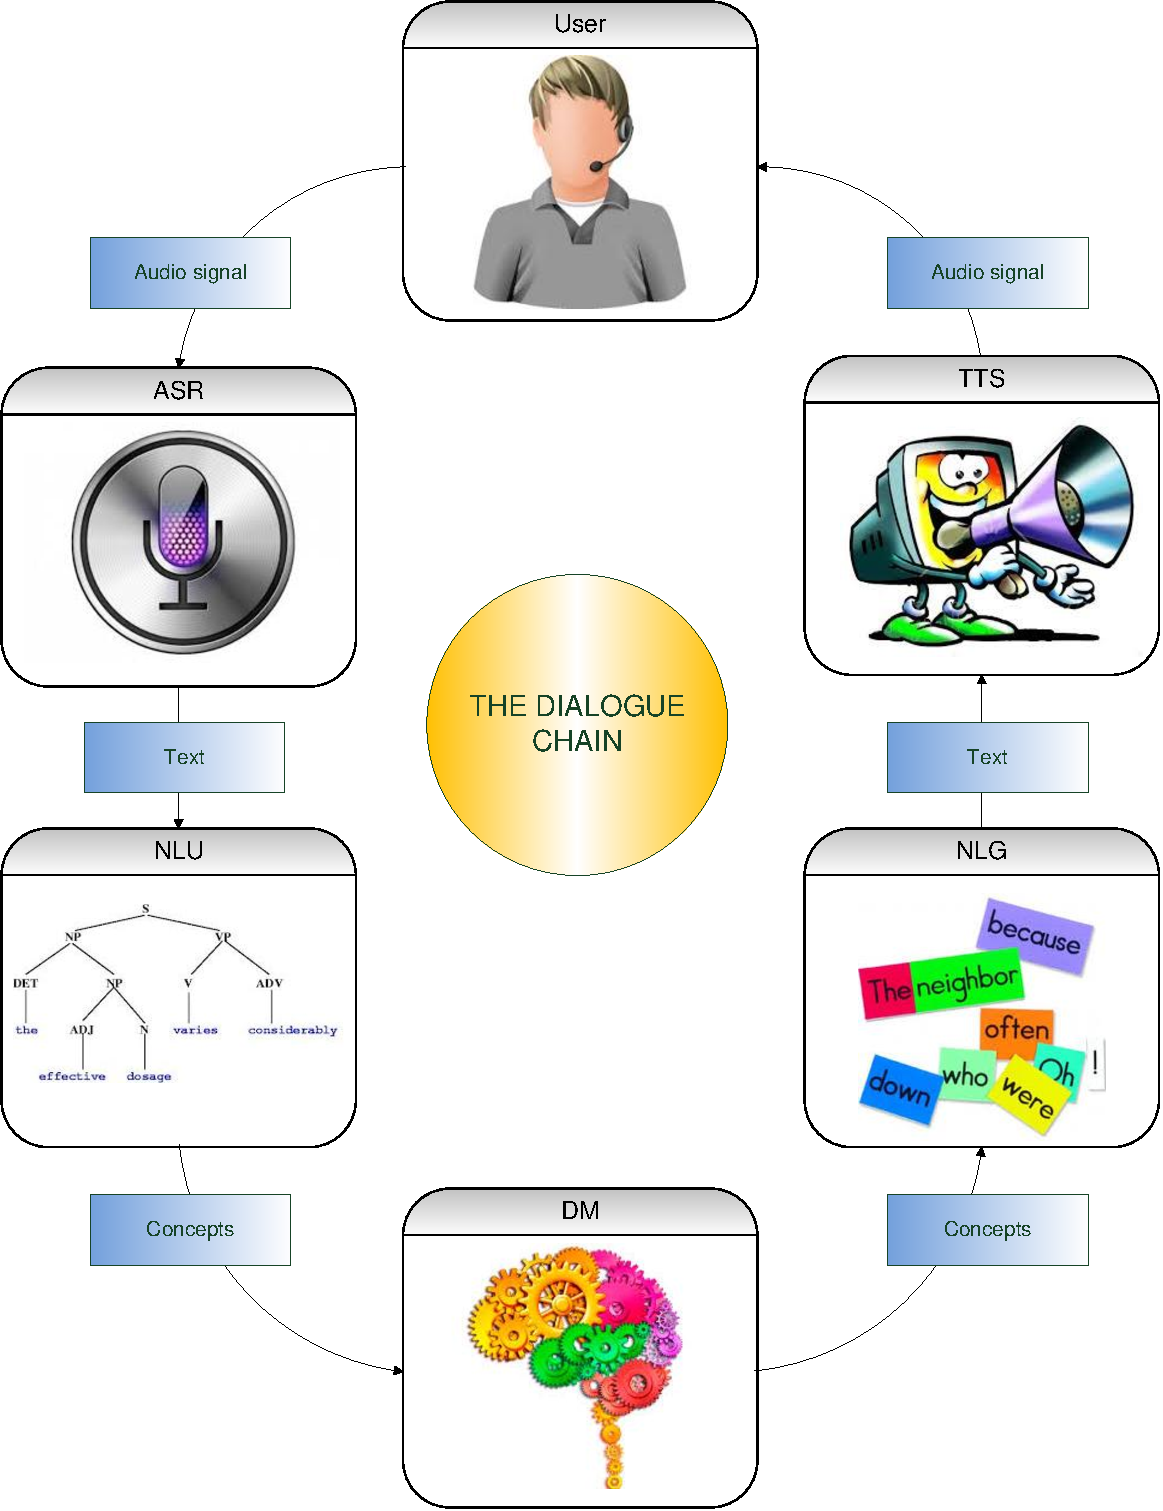
\includegraphics[scale=0.8]{figures/DialogueChain.pdf}
			\caption{The dialogue chain}
			\label{fig:dialchain}
		\end{figure}

		The classic architecture of an SDS is made of five main modules (Figure \ref{fig:dialchain}):
		\begin{enumerate}
			\item Automatic Speech Recognition (ASR): transforms the user's audio speech signal into text.
				\item Natural Language Understanding (NLU): outputs a conceptual representation of the user's utterance in text format.
				\item Dialogue Manager (DM): given the concepts extracted from the user's request, a response (in a conceptual format too) is computed.
				\item Natural Language Generation (NLG): transforms the concepts computed by the DM into text.
				\item Text-To-Speech (TTS): reads the text outputted by the NLG by using a synthetic voice.
		\end{enumerate}
		
		\subsubsection{Automatic Speech Recognition}

			%HK> Rajouter des références.
			Speech recognition technology is an old problem with long history. During the 1950s, a group of researchers from Bell Labs developed the first technology that is able to recognise digits from speech (in fact, speech perception has been under study since the early 1930s). Then, during the second half of the last century, new advances have made it possible to build ASR solutions with larger vocabulary and with no dependence on the user. In the 1960s, Hidden Markov Models (HMMs) were proved to be useful for speech recognition \cite{Gales2007} and they were the most popular technique two decades later. Commercial products using ASR technology had to wait until the 1990s to be finally released in the marked as they reached an interesting vocabulary scope (even though their accuracy and their delay were far behind the technology available today). Performances kept improving slowly and gradually until 2009, when Deep Learning algorithms were tested \cite{Mohamed2009,Deng2013} introducing huge improvement; the Word Error Rate (WER) decreased by 30\%. During the last six years, research continued in that direction giving birth to accurate and reactive speech recognition solutions (Google, Nuance, Sphinx, Kaldi...). These solutions also provide results incrementally in a continuous fashion. Therefore, ASR is less and less considered as a bottleneck in the development of spoken dialogue systems, and as it will be shown later, the delays they offer make it possible to design reactive incremental dialogue systems. Commercial off-the-shelf ASR solutions like Google ASR or Nuance products are able to recognise almost every word in many languages, including named entities. Finally, the ASR output is not only the text that the recognition algorithm figures out to be the best match for the input audio signal, but a list of the N most likely hypotheses and the corresponding confidence scores: it is called the N-Best. For instance, an 5-Best example is represented in Fig. \ref{fig:dialchain}.
			
			\begin{figure}
				\centering
				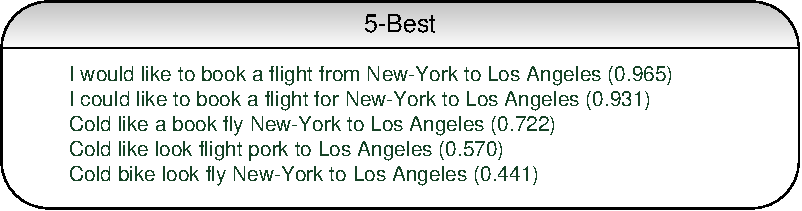
\includegraphics[scale=1]{figures/5BestEx.pdf}
				\caption{A 5-Best example corresponding to the sentence "I would like to book a flight from New-York to Los Angeles".}
				\label{fig:dialchain}
			\end{figure}
			
		\subsubsection{Natural Language Understanding}
		
			NLU is a sub-field of Natural Language Processing (NLP) whose scope is wider than the spoken dialogue field. Since the 1950s, researchers have been trying to develop several models and ontologies in order to automatically process natural language with several applications in sight: topic recognition, sentiment analysis, news filtering and analysis, natural speech processing...etc...The ambition manifested during 1950s and the early 1960s quickly had to face reality as the expected objectives were far from being reached. As a consequence, research in this area was significantly slowed down between the 1960s and the 1980s. During the last decade, NLP research has found a second wind thanks to new Machine Learning techniques, bringing them at the heart of lucrative businesses like recommendation and digital marketing. NLU refers to the set of techniques in order to make the machine understand the underlying structure of a text in natural language. To do so, a lexicon as well as an ontology (concepts and the links between them in a specific domain) should be built. Therefore, earlier NLU solutions are based on a set of handcrafted parsing rules, however, new statistical-based models \cite{Macherey2009} have been proven to be more robust and easy to generalise over domains. Also Deep Learning has also been applied to NLP showing interesting performances that NLU modules can benefit from \cite{Bengio2003,Collobert2011}.

		\subsubsection{Dialogue Management}
		
			As far as Dialogue Management is concerned, two decades ago, for the first time, dialogue has been modeled as Markov Decision Processes (MDPs) problem (see Sect. \ref{soa:rl}), hence being solved using reinforcement learning \cite{Levin1997a}. The dialogue state contains all the information needed to determine what is the best action to perform as well as the quality of that state (roughly speaking, to what extent it is desirable for the system to be at that state, in order to maintain the Markov property explained later). The possible actions in each state are the dialogue acts that the system can make while being at that state. In 2007, in order to represent the uncertainty over the user's intent (due to ASR or NLU imperfections), dialogues have been cast as Partially Observable Markov Decision Processes (POMDPs) \cite{Williams2007}. This gave raise to the notion of \textit{belief tracking} which objective is to keep a distribution over the possible user intents. Finally, existing dialogue systems are able to interact with the user in the domain they are built for only, however, during the last few years, researchers have been pushing the boundaries of domain  extension methods \cite{Gasic2013} and open-domain systems \cite{Pakucs2003,EkeinhorKomi2014,Wang2014}.
			
		\subsubsection{Natural Language Generation}
		
			The NLG task is the inverse of the NLU one: it translates dialogue acts' concepts into sentences. It started being used in the 1990s for purposes like financial news summary. A few start-ups and big companies also provide automatic text generation solutions that are used to quickly produce reports or official letters. The main challenge for such systems is to be able to generate a variety of different words, expressions and sentences in order for them not to be repetitive and for the result to be as realistic as possible. This is even more crucial when it comes to dialogue systems as they are supposed to simulate real conversations with the user, which is a highly variable. Nevertheless, in practice, template-based generation methods are the most widely used.
			
		\subsubsection{Speech Synthesis}

			During the 1930s, Bell Labs were not only interested in ASR but they also developed a new approach for the reciprocal task: the TTS (also known as \textit{speech synthesis}). The human speech is broken into small acoustic components that are sequentially pronounced by the system. They built the first machine demonstrating this mechanism: the Voder \cite{Dudley1939}. As far as this task is concerned, the challenge for the system is to sound as human-like as possible, in terms of phoneme transitions, speech rate and prosody. Two research threads tackle this problem in two different manners \cite{Tabet2011}: the first one uses corpus-based methods where the resulting audio is a combination of pre-recorded phonemes extracted from a corpus and the second one uses HMMs to generate a completely synthetic voice. Even though substantial advances have been accomplished since the Voder, it is still easy to distinguish between a synthesised and a real human voice.

	\subsection{Spoken dialogue systems evaluation}

		When building dialogue systems and improving them, it is necessary to determine metrics in order to measure their evolution. What makes a dialogue system better than another one? What metrics should be taken into account while evaluating dialogue systems? What are the most important characteristics of a dialogue system that should be improved?
		
		A distinction can be made between the evaluation of a dialogue system as a whole (\textit{usability} as it is called in \cite{Moller2007}) and the evaluation of the different components separately. In the second case, more standard metrics exist such as the Word Error Rate (WER) for the ASR or the CER (Concept Error Rate) when it comes to evaluating the NLU. Nevertheless, this is not the case for the DM: the usability evaluation is preferred to a local evaluation of the DM since they are very correlated \cite{Dybkjaer2004}. As a consequence, many evaluation frameworks for dialogue systems have been developed and used both in academia \cite{Walker1997,Hone2000,Schmitt2012} and industry \cite{Evanini2008,Witt2011}.

		In the PARADISE framework \cite{Walker1997}, a distinction is made between two kinds of metrics that are usually used for evaluating dialogue systems: objective and subjective metrics. The first category contains all the Key Performance Indicators (KPIs) that can be measured by an algorithm by accessing the dialogue logs only, whereas the second one is made of the user's appreciations of the dialogue quality or specific characteristics like human-likeness or to what extent the user enjoyed the dialogue experience.

		Objective metrics that are commonly used are the dialogues' mean duration and the task completion ratio. Generally speaking, these two metrics are correlated as the user gets impatient when the dialogue lasts for too long (the user can also get impatient for other reasons, like the repetition of the same system's dialogue act several times). Moreover, the user's speech rate and the way they communicate introduces some variability when using these metrics. Finally, it is legitimate to ask the question: are shorter dialogues the real desired objective? First, this depends on the type of dialogue system at hand. If it is designed for entertainment or companionship, then there is no need for seeking faster dialogue strategies. However, in the case of task-oriented dialogue, looking for shorter dialogues makes sense as a measure of efficiency. In these situations and especially for daily tasks, an efficiency threshold has to be necessarily reached in order for people to use the dialogue system at hand.

		Subjective metrics are generally gathered using a survey at the end of each dialogue or by making experts rate dialogues afterwards \cite{El-Asri2014b}. Several metrics can be collected this way: the global quality of the dialogue, naturalness/human-likeness, reactivity...etc...However, this also raises the problem of variability between users. Most often, they are asked to evaluate the system on a Likert scale (1 to 5 or 1 to 10), but a user answering 4 could be equivalent to another user answering 3 or 5. Therefore, the absolute evaluation is less significant than the relative one given a specific user.
	

\section{Incremental dialogue systems}
	
	\subsection{Principles}
	
		Currently deployed dialogue systems have a simple and rigid way of managing turn-taking. The interaction mode they offer is similar to a walkie-talkie conversation as the system waits for the user to finish her utterance before taking the floor and vice-versa (even though some systems allow the user to interrupt them). Such systems will be referred to as \textit{traditional dialogue systems} in this thesis.
    
		The first idea of incremental systems goes back to incremental compilers \cite{Lock1965}. An incremental compiler processes each new instruction independently from the previous ones. Therefore, a local modification of the code does not affect the whole result of the compilation. The idea of processing natural language in an incremental way is first introduced in \cite{Wiren1992} according to \cite{Kilger1995}. Instead of feeding modules with complete utterances, the input is pushed chunk by chunk (500ms of audio signal, one word of a sentence...etc...) making the output change several times before the end of the user's utterance. Nevertheless, in his book \textit{Speaking: From Intention to Articulation} \cite{Levelt1989}, Levelt analysed the mechanisms underlying the way humans formulate their ideas in natural language and already reported that the processes involved are incremental. The approach is closer to computational linguistics than psycholinguistics. The second part of the dialogue chain (DM, NLG and TTS) is analysed using a different terminology: the \textit{Conceptualizer}, the \textit{Formulator} and the \textit{Articulator}.

		As discussed in Sect. \ref{soa:inchuman}, in human to human conversation, the listener does not wait for the speaker to finish his sentence before processing it; it processes it as it is spoken. As a consequence, human beings perform a large panel of turn-taking behaviours while speaking, like backchanneling (\textit{aha}, \textit{yeah}...) or barging-in.
	
		To replicate these behaviours, a new generation of SDSs has been the focus of research for the last few years. An SDS is said to be incremental when it is able to process the user's speech on the fly. The input signal is divided into small chunks and the growing sentence is reprocessed at each new chunk \cite{Schlangen2011}. Table \ref{tab:incrnluex} gives an example illustrating the functioning of an incremental NLU module (in a hotel room booking service). For the sake of simplicity, processing delays are neglected.
	
		\begin{table}[th]
			\vspace{2mm}
			\centerline{
				\begin{tabular}{|l|l|l|}
					\hline
					\textbf{Time step} & \textbf{NLU input} & \textbf{NLU output} \\
					\hline
					1 & I & empty \\
					\hline
					2 & I won't & empty \\
					\hline
					3 & I would & empty \\
					\hline
					4 & I would like to & empty \\
					\hline
					5 & I would like to cook a & empty \\
					\hline
					6 & I would like to book a room & \textbf{action:} BOOK \\
					\hline
					7 & I would like to book a room on May & \textbf{action:} BOOK \\
					\hline
					8 & I would like to book a room on May 7$^{th}$ & \textbf{action:} BOOK \\
					& & \textbf{date:} 05-07 \\
					\hline
					9 & I would like to book a room on May 17$^{th}$ & \textbf{action:} BOOK \\
					& & \textbf{date:} 05-17 \\
					\hline
					10 & I would like to book a room on May 17$^{th}$ and I will & \textbf{action:} BOOK \\
					& & \textbf{date:} 05-17 \\
					\hline
					11 & I would like to book a room on May 17$^{th}$ and I will & \textbf{action:} BOOK \\
					& be driving & \textbf{date:} 05-17 \\
					& & \textbf{parking:} YES \\
					\hline
				\end{tabular}
			}
			\caption{Example of incremental NLU processing}
			\label{tab:incrnluex}
		\end{table}

	\subsection{Advantages of incremental processing}

                Before discussing the different reasons why incremental processing should be preferred to rigid turn-taking, it is important to note that a few studies with real users have shown that incremental dialogue systems offer a better user experience. For instance, in \cite{Aist2007}, an ordinal regression has been performed between the user satisfaction and several features with a flag for incremental processing among them. A significant correlation between incremental processing and the global user satisfaction has been found. Other studies also confirm the advantage of incremental speech processing \cite{Skantze2009,El-Asri2014a,Zhao2015}.

                As discussed in Section \ref{soa:humanlike}, human-likeness is a legitimate goal for dialogue systems (at least worth trying). When talking to each other, humans perform a rich set of turn-taking phenomena (see Section \ref{soa:ttphuman}) and in spite of the fact that they do not talk in a rigid walkie-talkie manner, they manage to avoid desynchronisations and to keep a conversation that is going forward. Replicating these behaviours from the machine's point of view can therefore be interesting. It might be expected that the user feels more at ease while using a more human turn-taking mode hence pushing the human metaphor even further.

                The other aspect that is interesting about incremental dialogue is reactivity. As the system processes the user's request before its ends, it is possible to design accurate end-point detection in order to detect the end of this request as soon as possible \cite{Raux2008}. Moreover, incremental dialogue systems can interrupt the user to report a problem, like in the following example:
								
								\begin{dialogue}
									\speak{USER}{I would like to book a room for tomorrow with ...}
									\speak{SYSTEM}{Sorry, we are full tomorrow.}
								\end{dialogue}
								
								This can help the user get to her goal faster but one should be very careful about the way it is implemented as there is a risk that user interruption actually harms the user experience (even though the intent is to go faster, see Section \ref{soa:challengesincr}). Nevertheless, a corpus study led in \cite{Ghigi2014} showed that when users are interrupted, they tend to adopt a more sober way of expression, hence directly increasing the dialogue efficiency but also indirectly as the risk of misleading off-domain words and expressions is reduced \cite{Zhao2015}.
								
								Early barge-in both from the user and the system's side is also a way to limit desynchronisations. An example of a desynchronised dialogue could be (inspired by the NUMBERS domain described in \cite{Skantze2009}):
								
								\begin{dialogue}
									\speak{USER}{01 45 38 37 89}
									\speak{SYSTEM}{01 45 28 37 89}
									\speak{USER}{No, not 28 but 38}
									\speak{SYSTEM}{Sorry, you mean 28 38}
									\speak{USER}{What?}
									\speak{SYSTEM}{28 38 1} \textit{(The system understood "One" instead of "What?")}
								\end{dialogue}
								
								In this example, the user could have reported the mistake earlier if he could barge-in:
								
								\begin{dialogue}
									\speak{USER}{01 45 38 37 89}
									\speak{SYSTEM}{01 45 28...}
									\speak{USER}{No, 38}
									\speak{SYSTEM}{Ok. 01 45 38}
									\speak{USER}{31 89}
									\speak{SYSTEM}{31 89}
								\end{dialogue}
								
		Another interesting aspect about incremental dialogue systems is that they can leverage multimodality \cite{Fink1998}. In fact, there are two aspects of multimodality and they can both benefit from incremental processing:
								
		\begin{itemize}
		   \item \textbf{Input multimodality:} Most researchers in the community refer to this aspect when talking about mutimodal systems. A system input can be multimodal in the sense that it can handle speech input, but also text, gesture or eye-gaze for example. The main challenge faced by this kind of setup is the problem of mixing these inputs in order to infer the correct user intent. In the case of multimodal systems, the world is considered as a flow of information coming from multiple sources of information \cite{Chao2012,Rosenthal2013}. The different modalities are not necessarily sampled with the same rate nor support the same delays, therefore, it is important to find convenient ways to synchronise them.
		   \item \textbf{Output multimodality:} The machine can also use different channels of information while communicating \cite{Matthias2009}. For example, the speech modality can be used at the same time as a moving avatar with facial expressions (the Furhat for example \cite{Skantze2015}). It can also be coupled with the input multimodality paradigm to create highly interactive interfaces like \cite{Johnston2014}.
		\end{itemize}
		

	\subsection{New challenges raised by incremental dialogue processing}
	\label{soa:challengesincr}
    
		%HK> Citer Dan Povey pour Kaldi.
		The first problem to consider when talking about incremental spoken dialogue systems is the question of ASR \textit{latency}, which is the time needed by the recognition algorithm to provide the text output corresponding to an audio signal. As discussed earlier, the ASR accuracy has been a bottleneck in the development of spoken dialogue systems for many years but thanks to recent advances in this field, it is no longer the case. Similarly, incremental dialogue systems require quick responses from the ASR but speech recognition modules have been too slow for many years which was a limiting factor in the development of incremental dialogue processing. But, in the last few years, ASR technology has become reactive enough \cite{Breslin2013,Platek2014}. Still, it is important to be aware that there is a tradeoff between the accuracy, the vocabulary size and the latency. Kaldi, which is an ASR solution designed by researchers (and which is mostly used by them), makes it possible to design one's own acoustic and language model as well as setting one's own parameters in order to control this tradeoff. Off-the-shelf solutions like Google ASR do not give the user such possibilities (however, accuracy and delays in open domain are well balanced for most applications).

		%HK> Citer Ethan et Jason au sujet de l'instabilité si ce n'est déjà fait.
		If the successive partial results of an incremental ASR module are observed during a user's utterance, it is likely that the progression they follow is not monotonous. In other words, a partial result is not guaranteed to be a prefix of results to come. The following example showing successive ASR results illustrates this phenomenon:

		\begin{enumerate}
			\item Euh
			\item I
			\item Euh good
			\item iPod
			\item I would
			\item I good bike
			\item I would like
		\end{enumerate}

		This phenomenon is called ASR \textit{instability} (or stability depending on the sources) \cite{Selfridge2011}. This factor is also related to the tradeoff between latency and accuracy as preferring fast ASR over accurate ones can lead to very unstable results (the system is not given enough time to compute accurate results most of the time, thus ending up delivering wrong partial results frequently), and vice-versa.
		
This leads to one of the main challenges raised by incremental processing: the ability to \textit{revise} the current hypothesis. All the modules in the dialogue chain are impacted by this problem. As an illustration, suppose that the user interacts with an incremental personal assistant on her phone and makes the following request \textit{Please call the number 01 45 80 12 35}. The last digit is first understood as being 30 and then 35, therefore, if the system is too reactive, there is a risk that it starts calling the wrong number and maybe start uttering the sentence \textit{Ok, calling 01 45 80 12 30}. Afterwards, the system understands 35 instead of 30 hence needing a correction mechanism in order to stop the TTS, to cancel the call, to perform a new one and to provide a new answer to the user. Nevertheless, even though the system at hand is equipped with such a mechanism, using it very often is not an optimal way of managing incremental input as it causes extra delay as well as non-natural behaviour (stopping the TTS and starting again with another utterance). This introduces a similar tradeoff to the one discussed for the ASR module but from the DM perspective: if decisions are taken too quickly, it is likely that some of them are wrong hence activating the correction mechanism. On the other hand, if the DM is slow to take action, then it lacks reactivity and there is no point for it to be incremental. As a consequence, it is important to determine the right moment to commit to the current partial utterance and to take action based on it \cite{Raux2008,Lu2011}.

		Incremental NLG also raises new problems which are illustrated in \cite{Baumann2013}. In this paper, a system has to describe a car's trajectory in a virtual world. When the latter approaches an intersection where it has to turn right or left (no road straight ahead), then the system utters something like \textit{The car drives along Main Street and then turns...euh...and then turns right}. In this example, the system is sure that the car is going to turn which makes it possible for it to commit to the first part of the sentence with no risk. However, this is not always the case as a new chunk of information from the user can change the whole system's response. In this thesis, the NLG is not incremental as the DM's response is considered to be computed instantly at each new micro-turn (event though it is not necessarily stable and it can vary from micro-turn to micro-turn). Finally, in purely vocal applications, computing the NLG results incrementally does not make much sense as the user's and the system's utterances do not overlap most of the time \cite{Sacks1974}. However, this is an interesting behaviour as far as multimodal applications are concerned.

		Building an incremental TTS module can also be very tricky. In order for the synthetic voice to be the most human-like as possible, prosody should be computed accurately and to do so, the sentence's structure and punctuation have to be taken into account. This information is no longer given in the case of incremental TTS or it arrives too late. \cite{Baumann2014} proposes a method for coping with the problem. 


	\subsection{Existing architectures}
		\subsubsection{Sequential paradigm}
			
			A general abstract model of incremental dialogue systems has been introduced in \cite{Schlangen2011}. In this approach, the dialogue chain is maintained and each one of the five components is transformed into its incremental version. This view of incremental dialogue systems will be referred to as the \textit{sequential paradigm}.
				
			Each module is composed of three parts, the Left Buffer (LB), the Internal State (IS) and the Right Buffer (RB). As described in Section \ref{soa:architecture}, each module is also characterised by the type of input it processes as well as the type of output it computes. In incremental dialogue, all these data flows have to be divided into small chunks which are called Incremental Units (IU). For example, the audio signal that is given as an input to the ASR module can be divided into 500ms chunks that are processed one by one. Each IU is first added to the LB, then it is taken by the IS for processing and once a result is available, a new IU of a new kind is outputted in the RB. The RB of one module is the LB of the following one in the dialogue chain so the data propagation through the dialogue system is insured.
			
			Because of the ASR instability, new IU in the LB does not necessarily imply that a new IU will be pushed into the RB on top of the ones that already existed there. An example given in \cite{Schlangen2011} is the following: suppose the user utters the number \textit{forty} which processed incrementally, then first the ASR outputs \textit{four} and then \textit{forty}. As a consequence, the second hypothesis does not complete the first one but it replaces it in the RB. This phenomenon will be discussed in more details in Chapter \ref{ch:simulation}.
			
			Adopting this paradigm is a natural way of enhancing traditional dialogue systems with incremental capabilities. It is interesting from a computational and design point of view as the different tasks are separated. Therefore, one is able to evaluate the different components independently \cite{Baumann2011} and have a global view to determine which area still needs improvement.

		\subsubsection{Multi-layer paradigm}
		
			The problem of dialogue management in traditional dialogue systems can be formulated as follows: at each dialogue turn, given the dialogue context (including the last user's utterance), what is the right dialogue act to perform? In the incremental frame, this definition no longer holds as dialogue acts are no longer attached to dialogue turns. Therefore, one way to tackle the problem is to split the dialogue management task in two components, the high-level and the low-level handlers. This paradigm is directly motivated by Austin's, Searl's and Clark's contributions discussed in Section \ref{soa:dialogueacts} as the high-level module handles illocutionary acts (the communicative track) whereas the low-level one manages phonetic acts (the meta-communicative track).
				
				As reported in \cite{Lemon2003}, this approach is more in alignment with results in the psycholinguistic field. The phenomena observed at the phonetic level are complex, and the interaction happen on multiple levels, not always following the classical dialogue chain. Having a separate module for handling these phenomena is therefore a more natural paradigm.
				
				Switching from the traditional dialogue management approach to the incremental one is also a transition from discrete time to continuous time, from a synchronous to an asynchronous processing \cite{Raux2007}. The low-level module is continuously (approximated by a high frequency processing in computers) listening to the outside world and waiting for events that might be interesting to communicate to the high-level handler. In that case, the latter returns actions (dialogue acts) and it is the role of the low-level module to choose whether to retrieve them to the user or not as well as choosing the right moment in case it decides to speak.
				
				Finally, starting from a traditional dialogue system, it is easier and more straightforward to transform it into an incremental one if one adopts this paradigm. Adding an extra low-level module to the dialogue manager is enough \cite{Selfridge2012a}. At each new incremental input, this module sends the whole partial utterance from the beginning of the current turn to the dialogue manager and gets a response. Based on that and eventually some other features, it decides whether to take the floor or not. As most of the requests sent to the dialogue manager are "fake" as they are not meant to be acted on, they should not affect the dialogue context. Therefore, either multiple instances of the dialogue manager are used, either the dialogue context is saved and restored at each new request, unless the low-level module decides to take the floor (see Chapter \ref{ch:architecture} for additional explanations).

\section{Reinforcement Learning}
\label{soa:rl}

	\subsection{Reinforcement in biology}
    
		Reinforcement Learning (RL) is a sub-field of machine learning where an agent is put into an environment to interact with, and figures out through the process of \textit{trial and error} what the best actions to take are, given a reward function to maximise \cite{Sutton1998} (see Figure \ref{fig:rlscheme}).
			
			\begin{figure*}[ht]
				\centering
				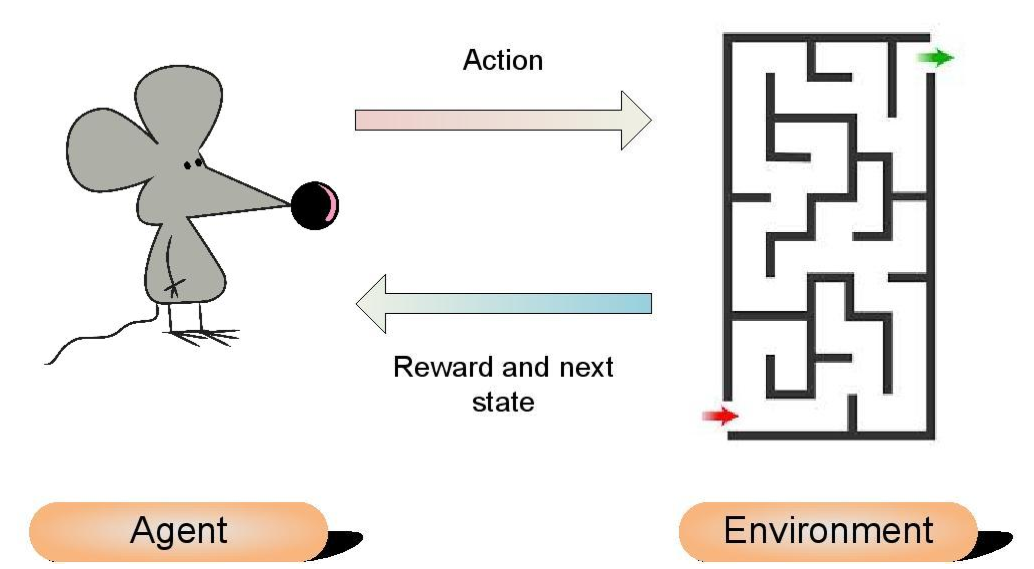
\includegraphics[scale=0.8]{figures/AgentEnv.pdf}
				\caption{The interaction cycle between the agent and the environment in reinforcement learning}
				\label{fig:rlscheme}
			\end{figure*}
			
			It was first inspired by the field of biology where living organisms are considered as the agents. Rewards are associated with stimuli that the agent seeks like food for example. Conversely, punishments are stimuli that it tries to avoid like important heat for instance. In \cite{Thorndike1898}, hungry animals where put in enclosures where the only way to escape and find food is to perform some simple act (pulling at a loop of cord, pressing a lever, stepping on a platform...). If after a certain period of time they were not able to escape, they are taken out of the box without being immediately fed. This experiment showed how animals were able to learn what to do in order to escape from the enclosure.
			
			During the last two decades, similarities between reinforcement learning and neurons behaviours in the brain were also discovered. In \cite{Schultz1995,Schultz1998}, similarly to the previous experiment, monkeys were put in situations where the accomplishment of an action is necessary to get food. Then the reaction of their dopamine neurons was analysed. Among many other applications where reinforcement learning meets neuroscience, \cite{Doya2007} commented on this experiment: \textit{Although dopamine neurons initially responded to the rewards, when those rewards became fully predictable from preceding sensory cues, such as light and sound, their reward responses went away. Instead, dopamine neurons started to respond to reward-predictive sensory cues. If the reward is omitted after learning, dopamine neuron firing was suppressed at the timing when reward delivery is expected. These are interesting findings on their own, but most exciting for those who are familiar with reinforcement learning theory because it exactly matches what the TD error does}.
			
		\subsection{Markov Decision Processes}
        
			The most common model consists in casting the agent as a Markov Decision Process (MDP) which is a quintuple $\mathcal{M} = (\mathcal{S},\mathcal{A},\mathscr{T},\mathscr{R},\gamma)$ where:
			\begin{itemize}
					\item $\mathcal{S}$ is the \textit{state space}. At each time step $t$, the agent is in some state $s_t \in \mathcal{S}$.
					\item $\mathcal{A}$ is the \textit{action space}. At each time step $t$, the agent decides to take action $a_t \in \mathcal{A}$.
					\item $\mathscr{T}$ is the \textit{transition model} where each $(s,a,s')$ in $\mathcal{S} \text{x} \mathcal{A} \text{x} \mathcal{S}$ is associated with a real number in $[0,1]$ corresponding to the probability $\mathbb{P} (s_{t+1} = s'|s_t = s, a_t=a)$. A more compact notation will be used in the following: $\mathscr{T}_{ss'}^a = \mathscr{T} (s,a,s')$.
					\item $\mathscr{R}$ is the \textit{reward model}. Let $r$ be the immediate reward due to taking action $a$ in state $s$, then $\mathscr{R}$ is the set of distributions of $r$ for every $(s,a) \in \mathcal{S} \text{x} \mathcal{A}$. The following notation will be used in the rest of this chapter: $\mathscr{R}_{ss'}^a = \mathbb{E} [\mathscr{R} (s,a,s')|s,a,s']$.
					\item $\gamma \in [0,1[$ is referred to as the \textit{discount factor}. In the RL framework, the aim of the agent is not to maximise the immediate reward but the \textit{expected return}, where the return $R_t$ is defined as follows:
					
					\begin{eqnarray}
						R_t & = & r_{t+1} + \gamma r_{t+2} + \gamma^2 r_{t+3} + ... \nonumber \\
						& = & \sum_{k=0}^\infty \gamma^k r_{t+k+1} \label{eq:return}
					\end{eqnarray}
					
					Therefore, when $\gamma = 0$, the agent maximises the immediate reward only and when $\gamma$ tends towards 1, the agent maximises the sum of all the future rewards. In other words, the parameter $\gamma$ controls how far-sighted is the agent in terms of future rewards.
	\end{itemize}
			
			A \textit{policy} $\pi : \mathcal{S} \rightarrow \mathcal{A}$ is a mapping between the state space and the action space. An agent is said to follow the policy $\pi$ when for each time $t$, it takes the action $a_t = \pi(s_t)$. A policy can also be stochastic, in which case, $\pi (s,a)$ denotes the probability of choosing action a when the agent is at state s. A key aspect of MDPs is the \textit{Markov property}. Being at state $s$ is the only information available to predict the future, and adding information about what happened during previous time steps has no power of prediction. Therefore, given a policy, each state $s \in \mathcal{S}$ is associated with a value $V^\pi (s)$ which is the expected return when at this state and following the policy $\pi$ afterwards:
				
				\begin{eqnarray}
					V^{\pi} (s_t) & = & \mathbb{E} [R_t | s_t, \pi] \label{eq:valuefunc}
				\end{eqnarray}
					
			Another interesting quantity is the expected return knowing the current state but also the next action, after which $\pi$ is followed. This is referred to as the Q-function:
				
				\begin{eqnarray}
					Q^{\pi} (s_t,a_t) & = & \mathbb{E} [R_t | s_t, a_t, \pi] \label{eq:qfunc}
				\end{eqnarray}
					
			Given the definition of $R_t$, one can notice that 
			\begin{eqnarray}
					V^{\pi} (s_t)   & = & \mathbb{E} [R_t | s_t, \pi] \nonumber \\
					& = & \mathbb{E} [r_t + \gamma \sum_{k=0}^\infty \gamma^k r_{(t+1)+k+1} | s_t, \pi] \nonumber \\
					& = & \mathbb{E} [r_t + \gamma R_{t+1} | s_t, \pi] \nonumber \\
					& = & \mathbb{E} [r_t + \gamma \mathbb{E} [R_{t+1}|s_{t+1}, \pi] | s_t, \pi] \nonumber \\
					& = & \mathbb{E} [r_t + \gamma V^{\pi} (s_{t+1}) | s_t, \pi] \label{eq:vbellman}
			\end{eqnarray}
					
		This is known as the Bellman equation for $V^{\pi}$ and it can also be written for the Q-function, as follows
				
				\begin{eqnarray}
					Q^{\pi} (s_t,a_t) & = & \mathbb{E} [r_t + \gamma Q^{\pi} (s_{t+1}, \pi(s_{t+1})) | s_t, a_t, \pi] \label{eq:qbellman}
				\end{eqnarray}
	
	\subsection{Reinforcement Learning}
            
			A natural question that can be asked at this point is: how are these values computed? In reinforcement learning, this is known as the \textit{evaluation problem}. The transition model $\mathscr{T}$ and the reward model $\mathscr{R}$ are the elements that define the dynamics of the MDP. If they are known, $V^{\pi}$ can be directly computed:
			
			\begin{eqnarray}
					V^{\pi} (s)   & = & \mathbb{E} [R_t | s_t = s, \pi] \nonumber \\
					& = & \sum_{a \in \mathcal{A}} \pi (s,a) \mathbb{E} [R_t | s_t = s, a_t = a, \pi] \nonumber \\
					& = & \sum_{a \in \mathcal{A}} \pi (s,a) \mathbb{E} [r_t + \gamma R_{t+1} | s_t = s, a_t = a, \pi] \nonumber \\
					& = & \sum_{a \in \mathcal{A}} \pi (s,a)  \sum_{s' \in \mathcal{S}} \mathscr{T}_{ss'}^a (\mathscr{R}_{ss'}^a + \gamma \mathbb{E} [R_{t+1} | s_{t+1} = s', \pi]) \nonumber \\
					& = & \sum_{a \in \mathcal{A}} \pi (s,a)  \sum_{s' \in \mathcal{S}} \mathscr{T}_{ss'}^a (\mathscr{R}_{ss'}^a + \gamma V^{\pi} (s')) \label{eq:dynprog}
			\end{eqnarray}
					
			It is possible to define an order over the policies. Saying that $\pi_1$ is better that $\pi_2$ means that for all the states $s$, $V^{\pi_1} (s) \geq V^{\pi_2} (s)$. It can be shown that there exists at least one policy that is better than all the others: it is called the \textit{optimal policy} ($\pi^*$). To simplify the notations, $V^{\pi^*}$ will be referred to as $V^*$ and it is defined as
				
				\begin{eqnarray}
					\forall s \in \mathcal{S}, \text{ } V^* (s) & = & \max_\pi V^\pi (s) \label{eq:voptim}
				\end{eqnarray}
					
			Similarly, one can define $Q^*$ as
				
				\begin{eqnarray}
					\forall (s,a) \in \mathcal{S} \text{x} \mathcal{A}, \text{ } Q^*(s,a) & = & \max_\pi Q^{\pi}(s,a) \label{eq:qoptim}
				\end{eqnarray}

			The aim of reinforcement learning is to learn the optimal policy. Similarly to what has been shown for $V^{\pi}$, if the transition and the reward models are known, the Bellman equation corresponding to $V^*$ (called the \textit{Bellman optimality equation}) can be written with respect to these models (similarly to \ref{eq:dynprog}):
							
				\begin{eqnarray}
					V^*(s) & = & \max_a \sum_{s' \in \mathcal{S}} \mathscr{T}_{ss'}^a (\mathscr{R}_{ss'}^a + \gamma V^*(s')) \label{eq:vbellmanoptim}
				\end{eqnarray}
			
			A similar form can be also be shown about the Q-function
							
				\begin{eqnarray}
					Q^*(s,a) & = & \sum_{s' \in \mathcal{S}} \mathscr{T}_{ss'}^a (\mathscr{R}_{ss'}^a + \gamma \max_{a' \in \mathcal{A}} Q^*(s',a')) \label{eq:qbellmanoptim}
				\end{eqnarray}

			A set of \textit{Dynamic Programming} methods exist in order to efficiently solve these kinds of equations and come up with the optimal policy given the transition and the reward model (knowing $Q^*$ implies knowing $\pi^*$ as the latter is the greedy policy with respect to the former Q-function, in the sense that $\pi^*(s) = \argmax_a Q^*(s,a)$). However, even though this kind of approaches are theoretically interesting, they only have a few practical applications as most of the times, $\mathscr{T}$ and $\mathscr{R}$ are unknown. The agent learns directly from interacting with the environment (\textit{model-free} approach).
			
			It is possible to try to learn $\mathscr{T}$ and $\mathscr{R}$ first and then applying a \textit{model-based} algorithm to figure out the optimal policy. Nevertheless, this is not necessary as most algorithms compute the optimal policy by directly estimating the Q-function. This can be done in a straightforward fashion by running several episodes\footnote{To keep things simple in this introduction to reinforcement learning, the MDP is considered to eventually stop.}, computing the returns for each state-action couple and for each episode, then using the mean return over all the episodes as an estimate of $V^\pi$ or $Q^\pi$. Algorithms using this kind of approach belong to the category of \textit{Monte-Carlo methods}.
			
			However, as the agent interacts with the environment, it encounters a similar dilemma to the one faced in the bandit problem \cite{Berry1985,Bubeck2012}: how to manage the trade-off between \textit{exploration} and \textit{exploitation}. While being at a state $s \in \mathcal{S}$, the agent can choose one action among many. Let us say that the Q-function is initialised as a zero function. Therefore, at the beginning the agent has no preference and selects a random action. If this yields a positive reward, then the agent has the choice between these two options to make the next decision:
			
			\begin{enumerate}
				\item Making the same decision again as it already knows that it is likely to generate a positive reward.
				\item Picking another action because it may yield an even greater reward.
			\end{enumerate}
			
			In the first case, the agent is exploiting its current knowledge of the environment whereas in the second case, it is said to be exploring as it is increasing its knowledge about the environment (with the risk of generating low or negative rewards in the meanwhile). Because rewards are stochastic, it is not obvious to determine whether sufficient data is available to trust our estimates and start exploiting most of the time. This is a difficult problem and a simple way to deal with it is to use the $\epsilon$-greedy approach, where the agent chooses a random action with a probability of $\epsilon$ and sticks to the greedy action (with respect to the current estimated Q-function) the rest of the time. Nevertheless, more robust solutions have already been suggested like Upper Confidence Bound (UCB) \cite{Auer2002} for the bandit problem and Upper Confidence Reinforcement Learning (UCRL) \cite{Auer2005} for reinforcement learning.
			
			Reinforcement learning algorithms keep evaluating the current policy and at the same time, altering that policy in order to improve it. A naive approach would be to fix the current policy and to perform as many evaluation iterations as necessary in order to gain a certain confidence over the estimations of $V$ or $Q$ and then to derive a new policy to follow, given these values. This is known as \textit{Policy Iteration} but this is not the most efficient way to proceed (so many iterations are needed). In fact, performing only one evaluation iteration before the next policy improvement step can be shown to be enough, keeping the convergence guarantees. This is referred to as \textit{Value Iteration}. Also, the notion of iteration can be viewed differently given the approach and the algorithm at hand. In order to refer to the general idea of intertwining evaluation and control, the expression \textit{General Policy Iteration} (GPI) is used.
			
			In fact, it is also possible to evaluate $V$ or $Q$ in an even more fine-grained manner. Instead, of waiting until the end of the episode to update these values, it is possible to do it after each new decision. That is what \textit{Temporal-difference (TD) methods} do. In comparison with the Monte-Carlo approach, the new sample for $V^\pi(s)$ or $Q^\pi(s,a)$ is no longer the real return obtained in the episode but an estimated one using the Bellman equation. In the case of the \textit{sarsa} algorithm\footnote{See \cite{Sutton1998} for the algorithm description.}, the Q-function is updated as follows\footnote{At this point, $V$ will no longer be used, as $Q$ is the most commonly used in reality. $V$ is mostly used for pedagogical purposes.} ($\alpha_t$ being a decreasing parameter with time):
			
			\begin{eqnarray}
				Q_t(s_t,a_t) & = & Q_t(s_t,a_t) + \alpha_t [r_t + \gamma Q_t(s_{t+1},\pi_t(s_{t+1})) - Q_t(s_t,a_t)] \label{eq:sarsaupdate}
			\end{eqnarray}
			
			It is important to notice that $a_{t+1}$ is the action chosen by following the current estimated policy derived from Q ($\epsilon$-greedy for example) and which will be actually followed in the next step. The sarsa algorithm is therefore called an \textit{on-policy} algorithm. These conditions can be relaxed giving birth to another category of algorithms, the \textit{off-policy} ones. The most famous is \textit{Q-Learning}\footnote{See \cite{Sutton1998} for the algorithm description.} \cite{Watkins1989} where the Q-function is updated as follows:
			
			\begin{eqnarray}
				Q_t(s_t,a_t) & = & Q_t(s_t,a_t) + \alpha_t [r_t + \gamma \max_a Q_t(s_{t+1},a) - Q_t(s_t,a_t)] \label{eq:qlearningupdate}
			\end{eqnarray}
			
			Here, the policy used for evaluation is not necessarily the one that is followed.

\section{Reinforcement learning in spoken dialogue systems}
	
	\subsection{In the litterature}
	
		Reinforcement learning has been first applied to dialogue systems in \cite{Levin1997b} and since then, it has been the leading machine learning framework in the field. The dialogue state at time $t$ is generally determined by the history of dialogue acts since the beginning of the dialogue. At each turn, the set of actions is made of all the possible answers at that time.
		
		Dialogue has first been cast as an MDP. For instance, one of the earliest applications of this framework is described in \cite{Singh1999}. The system involved handles a simple slot-filling task where it decides whether to ask for all the slots at once, to ask for a specific slot or whether to perform a confirmation. In order to handle ASR imperfections, Partially Observable Markov Decision Processes (POMDPs) \cite{Young2006,Williams2007} can be used. In this framework, the dialogue state is replaced by a distribution over all possible states which is a more natural way of modeling uncertainty, however, they are more complex and more difficult to scale \cite{Lemon2007}. Another interesting approach that has been applied to dialogue systems is Hierarchical Reinforcement Learning \cite{Cuayahuitl2007}. It is meant to handle large state spaces with an important dimensionality, which is often the case in dialogue management. It requires the dialogue to be cast as a Semi-Markov Decision Process (SMDP) \cite{Bradtke1994,Barto2003}. Huge and complex state spaces are also dealt with by using \textit{summary states} in most cases, which can be built in several ways. Nevertheless, new approaches using Deep Reinforcement Learning methods started being developed very recently \cite{Cuayahuitl2015}; instead of using handcrafted features for state representation, raw data is directly fed to a deep neural network.
		
		Also, it is noteworthy that even though the main focus in this thesis is dialogue management, reinforcement learning has also been applied to the NLG task in order to optimise information presentation \cite{Walker2000,Rieser2011b} and even TTS to decide what kind of prosody should be used \cite{Bretier2010}.
	
	\subsection{Spoken dialogue systems at Orange and the LIA}

        	        Important research work have been accomplished at Orange during the CLASSIC project. It was mainly focused on the problem of reconciling academic research with industrial activity \cite{Paek2007}. A new reinforcement model has been developed (in the continuity of work done by \cite{Singh2002,Williams2008}): the Module Variable Decision Process (MVDP) \cite{Laroche2010a}. It has been implemented in an appointment scheduling task hence giving birth to the first dialogue system learning on-line (directly from experience) \cite{Putois2010}. In addition, other research efforts have been made in order to make reinforcement results accessible directly in design mode.

                During the course of this thesis, Orange has also focused on other aspects of dialogue such as reinforcement learning convergence speed \cite{El-Asri2013a}, interaction quality prediction \cite{El-Asri2012,El-Asri2014d} as a well as reward function inference and state space representation. In \cite{El-Asri2012}, reward shaping is used to learn a reward function directly from a corpus of dialogues with experts' ratings. Moreover, a new framework called Genetic Sparse Distributed Memory for Reinforcement Learning (GSDMRL) has been proposed \cite{El-Asri2016} which purpose is to compute a state representation that is adapted to the utility function to maximise.
								
								Vocal assistants are becoming a part of our everyday life since their introduction in the market. They are able to perform several tasks but they are still static and limited. Therefore, Orange also investigates solutions to make dialogue systems able to manage several tasks by merging dialogue models of different applications which also makes it easily extensible \cite{EkeinhorKomi2014}. Finally, designing systems that can listen to human/human conversations and make decisions based on them is also a topic that is tackled in this lab \cite{Barlier2015}. It is motivated by several applications like connected houses, meeting rooms, call centers...

                As far as the LIA (Laboratoire Informatique d'Avignon) is concerned, several subjects concerning human-robot interaction (mainly through dialogue) and Natural Language Processing (NLP) are are driving the research activity. Among them:

                \begin{itemize}
                  \item \textbf{Interactive Voice Response (IVR):} The objective of the Port-MEDIA project is to design robust multi-language and multi-domain models for IVR, an IVR being the interface between a user and a database.
                  \item \textbf{Human-Robot interaction:} The main objective of this research field is to design adaptive algorithms to improve the interaction between humans and robots. These are mainly reinforcement learning algorithms. The robot performs poorly at an early stage but with experience, through an error-trial process, it learns to better itself and improve the interaction quality.
                  \item \textbf{Automatic Speech Translation:} French/English and English/French translation algorithms have been built in collaboration with the LIG (Laboratoire Informatique de Grenoble), based on the Mooses Toolkit. In 2001, the French/English algorithm won second place in the international campaign WMT.
                \end{itemize}

	
	\subsection{Dialogue simulation}
	
		A couple of decades ago, with the development of the dialogue systems research field, the need for evaluation means in order to assess their quality started getting more and more important. Therefore, researchers turn to user simulation methods (also referred to as user modeling). In \cite{Eckert1997}, some of the advantages of these techniques are depicted: the possibility to quickly generate corpora for machine learning techniques at a low cost, easy modeling of different user populations and the possibility of using the same user model across different concurrent dialogue systems for comparison. Nevertheless, the authors recognise that user simulation cannot totally replace interactions with real users in the process of designing reliable dialogue systems: \textit{we believe that tests with human users are still vital for verifying the simulation models}.
			
			Simulating users accurately is a challenging task as their behaviours vary considerably from one person to another and the same user can change her preferences over time (concept-drift) \cite{Schatzmann2006}. Evaluating a user simulator and whether it handles such variability or not is a research track in itself \cite{Pietquin2013} and the qualities required are of different kinds. The trained user simulator should be consistent with the data that has been used for the training and the sequence of dialogue acts generated should be coherent. In addition, when it is used in turn to train a data-driven dialogue strategy, the quality of the latter is also an evaluation criteria. Also, it is important that the results obtained in simulation give strong indications about the behaviours with real users.
			
			User simulation is useful during the conception phase of a dialogue system. However, training the simulator from data needs the dialogue system to be conceived already. Therefore, trying to come up with a simple model with only a few parameters is not always a bad idea as it has been proven to achieve good results as well \cite{Schatzmann2007}.
			
			%HK> Citer paradise après la liste des KPIs pour la reward function
			User simulator is also quite similar to the dialogue management task. As a consequence, it is legitimate to ask the following question: why not use reinforcement learning to train user simulators? The answer is that in the case of dialogue management, it is easier to come up with a reasonable reward function: task completion, dialogue duration, subjective evaluation...etc... When it comes to user simulation, the objective function is how well a real user is imitated which is impossible to evaluate. Fortunately, there exists a framework where the reward function is automatically inferred from data which is particularly useful here: Inverse Reinforcement Learning \cite{Chandramohan2011,El-Asri2012}.
			
			When it comes to incremental dialogue systems, the only existing user simulator in our knowledge is the one described in \cite{Selfridge2012b}. Its state is updated every 10 ms. However, the \textit{ASR instability} phenomenon is not replicated, that is to say that the ASR hypothesis construction is monotonous whereas in reality, it is the heart of the problem. When a new audio signal increment is heard by the ASR, the output can be partially or totally modified. In this simulator, only the simple case where a new increment is added to the output is modeled.
				
\section{Reinforcement learning in incremental dialogue systems}

	In the field of incremental dialogue and turn-taking management, supervised learning is more common. The main problem tackled by researchers is the identification of the exact moments where the system should take the floor in order to achieve smooth turn-taking \cite{Raux2008,Gravano2011,Meena2013}. Binary classifiers are used and the features they are fed are of different natures: lexical, semantic, prosodic...etc...However, a few papers tackled this problem by using reinforcement learning.
        
	\cite{Jonsdottir2008} used reinforcement learning while considering prosodic features only. Backchanneling for example can be performed by humans independently from the meaning. The cost function (negative reward) is taken as gaps and overlaps, hence following Sack's principle discussed in Section \ref{soa:ttphuman}.
	
	\cite{Dethlefs2012} adopted a complementary approach where only the semantic content of the user's utterance is taken into account (hierarchical reinforcement learning is used). In human conversation, it is more likely for the listener to react right after a relevant information. Similarly, in the case of a restaurant finding spoken dialogue system, the system should react right after understanding the restaurant's type or price range. In this work, the information pertinence is measured by the Information Density (ID). Therefore, the more the ID is high during system actions, the more reward it gets.
	
	Instead of trying to minimise gaps and overlaps, the reward function can be designed in a way to optimise dialogue duration and task completion like it is the case in \cite{Selfridge2010}. The system in this paper learns optimal initial turn-taking, in the sense that when a silence is detected, the dialogue participant that has the most relevant thing to say takes the floor first. Like in the previous paper, only semantic features are considered.
	
	A third approach to optimise turn-taking in spoken dialogue systems is to directly try to imitate human behaviours. In \cite{Kim2014} Inverse Reinforcement Learning is used to infer a reward function directly from user trajectories in a gathered dialogue corpus. Therefore, the reward function automatically incorporates objective and subjective dialogue quality criteria. The authors have made the choice not to consider lexical and semantic features, but rather to limit their work to timing and prosody signals.
	


\chapter{Turn-taking taxonomy}p
\label{ch:taxonomy}

%HK> Bien amener la taxonomie. Rappeler les précurseurs, détailler le role d'une telle classification ainsi que ses spécificités.
%HK> Citer Khouzaimi2015 à EMNLP.
%HK> Idée derrière la taxonomie : diviser pour régner.
%HK> Remplacer Giver par Holder.

\section{Introduction}

        So far, we said that the aim of this thesis is provide contributions in order to enhance spoken dialogue systems' turn-taking abilities. In this chapter, we take a step back and as ourselves: what is turn-taking? In Chapter \ref{ch:stateofart}, we started giving the reader some clues and some previous work references in order to build a first intuition of that concept. Here, we perform an analysis of turn-taking in human conversation who is aimed to provide an answer to four following questions:

        \begin{enumerate}
          \item What phenomena characterise turn-taking in human conversation?
          \item How can they be classified in order to clearly identify the similarities and the differences between them?
          \item What are the general categories that emerge from the general picture drawn by this classification?
          \item What phenomena are worth implementing in dialogue systems the most?
        \end{enumerate}

        Each element of the proposed taxonomy will be referred to as a \textit{turn-taking phenomenon} (TTP). Moreover, each one of them can be viewed as a dialogue act in sense explained in Chapter \ref{ch:stateofart}. As a consequence, the different analysis levels laid in the philosophy of language will be used here while discussing the taxonomy: the locutionary, the illocutionary and the perlocutionary paradigms.

        The analysis is even pushed further. Recall that at the perlocutionary level, we focus on the impact that a dialogue act is aimed to have, like convincing, congratulating or insulting for example. Here, an extra dimension is added: what is the motivation behind a dialogue act? In the taxonomy introduced in this chapter, some TTPs are exactly the same if viewed as locutionary illocutionary and perlocutionary dialogue acts, but the reason why they are performed are different. Making this distinction are interesting from a computational point of view as it is directly correlated to the set of features that are considered by the system in order to make turn-taking decisions.

\section{Taxonomy presentation}

        %HK> Inverser Alice et Bob (ou trouver d'autres noms) pour cohérence de sexe avec le choix fait pour G et T.

        Let us consider the three following dialogue situations.

        \paragraph{Dialogue 1}

        \begin{dialogue}
          \speak{Alice:} I would like to try some exotic destination this summer where I can ...
          \speak{Bob:} ... Have you ever been to India?
        \end{dialogue}

        \paragraph{Dialogue 2}

        \begin{dialogue}
          \speak{Alice:} First you put the meat in the oven ...
          \speak{Bob:} ...aha...
          \speak{Alice:} ...then you start preparing the salad...
        \end{dialogue}

        \paragraph{Dialogue 3}

        \begin{dialogue}
          \speak{Alice:} What time is it please?
          \speak{Bob:} It is half past two.
        \end{dialogue}

        In all the dialogues, Alice initially has the floor and then Bob performs a dialogue act. In dialogue 1 and 2, he does not wait for her to finish her utterance before doing so, unlike in the last dialogue. Therefore, Bob can choose the timing of his intervention at different stages in the progression of Alice's utterance. The first criteria used in the taxonomy introduced here is defined by this decision. Moreover, in dialogues 1 and 3, Bob utterance a complete sentence unlike in dialogue 2. The second criterion is aimed to make the distinction between these kind of behaviours performed by Bob.

	More formally, turn-taking in dialogue refers to the act of taking the floor by one participant (Bob in the previous examples), here called the Taker (T). Two cases can be distinguished; either the other participant, here called the Giver (G), is already speaking or not (the denomination Giver is more adapted to the case where it has the floor, but we keep it as a convention for the other case). In the first case, turn-taking either gives birth to a barge-in where G stops speaking or to a backchannel, feedback or comment and it that case, G keeps talking. If G does not have the floor, T is in a situation of initial turn-taking.
    
    The taxonomy we introduce here is based on two dimensions:

    \begin{enumerate}
      \item \textbf{The quantity of information that G has already injected in the dialogue:} This measures how early in G's utterance T chooses to perform her dialogue act.
      \item \textbf{The quantity of information that T tries to inject by taking the floor:} T's dialogue act can consist on some implicit reaction (gestures, sounds like \textit{aha}), a complete utterance or something in between.
    \end{enumerate}

    The different levels of information for each dimension are described on Table \ref{tab:taxlabels}.
    
    %HK> Normaliser les emplacementes et les polices de légendes.
    \begin{table}[th]
			\footnotesize
			\vspace{2mm}
			\centerline{
				\begin{tabular}{|r|l|}
					\hline
					\textbf{G\_NONE} & No information given \\
					\textbf{G\_FAIL} & Failed trial \\
					\textbf{G\_INCOHERENT} & Incoherent information \\
					\textbf{G\_INCOMPLETE} & Incomplete information \\
					\textbf{G\_SUFFICIENT} & Sufficient information \\
					\textbf{G\_COMPLETE} & Complete utterance \\
					\textbf{T\_REF\_IMPL} & Implicit ref. to G's utterance \\
					\textbf{T\_REF\_RAW} & Raw ref. to G's utterance \\
					\textbf{T\_REF\_INTERP} & Reference with interpretation \\
					\textbf{T\_MOVE} & Dialogue move (with improvement) \\
					\hline
				\end{tabular}
			}
			\caption{\it Taxonomy labels}
			\label{tab:taxlabels}
		\end{table}
        
        
		\begin{table}[t]
			\fontsize{8}{10}\selectfont
			\centerline{
				\begin{tabular}{|r|c|c|c|c|c|c|}
					\hline
					& \textbf{T\_REF\_IMPL} & \textbf{T\_REF\_RAW} & \textbf{T\_REF\_INTERP} & \textbf{T\_MOVE} \\
					\hline
					\textbf{G\_NONE} & FLOOR\_TAKING\_IMPL & & & INIT\_DIALOGUE \\
					\hline
					\textbf{G\_FAIL} & FAIL\_IMPL & FAIL\_RAW & FAIL\_INTERP & \\
					\hline
					\textbf{G\_INCOHERENCE} & INCOHERENCE\_IMPL & INCOHERENCE\_RAW & INCOHERENCE\_INTERP & \\
					\hline
					\textbf{G\_INCOMPLETE} & BACKCHANNEL & FEEDBACK\_RAW & FEEDBACK\_INTERP & \\
					\hline
					\textbf{G\_SUFFICIENT} & REF\_IMPL & REF\_RAW & REF\_INTERP & BARGE\_IN\_RESP \\
					\hline
					\textbf{G\_COMPLETE} & REKINDLE & & & END\_POINT \\
					\hline
				\end{tabular}
			}
			\caption{Turn-taking phenomena taxonomy. The rows/columns correspond to the levels of information added by the floor giver/taker.}
			\label{tab:TTP}
		\end{table}
        
        Table \ref{tab:TTP} describes the taxonomy where turn-taking phenomena (TTP) are depicted. The rows correspond to the levels of information added by G and the columns to the information that T tries to add. In order to describe each one of them in detail, we will proceed row after row.
        
        \paragraph{G\_NONE} G does not have the floor, therefore, T takes the floor for the first time in the dialogue. This can be done implicitly by performing some gesture to catch G's attention or by clearing her throat for instance (FLOOR\_TAKING\_IMPL). On the other hand, she can start speaking normally (FLOOR\_TAKING\_EXPL).
        
        \paragraph{G\_FAIL} G takes the floor for long enough to deliver a message (or at least a chunk of information) but T does not understand anything. This can be due to noise or to the fact that the words and expressions are unknown by the T (other language, unknown cultural reference, unknown vocabulary...). T can interrupt G before the end of his utterance as she estimates that letting him finish it is useless. This can be done implicitly (FAIL\_IMPL) using a facial expression (frowning), a gesture or uttering a sound:
				
					\begin{dialogue}
						\speak{G} Cada hora that I spend here is ...
						\speak{T} ...what?
					\end{dialogue}
					
					It can also by uttering explicitly that G's utterance is not clear so far (FAIL\_RAW):
					
					\begin{dialogue}
						\speak{G} <noise> has been <noise> from...
						\speak{T} ...sorry, I can't hear you very well! What did you say?
					\end{dialogue}
					
					Finally, T can interrupt G by trying to provide a justification to the fact that G needs to repeat, reformulate or add complementary information in his sentence (FAIL\_INTERP). For example:
					
					\begin{dialogue}
						\speak{G} Freddy was at the concert and ...
						\speak{T} ...who is Freddy?
					\end{dialogue}
					
				\paragraph{G\_INCOHERENCE} T understands G's message and detects and incoherence in it, or between that message and the dialogue context. G can make a mistake like \textit{I went swimming from 10 am until 9 am}, \textit{First, go to Los Angeles, then go south to San Francisco...} or be unaware of the dialogue context: \textit{You should take line A...} while line A is closed that day. Again, this can be done implicitly (INCOHERENCE\_IMPL) by adopting the same behaviours as in the case of G\_FAIL, or explicitly (INCOHERENCE\_RAW).
					
						\begin{dialogue}
							\speak{G} Investing in risk-free instruments like stocks is one of the ...
							\speak{T} ...that is nonsense.
						\end{dialogue}
						
						T can also explain the reasons she thinks this is not coherent (INCOHERENCE\_INTERP):
						
						\begin{dialogue}
							\speak{G} I will visit you on Sunday and then ...
							\speak{T} ...but you are supposed to be traveling by then!
						\end{dialogue}
						
						%HK> Citer Dictanum pour le feedback (harmoniser l'exemple avec le papier de démo), citer Skantze aussi pour NUMBERS.
					\paragraph{G\_INCOMPLETE} G's utterance is still incomplete (and G is still holding the floor) but all the information given so far is coherent. T can perform a backchannel by nodding her head for example or by saying \textit{Aha} or \textit{Ok} for example (BACKCHANNEL). This gives G a signal that he is being understood and followed, thus encouraging him to keep on speaking. T can also choose to repeat a part of G's sentence for confirmation (FEEDBACK\_RAW). If this part is correct, G continues to speak normally (or sometimes explicitly confirms by adding a \textit{yes} to his sentence):
					
						\begin{dialogue}
							\speak{G} My number is 01 45...
							\speak{T} ...01 45
							\speak{G} 12 25
							\speak{T} 12 29
							\speak{G} no, 12 25
							\speak{T} ok, 12 25
						\end{dialogue}
						
						Another kind of feedback is by adding some related information to G's incomplete utterance (FEEDBACK\_INTERP), for example:
						
						\begin{dialogue}
							\speak{G} I went to see the football game yesterday...
							\speak{T} ...yeah, disappointing
							\speak{G} ...with a friend, but we did not stay until the end.
						\end{dialogue}
                        
                    %HK> Citer Layla pour le listing.
                   	\paragraph{G\_SUFFICIENT} G has not finished talking, yet, all the information that T needs to answer has been conveyed. If G is listing a few options, T can perform a gesture meaning that she is interested in the last option uttered (REF\_IMPL). She can also do it explicitly (REF\_RAW):
                    
                    	\begin{dialogue}
							\speak{G} You can book for an appointment, on Monday afternoon, Tuesday morning, Wednesday afternoon...
							\speak{T} Oh Yeah! That would be great.
						\end{dialogue}
                        
                   	T can also add comments related to her choice, once selecting an option (REF\_INTERP):
                    
                    	\begin{dialogue}
							\speak{G} We have apple juice, tomato juice...
							\speak{T} Oh Yeah! Tomato juice is my favorite, plus, my doctor advised to have it.
						\end{dialogue}
                    
                    In the case of goal-oriented dialogue, G keeps talking even though he conveyed all the necessary information for T to formulate an answer. T can choose to interrupt him (BARGE\_IN\_RESP) though making the dialogue shorter (this can be viewed as a rude move in some cases):
                    
                 		\begin{dialogue}
							\speak{G} I want to book a six person table tomorrow at 6 please, I was wondering if it is possible as ...
							\speak{T} Sure, no problem. Can I have your phone number please?
						\end{dialogue}
                        
                  	\paragraph{G\_COMPLETE} G has finished his utterance. If T thinks that some more information needs to be provided, she can perform a gesture or adopt a facial expression to communicate that (REKINDLE), making G take the floor again and provide further information. This can also be done explicitly and it will be considered as a new dialogue turn, as well as T providing new information to make the dialogue progress.
                    
                    	\begin{dialogue}
							\speak{G} How many friends of yours are coming with us tomorrow?
							\speak{T} Two, hopefully.
						\end{dialogue}

\section{Discussion}

	%HK> Citer Beatie1982 et dérivés
	This taxonomy is aimed to clarify the notion of turn-taking. In human-human conversation, this translate into a rich set of behaviour that we try to depict and classify given two criteria. Compared to existing classifications of turn-taking behaviours, an important part is given to the semantic content of G's and T's utterances (and other cues like gestures and facial expressions) as well as the reasons that pushed T to take the floor given this information.
    
    %HK> Rajouter des références: Baumann, Crystal Chao...
    A big part of research in incremental dialogue systems and turn-taking optimisation has mainly focused on endpoint detection \cite{Raux2008} and smooth turn-taking. Therefore, their objective is to replicate the phenomenon labeled here as BARGE\_IN\_RESP. Some other studies focus on backchanneling and feedback, often neglecting the semantic part of the dialogue participants utterances and focusing exclusively on prosody and acoustic features.
    
    %HK> Papier turn-yielding cues: IPUs, labelling SMOOTH-SWITCHES (G finish sentence + no overlap)


    The identified TTP can be classified in five categories:
    
    \begin{enumerate}
      \item Dialogue initialisation
      \item Negative feedback
      \item Positive feedback
      \item Reference
      \item Ordered complete dialogue acts
    \end{enumerate}

    In the following, each category is discussed separately.

    %HK> Petit rappel et définition plus approfondie des différents niveaux d'analyse d'un acte de dialogue.
    %HK> Préciser que Searle n'est pas tout à fait en accord avec Austin là-dessus?

    \subsection{Dialogue initialisation}
    \label{tax:dialinit}
		
         Two TTPs constitute this category: FLOOR\_TAKING\_IMPL and INIT\_DIALOGUE. They should be distinguished from REKINDLE as they take place at the very beginning of the dialogue or when the dialogue participants stopped interaction for a long while (so that it is legitimate to consider that they are engaging in a new interaction). Viewed as locutionary dialogue acts, they are frequently different but not always. The first one involves implicit gestures and short sounds or words whereas in the second one, T makes brings some new information to the table. However, in some cases, it is possible to inject new information in very short sentences, therefore the length of the sentence cannot be used as a criterion to distinguish between these two TTPs. As an illustration, imagine that you observe people that are interacting using a language that is unknown to you. Imagine, that they are silent and suddenly one of them utters a short sound. Is it obvious whether he just called his interlocutor's name or whether is actually uttered some new piece of information?
			
	 Considering the illocutionary level, FLOOR\_TAKING\_IMPL as it contains no information in itself. INIT\_DIALOGUE, on the other hand, has a meaning as it contains new information. This is the main distinction between the two phenomena. As a consequence, viewed as a perlocutionary act, INIT\_DIALOGUE plays a double role as it contains FLOOR\_TAKING\_IMPL. The aim of the latter is to make G aware that T is starting an interaction whereas the former adds new information at the same time. Finally, the reason why G performs both TTPs is the same: the desire to start a new interaction.               

    \subsection{Negative feedback}

         Negative feedback is communicated through one of the six following phenomena: FAIL\_IMPL, FAIL\_RAW, FAIL\_INTERP, INCOHERENCE\_IMPL, INCOHERENCE\_RAW and INCOHERENCE\_INTERP. They all suggest that both participants have to take a step back in order to clarify or to correct something in the dialogue. From a locutionary point of view, like in \ref{tax:dialinit}, there is no rigourous distinction between these TTPs (unless the implicit ones are only gestures or facial expressions), even though the implicit ones are supposed to be shorter than the implicit ones, which in turn are supposed to be shorter than the interpreted ones.

         It is intersting to notice that, viewed as a locutionary and an illocutionary dialogue act, FAIL\_IMPL and INCOHERENCE\_IMPL are the same or at least extremely hard to distinguish. This is also true for FAIL\_INTERP and INCOHERENCE\_INTERP. These dialogue acts translate into exactly the same signal sent by T, and only the dialogue context makes it possible to separate them. As perlocutionary act they are slightly different as they are both make G stop and take a step back in the dialogue. However, they are different as in the case of FAIL TTPs, G says the same sentence again (or rephrases it while keeping the same meaning), whereas in the case of INCOHERENCE TTPs, it is not the case. G has to change his sentence as it is problematic.

         Actually, the real difference between FAIL and INCOHERENCE TTPs comes from the fourth level that we suggested to add to the analysis: the motivation behind behaving as such. As said earlier, the behaviour can be identical between the two categories (frowning, or saying \textit{What?} for example), but the core different between them comes from the fact that what pushes T to perform a FAIL TTP is the fact that she does not understand what has been said by G so far, and she does not want to lose track of the conversation, whereas in the case of an INCOHERENCE, she feels the need to signal a problem.

    \subsection{Positive feedback}
		
					BACKCHANNEL, FEEDBACK\_RAW, FEEDBACK\_INTERP and REKINDLE are aimed to give G a positive feedback in the sense that, unlike negative feedback, he is encouraged to keep the floor and keep injecting new information. BACKCHANNEL and REKINDLE are generally shorter from a locutionary point of view (they can be also be gestures) but they are different as BACKCHANNEL involves an overlap whereas REKINDLE is performed after G releases the floor. FEEDBACK\_RAW and FEEDBACK\_INTERP are usually longer but there is no difference between them at this level of analysis.
					
					As illocutionary acts, BACKCHANNEL, FEEDBACK\_RAW and REKINDLE are all equivalent to the dialogue act \cite{I understand what you said so far, please continue}. On the other hand, FEEDBACK\_INTERP is richer as new information is injected. At the perlocutionary level, T wants to have a double effect on G:
					\begin{enumerate}
						\item Reassure him that his message has been understood so far.
						\item Encouraging him to go on and add more information.
					\end{enumerate}
					
					Finally, when considering the reasons that pushed T to perform these TTPs, REKINDLE detaches itself as it is the only one where she is surprised that G's utterance already stopped. As a consequence, she feels the urge to ask for more.

		%HK> Attention, l'expression devient un peu lourde et répétitive.
    \subsection{Reference}
		
					REF\_IMPL, REF\_RAW and REF\_INTERP are the TTPs that constitute this group. Again, the locutionary analysis does not provide interesting insights apart from the fact that REF\_IMPL can be a gesture or a shorter speech act than REF\_RAW and REF\_INTERP. This category is interesting from an illocutionary point of view as the message that T tries to send is not present in her utterance but in G's one.
					
					From a perlocutionary perspective, these TTPs are aimed to make G stop and understand T's answer from his own sentence. Finally, what pushes T to act this way is to avoid repetition and to be more efficient.

    \subsection{Ordered dialogue acts}

         In this last section, BARGE\_IN\_RESP and END\_POINT are discussed. The simplest way of viewing dialogue is by adopting the walkie-talkie paradigm. Time is shared between participants in a sequential way where each one of them takes the floor and then releases it for the other to speak. As described previously, this corresponds to the END\_POINT phenomenon. Viewed as a locutionary act, it is caracterised by the absence of overlap and even a gap most of the time. On the other hand, no gaps are involved in BARGE\_IN\_RESP and overlaps are frequently observed.

         There is no difference between the two phenomena at the illocutionary level, however, considered as perlocutionary acts, T tries to inject new information in both cases but BARGE\_IN\_RESP comes with the additional intent of making G stop talking. T is pushed to act as such whenever she thinks that she has enough information to start uttering her next dialogue act. Therefore, the motivation behind such a behaviour is increasing efficiency by suppressing an unecessary part of G's utterance hence gaining time. However, in some situations, barge-in cannot be performed either because of real constraints (a real walkie-talkie conversation for example) or because of social codes (politeness, timing allowed during an official meeting or a hearing...).
				
		\subsection{Synthesis}
		
			In table \ref{tab:taxosynth}, the previous analysis is synthesised in the form of a table. A locutionary profile is associated with each pheonemenon, as well as a description of the illocutionary and perlocutionary acts. The elements motivating each pheonomenon also appear in the table.
		

                        %HK> Rendre ce tableau plus joli.
                        %HK> Introduire des couleurs correspondant aux différentes catégories dans la taxonomie (et ce tableau aussi p-e).
			\begin{table}[th]
				\fontsize{8.2}{8.2}
                                \selectfont
				\vspace{2mm}
				\centerline{
					\begin{tabular}{|c|c|c|c|c|}
						\hline
						\textbf{TTP} & \textbf{Locutionary act} & \textbf{Illocutionary act} & \textbf{Perlocutionary act} & \textbf{Motivations} \\
						\hline
                                                \rule{0pt}{4ex}
						\textbf{FLOOR\_TAKING\_IMPL} & & I am about to & \tabitem Shift G's attention & \tabitem Desire to start \\
                                                & & start speaking & towards T & a conversation \\
						\hline
                                                \textbf{DIALOGUE\_INIT} & & I start this & \tabitem Shift G's attention & \tabitem Desire to start \\
                                                & & conversation and I & towards T & a conversation \\
                                                & & inform you that x & \tabitem Make G aware & about x \\
                                                & & & of the dialogue & \\
                                                & & & topic (x) & \\
                                                \hline
                                                \textbf{FAIL\_IMPL} & & I don't understand & \tabitem Make G stop & \tabitem Fix desynchro- \\
                                                & & what you are & \tabitem Make G repeat & nisation \\
                                                & & talking about & or reformulate & \\
                                                \hline
                                                \textbf{FAIL\_RAW} & & I don't understand & \tabitem Make G stop & \tabitem Fix desynchro- \\
                                                & & what you are & \tabitem Make G repeat & nisation \\
                                                & & talking about & or reformulate & \\
                                                \hline
                                                \textbf{FAIL\_INTERP} & & I don't understand & \tabitem Make G stop & \tabitem Fix desynchro- \\
                                                & & what you are & \tabitem Make G repeat & nisation \\
                                                & & talking about & or reformulate & \\
                                                & & because of x & \tabitem Making G aware & \tabitem More efficiency by \\
                                                & & & of what is & providing more \\
                                                & & & preventing T & precision about \\
                                                & & & from understanding & the problem \\
                                                \hline
                                                \textbf{INCOHERENCE\_IMPL} & & What you just said & \tabitem Make G stop & \tabitem Fix desynchro- \\
                                                & & is problematic & \tabitem Make G reconsider & nisation \\
                                                & & & what he & \\
                                                & & & just said & \\
                                                \hline
                                                \textbf{INCOHERENCE\_RAW} & & What you just said & \tabitem Make G stop & \tabitem Fix desynchro- \\
                                                & & is problematic & \tabitem Make G reconsider & nisation \\
                                                & & & what he & \\
                                                & & & just said & \\
                                                \hline
                                                \textbf{INCOHERENCE\_INTERP} & & What you just said & \tabitem Make G stop & \tabitem Fix desynchro- \\
                                                & & is problematic & \tabitem Make G reconsider & nisation \\
                                                & & because of x & what he & \tabitem More efficiency by \\
                                                & & & just said & providing more \\
                                                & & & \tabitem Making G aware & precision about \\
                                                & & & of the problem & the problem \\
                                                & & & in his utterance & \\
                                                \hline
					\end{tabular}
				}
				\caption{Taxonomy labels}
				\label{tab:taxosynth}
			\end{table}
		
     %HK> Réorganiser les sections.
     %HK> Faire un tableau de synthèse de la discussion (avec un niveau d'analyse par colonne par exemple).
     \subsection{Turn-taking phenomena in dialogue systems}
		
          %HK> Rajouter d'autres citations à Raux2008 (Hirschberg...etc...).
          %HK> Le choix du task oriented dialogue est un peu parachuté, profiter du fait que ce soit un chapitre sur la taxonomie pour dire quels phénomènes augmentent le réalisme, quels autres l'efficacité etc... puis introduire notre choix petit à petit.
          INIT\_DIALOGUE is a TTP that is involved in every dialogue system, including traditional ones. There are two ways of initialising the dialogue, the user initiative one (the user starts speaking first like this is the case for Siri for instance) and the system initiative way (the system delivers an initial prompt, when calling an IVR for example). END\_POINT is also necessary for any kind of dialogue, however, the way the dialogue participants exchange turns is not always the same given the situation at hand. Humans are very good at detecting end of utterance clues beforehand, making T able to anticipate the right moment to take the floor hence achieving smooth turn-taking. Traditional dialogue systems, on the other hand, rely on long enough silences as markers of end of turn. A research thread is dedicated to studying methods of reducing these silences by considering different clues (prosodic, lexical and semantic) aiming for smoother turn exchange \cite{Raux2008}. These are good applications of dialogue, and even though they have been under study for many years, there is still room for improvement. However, as we will see later, this is not the focus of this thesis. In the rest of this section, we discuss the remaining TTPs (that can be replicated in incremental dialogue systems only) from an implementation point of view. Our goal is to come up with a list of TTPs that are the most likely to improve task-oriented dialogue.

          Before leading this discussion, it is important to notice that each TTP has two symmetric versions when it comes to human-machine dialogue: the one where G is the user and T is the machine and the opposite case. In order for both cases to be implemeted, the incremental dialogue system at hand should always be listening to the user, even though it has the floor (hence being able to be interrupted). As a technical side note, current incremental dialogue systems are used with a headphone for that reason: as the system keeps listening all the time, it is a convenient way to prevent it from hearing itself while speaking (considering its own sentence as a user input). In order to make them useful outside of labs, in more realistic situations, it is necessary to build algorithms that suppress the TTS result from the ASR input before feeding it to the latter (which raises a new challenge as it must also be done incrementally).

\chapter{Turn-taking decision module: the Scheduler}

\label{ch:architecture}

\section{Description}
	\subsection{Overview}
    
    	A new incremental dialogue system architecture is introduced in this chapter. The five modules forming the dialogue chain (see Chapter \ref{ch:soadialogue}) are split in two groups: those forming the \textit{client} and those constituting the \textit{service}. The ASR and the TTS are necessarily included in the client and the  DM in the service. The NLU and the NLG can fit in both categories. This terminology is borrowed from the computer network field \cite{Israel1978} where the client can refer to the user and to the application that interacts directly with the user in order to gather useful data for the interaction at the same time. Similarly, the server refers to the application that is in charge of handling user's requests, as well as the remote machine it is deployed on. In the case of dialogue systems, both parts can be embedded in the same device and they can also be distributed across two different machines.
        
        Viewing traditional dialogue systems from this point of view translates into a ping-pong game, where the client sends a request which is processed by the service, and the latter sends a response back. The question tackled here is how to break this rigid mechanism in order to make the system able to process the user's speech incrementally. This chapter shows how, by starting from this new view of dialogue systems instead of the sequential one (dialogue chain), an incremental dialogue system can be derived from a traditional one at minimal cost. In the resulting architecture, the turn-taking decision maker is separated from the DM allowing an autonomous control of the nature and timing of the incremental behaviour.
        
        As illustrated in Fig. \ref{fig:archioverview}, a new interface is inserted between the client and the service \cite{Khouzaimi2014a}. This new module is called the \textit{Scheduler} (this denomination is borrowed from \cite{Laroche2010a}). It can be deployed on the same machine as the client, as the service or in a dedicated server. The objective is to make the set \{Scheduler+Service\} behave like an incremental dialogue system from the client's point of view, without modifying the initial functioning of the service. Therefore, this provides a framework that can transform any dialogue system in its incremental version by adding a new layer.
				
        The most classic approach of designing incremental dialogue systems consists in transforming each one of the modules (or only some of them depending on the situation at hand) into its incremental verison \cite{Schlangen2011}. The alternative approach presented here has the theoretical advantage of clearly separating turn-taking management from the rest. Turn-taking strategies are conceived and formalised independently from the task at hand: they can be reused as they are for different tasks. They can also be manipulated separately and combined in order to form new complex strategies given specific rules. As it will be seen along this thesis, turn-taking strategies will be implemented exclusively in the Scheduler (the rest of the system remaining the same). Our ultimate goal is to make this module learn optimal turn-taking behaviours by itself. Nevertheless, this approach is not fully incremental compared to the one described in \cite{Schlangen2011} as it will be shown later, which may lead to lower performances in case the DM involves heavy computational operations.
        
     	\begin{figure*}[t]
          \centering
          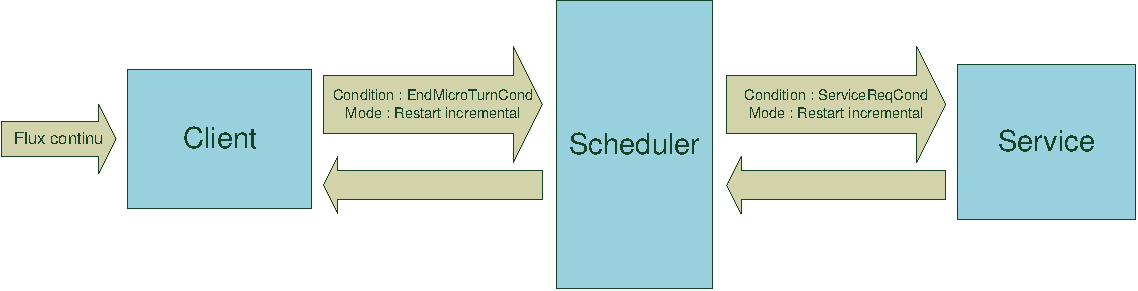
\includegraphics[scale=0.4]{figures/ClientSchedService.pdf}
          \caption{The Scheduler: an interface between the client and the service}
          \label{fig:archioverview}
        \end{figure*}
        
    \subsection{Time sharing}
    
    	In traditional dialogue systems, time is shared in an ordered and clear manner. The dialogue is a simple sequence of turns $T^1,T^2...$ a turn being the time interval in which a user's utterance followed by the system's corresponding response takes place, or the opposite (depending whether the system adopts a user initiative or a system initiative strategy at each turn). For illustration and to simplify the notation, the system used here is supposed to belong to the first category, therefore, each turn is divided into two smaller time intervals, the user turn $T^{k,U}$ and the system turn $T^{k,S}$: $T^k = T^{k,U} \cup T^{k,S}$ (the union of the time intervals corresponding to consecutive user and system turns, Figure \ref{fig:tradtimeshare}).
        
        In this chapter, a few conditions are defined to precisely describe time allocation between the system and the user. The \textit{activation time} of a condition refers to the exact moment when it goes from false to true. \textit{EndTurnCond} is the condition that ends a user turn, it is generally assimilated to a long silence \cite{Raux2008,Wlodarczak2013}.
        
        \begin{figure*}[t]
          \centering
          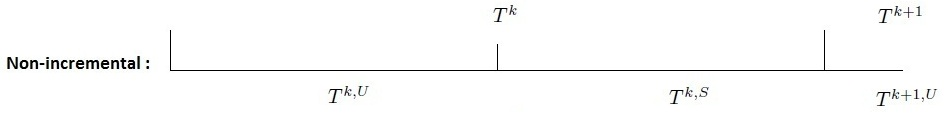
\includegraphics[scale=0.6]{figures/TraditionalTimeline.jpg}
          \caption{Time sharing in traditional settings}
          \label{fig:tradtimeshare}
        \end{figure*}

        \begin{figure*}[t]
          \centering
          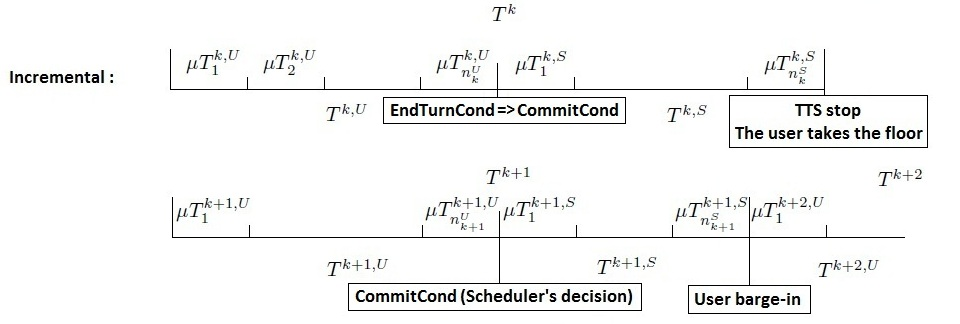
\includegraphics[scale=0.6]{figures/IncrementalTimeline.jpg}
          \caption{Time sharing in incremental settings}
          \label{fig:incrtimeshare}
        \end{figure*}
        
        In incremental settings, this time sharing formalism does not hold anymore and a new condition should be defined: \textit{EndMicroTurnCond} (with \textit{EndTurnCond} $\Rightarrow$ \textit{EndMicroTurnCond}). The time interval separating two activation times of \textit{EndMicroTurnCond} is called a \textit{micro-turn}. As a consequence, the turn $T^{k,U}$ can be divided into $n^{k,U}$ micro-turns $\mu T^{k,U}_i$: $T^{k,U} = \bigcup_{i=1}^{n^{k,U}} \mu T^{k,U}_i$. The $p^{th}$ \textit{sub-turn} of turn $T^{k,U}$ is defined as $T^{k,U}_p = \bigcup_{i=1}^p \mu T^{k,U}_i$ (Figure \ref{fig:incrtimeshare}).
        
        The request that the user makes during $T^{k,U}$ is referred to as $Req^k$ and the corresponding response is $Resp^k$. This architecture does not process incremental units like in \cite{Schlangen2011}, instead, at each new micro-turn, it will take the whole information available since the beginning of the turn\footnote{This way of managing incremental dialogue is called \textit{restart incremental} in \cite{Schlangen2011}.} (at the $p^{th}$ micro-turn, all what the user uttered during $T^{k,U}_p$). This \textit{partial request} is called $Req^k_p$.
        
    \subsection{The Scheduler}
    
    	\begin{figure*}[htp]
          \centering
          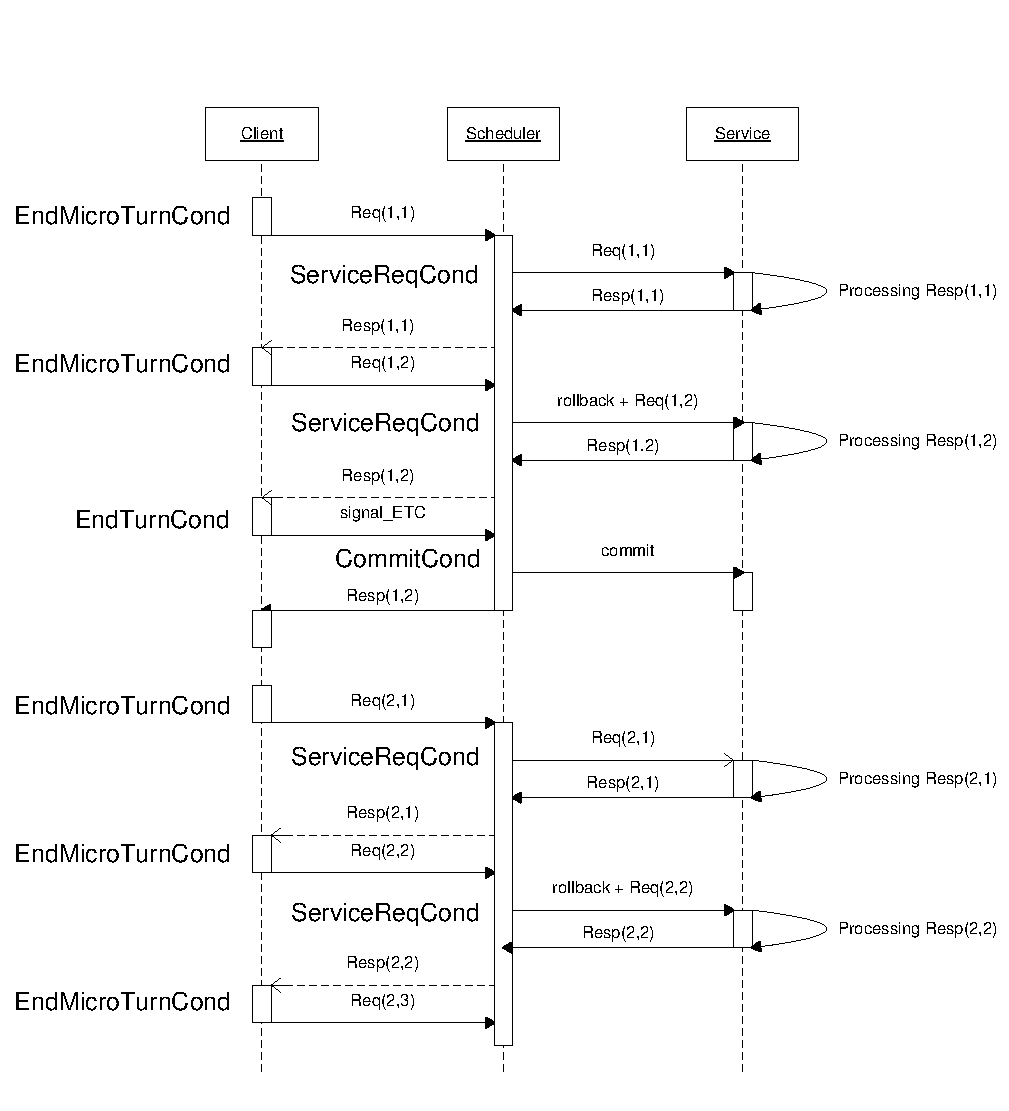
\includegraphics[scale=0.8]{figures/SchedulerDiagEng.pdf}
          \caption{Incremental request processing with the Scheduler: the conditions in the left column trigger the Client to send partial requests}
          \label{fig:schedchrono}
        \end{figure*}

	\begin{table*}[htp]
		\begin{center}
		\begin{tabular}{|c|c|c|c|c|}
			 \hline
			 \textbf{Turn} & \textbf{User sub-turn} & \textbf{Input} & \textbf{Real context} & \textbf{Simulation context} \\
			 \hline
			 $T^1$ & $T^{1,U}_1$ & $Req^1_1$ & ctxt($T^0$) & ctxt($T^0 + T^{1,U}_1$) \\
						 & $T^{1,U}_2$ & $Req^1_2$ & ctxt($T^0$) & ctxt($T^0 + T^{1,U}_2$) \\
						 &    ...     &     ...     & ctxt($T^0$) & ... \\
						 & $T^{1,U}_{n^{1,U}}$ & $Req^1_{n^{1,U}}$ & ctxt($T^0$) & ctxt($T^0 + T^{1,U}_{n^{1,U}}$) \\
			 \hline
						 & \multicolumn{3}{c}{\multirow{2}{*}{\textbf{COMMIT:} $ ctxt(T^1) = ctxt(T^0 + T^{1,U}_{n^{1,U}}) $}} & \\
						 & \multicolumn{3}{c}{} & \\
			 \hline
			 $T^2$ & $T^{2,U}_1$ & $Req^2_1$ & ctxt($T^1$) & ctxt($T^1 + T^{2,U}_1$) \\
						 &    ...     &     ...     & ctxt($T^1$) & ... \\
			 \hline
		\end{tabular}
	        \end{center}
	        \caption{A double context: the real context and the simulation context.}
	        \label{tab:contextchrono}
        \end{table*}
    
    	During the $p^{th}$ micro-turn of the $k^{th}$ user turn, the client sends $Req^k_p$ to the Scheduler. The latter has to decide whether to send it to the service or not and the corresponding condition is called \textit{ServiceReqCond}. A good example is \textit{ServiceReqCond} $\leftarrow$ ($Req^k_p \neq Req^k_{p-1}$) as sending the same brequest twice is useless. Then, the service provides the corresponding response $Resp^k_p$ and the Scheduler stores it. The key idea of this architecture is that the Scheduler decides whether to retrieve this response to the client (making it take the floor through the TTS) or not (waiting for more information to come from the client). This decision can also be forced by the client when sending an end of turn signal \textit{signal\_ETC}, like a long enough silence for instance. It is important to note that the Scheduler is able to decide when to take the floor without waiting for \textit{signal\_ETC}, the corresponding condition is called \textit{CommitCond}. The Scheduler functioning over time is illustrated in Fig. \ref{fig:schedchrono} (dashed arrows represent the Scheduler's response to the client since they may or may not take place, given the Scheduler's decision to commit or not).
                
        Nevertheless, this approach raises on technical problem. Most of the requests that are made to the service are only aimed to see what would be its response for certain partial utterances and they are discarded right after. However, they might modify the dialogue state in the service which is a side effect to be avoided. As a consequence, two dialogue contexts are maintained:
        
        \begin{itemize}
           	\item \textbf{The real context:} The dialogue context as traditionally used in dialogue systems. Contains the data and the variables that are aimed to last and be used in the rest of the dialogue.
        	\item \textbf{The simulated context:} A copy of the real context, at the $p^{th}$ micro-turn, $Resp^k_p$ could be useful for the dialogue or not. Therefore, only this context is modified at the first place, the Scheduler decides later whether to keep the changes in the real context or not.
        \end{itemize}
        
        These dialogue contexts are managed by two actions performed by the Scheduler:
        
        \begin{itemize}
        	\item \textbf{Commit:} The Scheduler commits to a partial request and the corresponding response when it decides to deliver the latter to the client, hence taking the floor immediately and not waiting for any further information. In that case, the simulated context is saved into the real context (thus becoming the new reference).
            \item \textbf{Cancel or rollback:} The scheduler cancels the context changes when it decides to discard the last response obtained from the service and that a new - potentially more complete - partial request is received from the client (as shown in Figure \ref{fig:schedchrono}). In that case, the real context is copied into the simulated one, rollbacking it to its original state.
        \end{itemize}
 
 		The way the real and the simulated context are managed through the commit and the cancel actions is illustrated in Table \ref{tab:contextchrono}.

        
\section{Illustration}

        As a proof of concept, this section describes two instanciations of the previous abstract architecture, both in the case of a textual and a spoken dialogue system.

	\subsection{A textual dialogue system: CFAsT}
    
    	\begin{figure*}[ht]
          \centering
          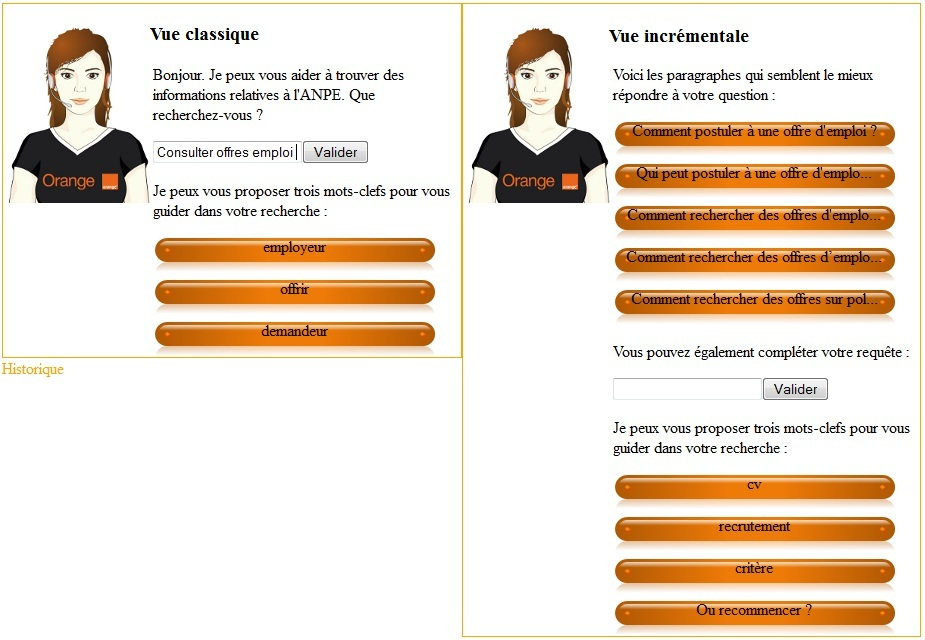
\includegraphics[scale=0.6]{figures/CFAsTIncr.jpg}
          \caption{The incremental version of the CFAsT project. The traditional view is represented on the left and the new incremental one is depicted on the left.}
          \label{fig:CFAsTIncr}
        \end{figure*}
        
        CFAsT stands for Content Finder AssistanT. This application, developed at Orange Labs \cite{Laroche2014,Laroche2015}, is aimed at automatically generating virutal assistants that help the user efficiently find specific content in databases (given as input). At each dialogue turn, the user provides some new information about his target and by using a keyword spotting algorithm, the system keeps narrowing the set of possibilites. The interface is made of a text box with a \textit{validate} button. The dialogue service is deployed as a web service on a servlet container and the client is a javascript web page loaded on the user's browser.
        
        In order to make it incremental, a Scheduler has been deployed as a servlet on the same container as the service and the javascript requests have been re-targeted towards it (the service is no longer directly visible by the client). Moreover, as discussed earlier, the dialogue context in the service have been duplicated. In this setup, \textit{EndTurnCond} corresponds to the event of clicking on \textit{validate} (or hitting the carriage return). A word-based micro-turn configuration has been implemented, therefore, \textit{EndMicroTurnCond} is the action of hitting the space bar. Each request being different from the previous one, they should all be sent to the service, thus, \textit{ServiceReqCond} is true all the time.
        
        This implementation is aimed to provide a first proof of concept of the methodology introduced here. However, signal\_ETC = \textit{CommitCond} = \textit{EndTurnCond} (the Scheduler never takes commit decisions by itself). The resulting behaviour presents a noteworthy similarity with autocompletion in search engines. The most staightforward way this mechanism is implemented is by continuously proposing several hypotheses regarding what would the complete request be, regarding the partial request typed so far. This does not require any request to the search engine itself (which can be viewed as the Service in the architecture introduced here). Another implementation (which lately started to be deployed) is by continuously updating the search result which is quite similar to what the transformed CFAsT achieves.
    
    \subsection{A spoken dialogue system: Dictanum}
    
    	Number dictation is an activity that can be encountered in several kinds of applicative domains: phone numbers, credit cards...Analysing human conversations in such situations shows that the number at hand is often broken into small pieces (a few digits each) and a confirmation follows each one of them. Therefore, the number is incrementally grounded so that in the case of a misunderstanding, only the last dictated part has to be repeated. Traditional dialogue systems behave differently as they ask the user to enter the whole number at once. This translates into long and tedious dialogues as only one minor mistake is enough to make the user repeat the number from the beginning, often for several times. For example:
        
        \begin{dialogue}
        	\speak{SYSTEM} Welcome to the Dictanum service. Please dictate your number.
            \speak{USER} 01 45 65 79 98.
            \speak{SYSTEM} The dictated number is 01 45 67 79 98. Is that correct?
            \speak{USER} No.
            \speak{SYSTEM} Sorry. Let us try again. Please dictate your number.
            \speak{USER} 01 45 65 79 98.
            \speak{SYSTEM} The dictated number is 01 47 65 79 98. Is that correct?
            \speak{USER} No.
            \speak{SYSTEM} Sorry. Let us try again. Please dictate your number. \\
            $\left[...\right]$ \textit{(given that the user is patient enough not to hang up)}
            \speak{SYSTEM} The dictated number is 01 45 65 79 98. Is that correct?
            \speak{USER} Yes.
            \speak{SYSTEM} Thank you for using Dictanum. Bye.
        \end{dialogue}
        
        With incremental dialogue processing, it is possible to design a strategy that is closer to the human behaviour. To show that, a number dictation dialogue system called Dictanum (described in \cite{Khouzaimi2014c})  has been implemented using Disserto. It performs turn-based dialogue hence asking the user for the whole number at once. Here, the client is a web page displayed on the browser that uses Google API for both the ASR and the TTS tasks and the service is a servlet deployed on a servlet container.
        
        Afterwards, the approach introduced here has been used to build the incremental version of the system (like in the case of the CFAsT application, the Scheduler has been deployed as a servlet on the same container as the service). To do so, two silence duration thresholds have been defined: the short silence threshold $\delta_s$ and the long one $\Delta_s$ ($\delta_s \leq \Delta_s$). \textit{EndMicroTurnCond} is triggered when a short silence is detected and similarly, \textit{EndTurnCond} corresponds to long silences. A feedback is delivered to the user in the case of a short silence (repeating the last 4 digits). If the user ignores the feedback and keeps dictating his number, the system keeps on adding digits to its list, however, if the user starts his next utterance with \textit{No}, the feedback content is deleted from the number. Here is a dialogue example:
        
        \begin{dialogue}
       	    \speak{SYSTEM} Welcome to the Dictanum service. Please dictate your number.
            \speak{USER} 01 45 \textit{(short silence)}
            \speak{SYSTEM} 01 45
            \speak{USER} 65 79 \textit{(short silence)}
            \speak{SYSTEM} 67 79
            \speak{USER} No, 65 79 \textit{(long silence)}
            \speak{SYSTEM} Sorry, 65 79
            \speak{USER} 98 \textit{(short silence)}
            \speak{SYSTEM} 98
            \speak{USER} ... \textit{(long silence)}
            \speak{SYSTEM} The dictated number is 01 45 65 79 98. Is that correct?
            \speak{USER} Yes.
            \speak{SYSTEM} Thank you for using Dictanum. Bye.
        \end{dialogue}

        It is interesing to notice that if $\delta_s = \Delta_s$, the user is likely to dictate his number in one shot, never waiting for a feedback. Therefore, moving $\delta_s$ between 0 and $\Delta_s$ creates a continuum between the traditional and the incremental version.
        
        Dictanum also offers the possibility for the user to interrupt the system during the final feedback, in order to make local corrections. To do that, this feedback is sent to the TTS in the following format: \textit{The dictated number is 01 <sep> 45 <sep> 65 <sep> 79 <sep> 98. Is that correct?}. The latter pronounces the sentence chunk after chunk (chunks are delimited using the separator \textit{<sep>}), each chunk lasting for the same number of micro-turns. This leads to the following kind of strategy:
        
        \begin{dialogue}
            \speak{SYSTEM} The dictated number is: 01 45 67...
            \speak{USER} No, 65.
            \speak{SYSTEM} Sorry. The dictated number is 01 45 65 79 98. Is that right?
            \speak{USER} Yes.
            \speak{SYSTEM} Thank you for using Dictanum. Bye.
        \end{dialogue}
    
\section{Discussion}

	\subsection{Levels of incrementality}
    
    	Dialogue systems can be classified in four categories given the way they integrate incremental behaviour. The first category is made of traditional systems \cite{CLASSiCd64}. Then comes the second category where traditional systems locally implements a few incremental behaviours. For instance, in \cite{El-Asri2014a}, the system enumerates a list of options and the user selects the one that fits him best by uttering \textit{Yes} or \textit{Ok} for example (REF\_RAW in the taxonomy introduced in Chap. \ref{ch:taxonomy}). The architecture introduced in this thesis belongs to the third category where incremental behaviour is obtained based on modules that are innately non-incremental (the service in our case). Other examples are described in \cite{Selfridge2012a} and \cite{Hastie2013}. Finally, the fourth category is made of incremental dialogue systems that are constituted of fully-incremental modules. In \cite{Schlangen2011}, an abstract model for incremental architectures is presented where all the categories can fit, but the work that has been pursued by the authors and their research groups later on goes along with the spirit of this last category.
		
		Categories 2, 3 and 4 embed different features related to incremental behaviour (summarised in Fig. \ref{tab:incrclassif}):

                \begin{itemize}
                  \item \textbf{TTS interruption after input analysis:} The user has the ability to interrupt the system (BARGE\_IN\_RESP from the user's side) but also to perform brief feedback (BACKCHANNEL or FEEDBACK TTP from the user's side) without interrupting the system's sentence. All categories except the first one can easily embed this feature.
                  \item \textbf{Link interruption time with TTS:} Useful for simulating REF TTP (REF\_IMPL, REF\_RAW and REF\_INTERP from the user's side). This has been successfully implemented in a system that belongs to the second category in \cite{El-Asri2014a}. Therefore, it can also be implemented in systems with a higher degree of incrementality (categories 3 and 4).
                  \item \textbf{User interruption by the system:} As it will be shown in the rest of this thesis, interrupting the user can improve the dialogue efficiency in some cases (BARGE\_- IN\_RESP from the system's side). To do so, the sytem at hand must offer real incremental capacities which is the case for categories 3 and 4 only.
                  \item \textbf{Better reactivity:} One of the main advantages of incremental processing is delivering responses in a quicker fashion since the processing of the user's request starts earlier. Again, real incremental abilities are required which makes it a property that is specific to categories 3 and 4 exclusively. This feature is particularly useful to achieve accurate end point detection (END\_POINT from the system's side).
                  \item \textbf{Optimal processing cost:} The third category processes the user's request in a restart incremental way (sending the whole partial utterance at each new micro-turn). This is not optimal as it is possible to process it chunk by chunk. Therefore, this is an advantage that category 4 offers over all the others.
                \end{itemize}

	\subsection{Enhancing a traditional dialogue system's turn-taking abilities at a low cost}
    
             Adopting the sequential paradigm described in Chapter \ref{ch:soadialogue} is a natural way of designing incremental dialogue systems \cite{Schlangen2011}. The dialogue chain is kept unchanged, however, a substantial amount of work has to be done in order to design an incremental version of each one of the modules. The approach introduced in this chapter makes it possible to build an incremental dialogue system starting from a traditional one instead of starting from scratch. Therefore, the development cost is significantly reduced and moreover, the resulting incremental dialogue system benefits from all the experience and the adjustments embedded in the original dialogue system. In the following, the differences between the two approaches are reviewed as well as the elements that are simplified with the new approach and the price one has to pay to adopt it.

             Incremental ASR is a prerequisit for the implementation of a Scheduler-based architecture. Therefore, it is not simplified by this approach and an inaccurate, slow or unstable ASR module still hurts the dialogue quality in the same way. In terms of NLU, two cases have to be distinguished: putting the Scheduler before the NLU or after it. In the first case, it does not make sense to use an incremental NLU as the Scheduler proceeds on a restart incremental fashion (sending the whole user's partial utterance at each micro-turn). However, in the second case, it is possible to benefit from the advantages of incremental NLU (forming concepts in a real incremental way resulting in more efficient processing). In that case, the Scheduler receives a sequence of potentially unstable sets of concepts.

             The core difference between both approaches resides in the DM task. In a full-incremental architecture, dialogue act and turn-taking decisions are intertwined. The DM receives the input concepts chunk by chunk, and at each micro-turn, the new information can be viewed as the continuity of what has been understood so far, or as a signal pushing the DM to revoke the current hypothesis before taking a new action. In the Scheduler-based approach, as the restart incremental paradigm is adopted, the revoke mecanism is intrinsicly implemented as it is performed beforehand (the ASR changing its best hypothesis is a case of revoke).

             Incremental NLG does not make sense in the frame proposed here as the Scheduler can only retrieve full dialogue acts that have been precomputed by the service. As a consequence, the system can change its mind about the utterance currently uttered but it can only generate a new dialogue act from scratch with is potentially not related to the previous one. Nevertheless, as discussed in Chapter \ref{ch:soadialogue}, this is not a major problem when it comes to spoken dialogue systems relying on voice as the only interaction modality. It is mostly used when the system produces comments about a moving object or situation it is observing \cite{Baumann2013}.

             Finally, as far as the TTS task is concerned, the same remark as for the NLG can be made. However, it can be interesting to give the Scheduler the power to stop the TTS. This is particularly interesting when the DM decides to revoke its current belief.

             \begin{table*}[!ht]
      	     \footnotesize
             \centering
             \begin{tabular}{|c|c|c|c|c|}
               \hline
               \textbf{Features}	& \textbf{Category 1} & \textbf{Category 2} & \textbf{Category 3} & \textbf{Category 4} \\
               \hline
               TTS interruption after input analysis & - & + & + & + \\
               \hline
               Link interruption time with TTS & - & + & + & + \\
               \hline
               User interruption by the system & - & - & + & + \\
               \hline
               Better reactivity & - & - & + & + \\
               \hline
               Optimal processing cost & - & - & - & + \\
               \hline
             \end{tabular}
             \caption{Available features for dialogue systems given the way they integrate incrementality}
             \label{tab:incrclassif}
             \end{table*}

\chapter{Incremental dialogue simulation}
\label{ch:simulation}

	% In this chapter, a new simulated environment is introduced. It is based on an incremental dialogue system based on the methodology presented in Chapter \ref{ch:architecture} as well as a new incremental dialogue User Simulator (US) that is able to interact with it. The novelty of the latter is that it is able to simulate the ASR instability phenomenon.
	
	Using dialogue simulation techniques is very common in the research community \cite{Eckert1997,Pietquin2006} for several reasons like: the ability to quickly generate dialogue corpora that can be used to develop machine learning techniques, an easy way to model different populations of users and the possibility to use the same user simulator to test and compare concurrent dialogue strategies (see Chapter \ref{ch:soarl} for more details). In this chapter, a new incremental dialogue simulation framework is introduced (published is \cite{Khouzaimi2016a}). Its novelty resides in the fact that it is able to simulate the ASR instability phenomenon. First, it is presented in its most generic and abstract form that can be used by the reader to instantiate his/her own simulator that is adapted to any target domain. Then, these principles are applied in order to implement a showcase simulated environment where the service is a personal agenda manager.
	
	Later on, this simulated environment is used for two main purposes. Firstly, the slot-filling and the incremental dialogue strategies described in Chapter \ref{ch:strategies} are implemented and compared. This somehow validates the preliminary efficiency analysis led in that chapter. It also provides new analysis elements to go further and prepare a basis for the experiments with real users. Secondly, it is a very useful tool for generating data to train machine learning algorithms. In Chapter \ref{ch:rl}, it is used to train a reinforcement learning algorithm which purpose is to optimise turn-taking decisions.
						
\section{Overview}
	
	How to run dialogues with no users? The well-known answer is: by designing a User Simulator (US). Rigorously, in the case of SDSs, a US should be able to process an input audio signal and to output a new audio signal as well. Even though this method has its merits (noise and ASR imperfections are naturally taken into account), it goes against one of the main advantages of user simulation techniques which is the ability to quickly generate an important number of dialogues. Also, making an ASR module listen to a TTS and understand its message is not easy. Therefore, the user simulator elaborated here inputs and outputs text. An ASR output simulator is in charge of replicating the ASR behaviour. Figure \ref{fig:simuoverview} gives an overview of how these parts fit together in the whole architecture as well as the composition of the US. The latter is composed of five modules: The Intent Manager, the NLU, the Verbosity Manager, the NLG and the Patience Manager.
	
		\begin{figure*}[htb]
			\centering
			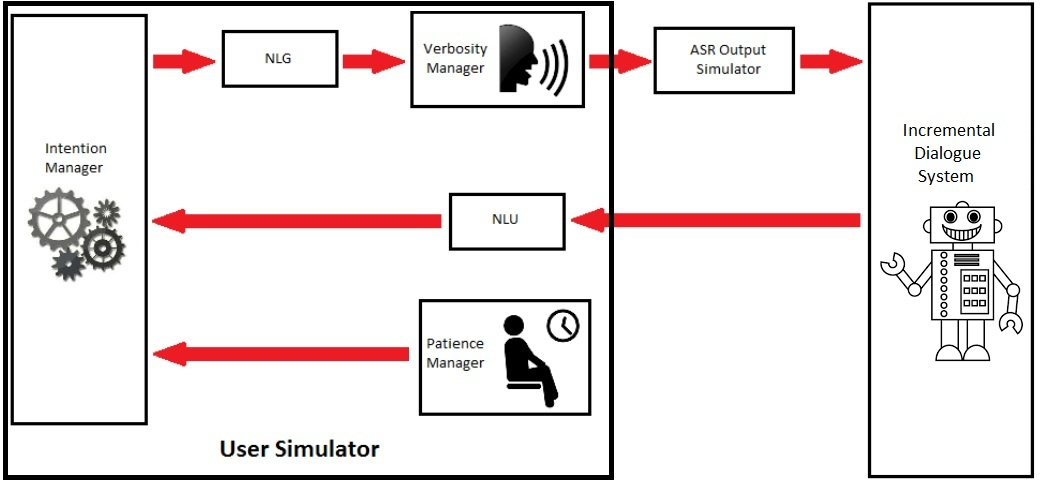
\includegraphics[scale=0.45]{figures/SimuSys.jpg}
			\caption{Simulated environment architecture}
			\label{fig:simuoverview}
		\end{figure*}
    
\section{Incremental dialogue simulation}
				
				In a nutshell, at the $p^{th}$ micro-turn of the $k^{th}$ user turn $\mu T^{k,U}_p$, the US generates a partial utterance $Req^k_p$ that is transformed into an N-Best ${(score^k_{p,1}, hyp^k_{p,1}),...,(score^k_{p,N}, hyp^k_{p,N})}$, which corresponds to the N recognition hypotheses that have the best confidence scores. It corresponds to the whole utterance pronounced during the partial turn $T^{k,U}_p$ (\textit{restart incremental} mode \cite{Schlangen2011}). On the other hand, either the US receives an answer from the dialogue system at a certain micro-turn and it stops speaking\footnote{This is of course an approximation of real barge-in cases since the overlap is neglected.}, either it does not and it continues speaking if it has additional things to say (releasing the floor otherwise). When the dialogue lasts for too long without achieving the task at hand, the US can end the dialogue.

                                In the following, the role and the functioning of the US and the ASR output simulator is discribed in an abstract fashion before being instanciated later on to give birth to a personal agenda management simulated environment.
    
	\subsection{User Simulator}

			\subsubsection{Intent Manager}
			\label{subsec:intentmanager}

					The Intent Manager is in charge of computing the dialogue acts that the US performs. It maintains an internal dialogue context and takes the dialogue acts coming from the dialogue system as inputs. Thus, it can be viewed as a dialogue manager in itself but with the difference that it is aimed to generate requests and to lead the dialogue instead of serving a user (at least in task-oriented situations). Therefore, it is given a task or a list of tasks to accomplish before it starts interacting with the dialogue system.

					A common approach to design such a module is the agenda-based method \cite{Wei1999,Schatzmann2007}. Inspired by the latter, the approach adopted in this thesis suggests that the tasks the Intent Manager should accomplish are given in the form of a stack (LIFO structure): the action stack (AS). They are removed and executed one by one and during each step, new actions could be added. The Algorithm \ref{algo:abstractim} describes a function called \textit{run} with AS as an argument and that is in charge of unstacking all the corresponding actions and executing them by using the method \textit{perform()}. The latter tries to execute the top element of the action stack which might lead to the removal of the top element of the stack or the creation of new actions that are added on top of AS (which justifies the fact that the whole stack is passed as an argument and not the top element only). A loop is run over the elements of AS until it is empty.

					\begin{algorithm}[htp]
						\DontPrintSemicolon
						\SetKwFunction{run}{run}
						\SetKwProg{myalg}{Algorithm}{}{}
						\myalg{\run{AS}}{
							\While{AS.size > 0}{
								perform(AS);
							}
						}
						\caption{Intent Manager abstract algorithm}
						\label{algo:abstractim}
					\end{algorithm}

			
			\subsubsection{NLG and Verbosity Manager}
				
				The NLG module of the simulator transforms the Intent Manager's output into a simple and straightforward utterance. For example:
				
				\begin{itemize}
					\item Book a room for tomorrow.
					\item Record channel 2 from 6pm until 8pm.
					\item Delete the event football game from the agenda.
				\end{itemize}
				
				Compared to human/human conversations, limiting interactions to this kind of simple utterances is not realistic. Therefore, they are enhanced in the Verbosity Manager with prefixes like \textit{I would like to}, \textit{Is it possible to}...and suffixes like \textit{if possible}, \textit{please}... In \cite{Ghigi2014}, a corpus study showed that users tend to go off-domain and to repeat the same information several times in the same sentence. These behaviours are also replicated in the Verbosity Manager: with a probability $p_{od}$ the NLU output is replaced with an off-domain sentence randomly picked in a predefined list, moreover, with a probability $p_{rep}$ and given that the system just reported a misunderstanding, the utterance is repeated twice (for example, \textit{Check my account, I repeat, check my account}).
			
			\subsubsection{Timing and patience manager}
			
				When it comes to incremental processing, timing is key. However, the main objective of simulation is to generate dialogues as fast as possible, hence, real time stamps cannot be used. In order to approximate durations, the user's and the system's speech rates are considered to be constant with value $SR$.
					
					Users tend to get impatient, at various degrees, when dialogue systems take too long to accomplish the task they are asked for. To simulate this behaviour, a duration threshold is chosen at each new dialogue that will cause the user to hangup as soon as it is reached. It is computed as follows
					
					\begin{eqnarray}
						d_{pat} = 2 \mu_{pat}.sigmoid(X)
					\end{eqnarray}
					
					where X follows a Gaussian distribution of mean 0 and variance 1 and $\mu_{pat}$ is the mean duration since
					
					\begin{eqnarray}
						sigmoid(x) & = & \frac{1}{1 + e^{-x}}
					\end{eqnarray}
					
					
	\subsection{ASR output simulator}
			
				The ASR output simulator generates an N-Best that is updated at each new micro-turn. For instance, if at a certain point, the US uttered \textit{I would like to add the event birthday party on...}, a possible N-Best could be (the numbers between brackets represent ASR scores):
					
					\begin{itemize}
						\item (0.82) I would like to add the event birthday party on
						\item (0.65) I like to add the event birthday party on
						\item (0.43) I have had the event birthday party
						\item (0.33) I would like to add the holiday party
						\item (0.31) I like to add the holiday party on
					\end{itemize}
					
					More formally, at the $p^{th}$ micro-turn of the $k^{th}$ user turn $\mu T^{k,U}_p$, the N-Best is an N-uplet ${(score^k_{p,1}, hyp^k_{p,1}),...,(score^k_{p,N}, hyp^k_{p,N})}$. At time t+1, a new word $w_{t+1}$ is sent to the ASR output simulator and the latter calculates a new associated N-Best. Therefore, at this stage, the system has two N-Bests:
					
					\begin{itemize}
						\item \textbf{The word N-Best:} It corresponds to the different hypotheses related to the last word pronounced. In Figure \ref{fig:asrsimu}, the top right box represents the word N-Best associated with the word $6^{th}$.
						\item \textbf{The utterance N-Best:} It designates the N-Best associated with the whole partial utterance pronounced so far. In Figure \ref{fig:asrsimu}, the top left box is an a example of such N-Best associated with the partial utterance \textit{I want to add the event birthday party on January}.
					\end{itemize}
					
					Both are combined to form the new utterance N-Best. In the following, the way the word N-Best is calculated and the way it is incorporated into the partial utterance N-Best are described.
					
					In order to simulate noise and ASR imperfections, the ASR output simulator uses a module called the Scrambler. It receives a word as input and performs one of the three following operations in order to compute the output\footnote{The Scrambler always performs one these three operations. In other words $p_{repl} + p_{add} + p_{del} = 1$}:
					
					\begin{itemize}
						\item Replace the word with a different word taken randomly from a dictionary (probability: $p_{repl}$)
						\item Add a new word (probability : $p_{add}$)
						\item Delete the word (probability : $p_{del}$)
					\end{itemize}
					
					A Word Error Rate (WER) is given as a parameter to the ASR output simulator. It controls the noise level that one wants to simulate. The algorithm used to generate the N-Best associated with a single word is described below:
					
					\begin{figure}[t]
					\centering
					\begin{tikzpicture}[scale=0.8]
					\begin{axis}[
						xlabel={Confidence score},
						ylabel={Density},
						scaled ticks = false,
						tick label style={/pgf/number format/fixed},
						xmin=0, xmax=1,
						ymin=0, ymax=0.55,
						xtick={0,0.2,0.4,0.6,0.8,1},
						ytick={0.1,0.2,0.3,0.4,0.5,0.6},
											legend pos=north east,
						ymajorgrids=true,
						grid style=dashed,
											colorbrewer cycle list=Set2,
					]
					
					\addplot+[
						error bars/.cd,
						y dir=both,
						y explicit,
						]
						coordinates {
						(0,0)
	(0.1,0.19483312081792062)
	(0.2,0.3702598583755481)
	(0.3,0.3943180330023535)
	(0.4,0.33431406881442405)
	(0.5,0.24197072451914337)
	(0.6,0.1485840305841884)
	(0.7,0.07242576116369753)
	(0.8,0.023141241148471745)
	(0.9,0.00240534717059161)
	(1,0)
						};
											
											\addplot+[
						error bars/.cd,
						y dir=both,
						y explicit,
						]
						coordinates {
						(0,0)
	(0.1,0.002405347170591614)
	(0.2,0.023141241148471745)
	(0.3,0.0724257611636976)
	(0.4,0.14858403058418854)
	(0.5,0.24197072451914337)
	(0.6,0.33431406881442416)
	(0.7,0.3943180330023536)
	(0.8,0.37025985837554803)
	(0.9,0.1948331208179205)
	(1,0)

						};
											

					\legend{Bad recognition,Good recognition}

					\end{axis}
					\end{tikzpicture}
					\caption{ASR score sampling distribution ($\sigma_{conf} = 1$)}
					\label{fig:scoresample}
			\end{figure}
			
					\begin{enumerate}
						\item Determine whether $w_{t+1}$ is among the N-Best or not with a probability that is computed as follows: (1 - WER) + INBF.WER, where INBF (In N-Best Factor) is a parameter between 0 and 1. If $w_{t+1}$ is not in the N-Best, then the latter contains only scrambled versions of this word and jump to step 4.
							\item The first hypothesis is set to be $w_{t+1}$ with a probability of (1-WER), otherwise, it is a scrambled version of it.
							\item If the the first hypothesis is not $w_{t+1}$, then this word's position is randomly chosen between 2 and N. Moreover, the other hypotheses are scrambled versions of it.
							\item The confidence score associated with the best hypothesis ($score_0$) is sampled as sigmoid(X) where X follows a Gaussian distribution. More precisely,\\$X \sim \mathcal{N} (c_{err},\sigma_{conf})$ if the first hypothesis is wrong and $X \sim \mathcal{N} (c_{right},\sigma_{conf})$ when it is right (with $c_{err} < 0 < c_{right}$). By taking the sigmoid, this leads to two distributions\footnote{Confidence score estimation is a complex problem and it is still a research topic \cite{Jiang2005,Seigel2011}. The simple model introduced here is inspired by \cite{Pietquin2005}. Also, notice that the scores are between 0 and 1 but they do not sum up to 1 since they are not probabilities.} (depicted in Figure \ref{fig:scoresample} for $\sigma_{conf} = 1$) with a mean on both sides of 0.5 and the same standard deviation for both (which is a growing function of $\sigma_{conf}$ and which can be changed to simulate different levels of accuracy of the confidence score model). Big $\sigma_{conf}$ values lead to spread recognition scores and small differences between $c_{err}$ and $c_{right}$ engender close scores for both cases: right and wrong first hypothesis. Therefore, discriminative models are obtained for small values of $\sigma_{conf}$ and high difference $c_{right}-c_{err}$.
							\item The scores for the other hypotheses are computed in an iterative way. For $i$ between 2 and N, $score_i$ is uniformly sampled in $[0,score_{i-1}]$.
					\end{enumerate}
					
					As already mentioned in this thesis, early partial utterances are not necessarily prefixes of later ones with a true ASR system (ASR instability phenomenon). To replicate this behaviour, a language model is needed to compute the scores corresponding to the different hypotheses in the N-Best. Therefore, sentences that are more in alignment with the model have higher scores thus being pushed to the top of this N-Best. Here, the NLU knowledge is used as a proxy for the language model by making the following assumption: \textit{the more an utterance generates key concepts once fed to the NLU, the more it is likely to be the correct one}. Therefore, as soon as a new concept is detected in $hyp^k_{p,i}$, $score^k_{p,i}$ is boosted as follows:
					
						$$ score^k_{p,i} \leftarrow score^k_{p,i} + BF.(1 - score^k_{p,i}) $$
							
					where BF is the Boost Factor parameter. An illustration of this mechanism with BF=0.2 is provided in Fig. \ref{fig:asrsimu}.
					
					\begin{figure*}[h]
						\centering
						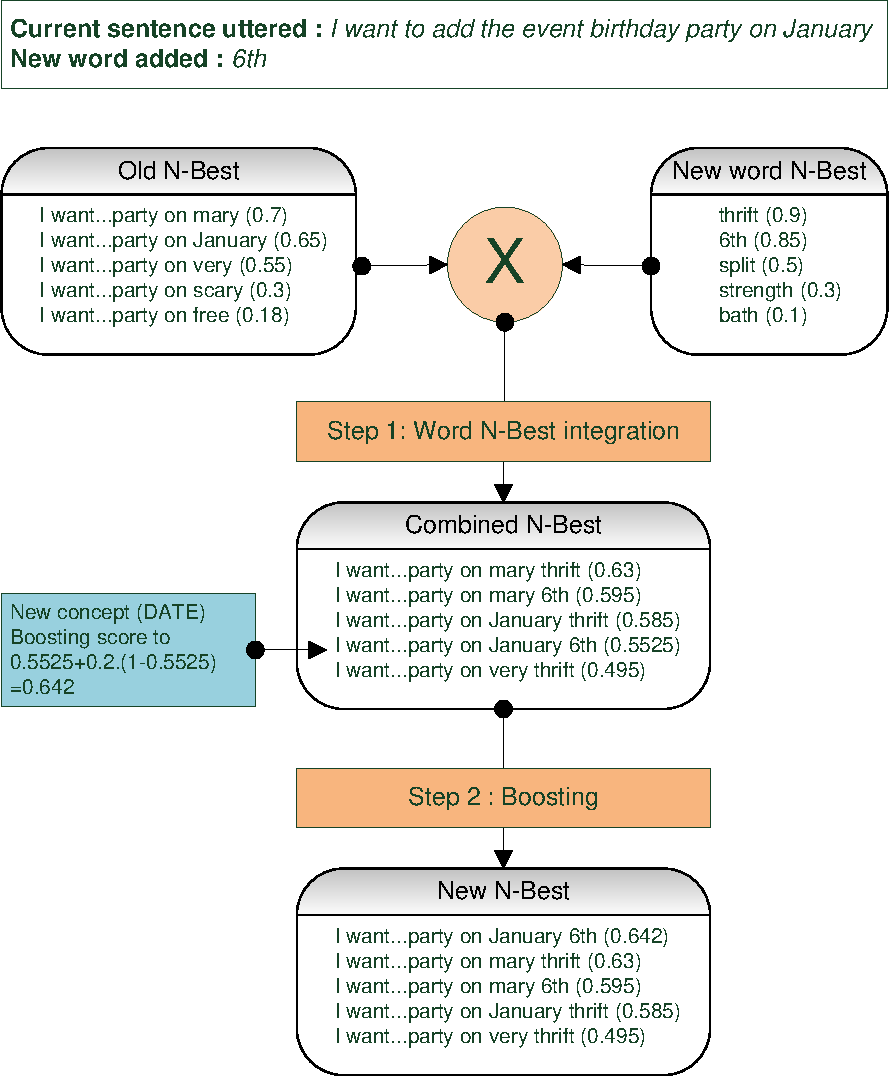
\includegraphics[scale=0.75]{figures/ASRSimu.pdf}
						\caption{An illustration of the incremental ASR output N-Best update (BF=0.2)}
						\label{fig:asrsimu}
					\end{figure*}

\section{Personal Agenda management simulated environment}

	So far, an abstract framework for simulating incremental dialogues has been described. In this section, it is instanciated to be able to generate dialogues with an incremental dialogue system which purpose is to help users manage their personal agenda. This task will be used in Chapter \ref{ch:baseline} in order to run a few experiments regarding the dialogue strategies introduced in Chapter \ref{ch:strategies} and in Chapter \ref{ch:rl} to test a new reinforcement learning approach. First the Service (system side, Section \ref{subsec:service}) and its dialogue task are presented, then the way the US (user side, Section \ref{subsec:us}) and the ASR output simulator are instanciated is described.
	
	\subsection{The Service: personal agenda assistant}
        \label{subsec:service}
	
		\subsubsection{Dialogue Manager}

			A personal agenda assistant has been implemented as a new task for the experiments. The user can add, move or delete events in his agenda. For instance, a request could be: \textit{I would like to add the event football game on March $3^{rd}$ from 9 to 10 pm}\footnote{The dialogues are actually in French but they are translated in English to ensure language coherence in this thesis.}. This is a slot-filling task with four slots:
				
				\begin{itemize}
					\item \textbf{ACTION:} The type of action the user wants to perform. Can take three different values: ADD, MODIFY or DELETE.
						\item \textbf{DESCRIPTION:} The description of the event.
						\item \textbf{DATE:} The date of the event.
						\item \textbf{WINDOW:} The time window of the event.
				\end{itemize}
				
				However, no overlap is tolerated between events in the agenda.
				
				Each interaction between the US and the system is defined by a scenario. Here, the US is given two lists of events: \textit{InitList} and \textit{ToAddList}. The first one contains the events that already exist in the agenda before the dialogue and the second one contains the ones that the US is supposed to add during the dialogue. Each event is associated with a priority value and the US must prefer adding the ones with high priority first\footnote{To make the algorithms easier to understand, the larger priority value, the more important the event, unlike common usage.}. Its aim is to make as many events with the highest priority values as possible fit in the agenda.
				
		
		\subsubsection{Natural Language Understanding}
		
			A rule-based algorithm transforms the user's utterance hypothesis into concepts. To do that, a set of rules have been defined. Each rule transforms a word, a concept or any combination of the two into a new concept. Three types of rules are used; they are depicted in Table \ref{tab:ruletypes}.
			
			For instance, parsing the sentence \textit{I want to add the event birthday party on January $6^{th}$ from 9pm to 11pm} is performed following these steps:
							
							\begin{enumerate}
						\item \textbf{I want to ADD the TAG\_EVENT birthday party on MONTH(January) NUMBER(6) from TIME(9,0) to TIME(11,0)}
								\begin{itemize}
										\item add : [ADD]
											\item event : [TAG\_EVENT]
											\item Regex(janvier|...|decembre) : MONTH(\$word)
											\item Regex([0-9]+) : NUMBER(\$word)
											\item Regex((([0-1]?[0-9])|(2[0-3]))h([0-5][0-9])?) : TIME(\$word)\footnote{Adapted to the french way of uttering time values.}
									\end{itemize}
							\item \textbf{I want to ADD the TAG\_EVENT birthday party on DATE(6,1) \\ WINDOW(TIME(21,0),TIME(23,0))}
								\begin{itemize}
										\item Combine(NUMBER,MONTH) : DATE(NUMBER,MONTH)
											\item Combine(from,TIME\_1,to,TIME\_2) : WINDOW(TIME\_1,TIME\_2)
									\end{itemize}
							\item \textbf{I want to ADD EVENT(birthday party, DATE(6,1), \\ WINDOW(TIME(21,0),TIME(23,0)))}
								\begin{itemize}
										\item Combine(TAG\_EVENT,\$x,on,DATE,WINDOW) : EVENT(\$x,DATE,WINDOW)
									\end{itemize}
							\item \textbf{I want ACTION(ADD, EVENT(birthday party, DATE(6,1), \\ WINDOW(TIME(21,0),TIME(23,0))))}
								\begin{itemize}
										\item Combine(ADD,EVENT) : ACTION(ADD,EVENT)
									\end{itemize}
					\end{enumerate}
					
			\subsection{Simulator instanciation}
                        \label{subsec:us}
			
				\begin{table}[t]
					\fontsize{8}{10}\selectfont
					\vspace{2mm}
					\centerline{
						\begin{tabular}{|l|l|l|}
							\hline
							\textbf{Rule type} & \textbf{Description} & \textbf{Example} \\
							\hline
							Tag & Words are associated with labels & remove : [DELETE] \\
							Regular expressions & Words matching a regular expression & Regex([0-9]+) : NUMBER(\$word) \\
							& are transformed into concepts & \\
							Combine & Words and concepts are mapped into a new concept & Combine(NUMBER,MONTH) : DATE \\
							\hline
						\end{tabular}
					}
					\caption{\label{tab:ruletypes} {NLU rules types}}
				\end{table}
			
				\begin{algorithm}[htp]
					\DontPrintSemicolon
					\SetKwRepeat{Do}{do}{while}
					\SetKwFunction{run}{run}
					\SetKwProg{myalg}{Algorithm}{}{}
					\myalg{\run{AS}}{
						\While{AS.size > 0}{
							altQ $\gets$ AS.top.event.alt\;
							c $\gets$ empty map\;
							M $\gets$ empty map\;
							\Do{altQ.size > 0 AND conflQ.size > 0}{
								conflQ $\gets$ execute((AS.top.action,altQ.next))\;
								\If{conflQ.size > 0}{
									c.add(altQ.next,conflQ)\;
									M.add(altQ.next,$\max_{e \in \text{conflQ}}$ e.prio)\;
									altQ.removeNext()\;
								}
							}
							\eIf{conflQ.size > 0}{
								$e_{best} \gets$ argmin(M)\;
								\eIf{M($e_{best}$) < AS.top.event.prio}{
									\For{e $\in$ c($e_{best}$)}{
										\eIf{e.alt.size > 1}{
											\For{e' $\in$ e.alt-\{e\}}{
												AS.add((MOVE,e'))\;
											}
										}{
											AS.add((DELETE,e))\;
										}
									}
								}{
									AS.removeTop()\;
									\If{AS.top.action == MOVE}{
										AS.add((DELETE,AS.top.event))\;
									}
								}
							}{
								AS.removeTop()\;
							}
						}
					}{}
					\caption{Intent Manager algorithm}
					\label{algo:intent}
				\end{algorithm}
			
				\begin{table}[htp]
						\fontsize{8}{10}\selectfont
						\vspace{2mm}
						\centerline{
							\begin{tabular}{|l|l|l|}
								\hline
								\textbf{Parameters} & \textbf{Value} & \textbf{Justification} \\
								\hline
								$p_{od}$ & 0.1 & Based on the corpus study led in \cite{Ghigi2014} \\
								$p_{rep}$ & 0.3 & Id. \\
								$SR$ & 200 words per minute & See \cite{Yuan2006} \\
								$\mu_{pat}$ & 3 min & Empirical given the task \\
								$p_{repl}$ & 0.7 & Empirical (variable and difficult to estimate) \\
								$p_{add}$ & 0.15 & Id. \\
								$p_{del}$ & 0.15 & Id. \\
								N & 5 & Empirical (can be anything depending on the ASR configuration) \\
								INBF & 0.7 & Tuned for a reasonable boosting effect with N=5 \\
								BF & 0.2 & Id. \\
								$c_{err}$ & -1 & Empirical (variable and difficult to estimate) \\
								$c_{right}$ & 1 & Empirical (variable and difficult to estimate) \\
								$\sigma_{conf}$ & 1 & Id. \\
								SM & 2 & words that lasted for more than 0.6 seconds have 90\% chance \\
								& & of staying unchanged \cite{McGraw2012} \\
								& & and SR = 200 wpm \\
								WER & Variable during the experiments & \\
								\hline
							\end{tabular}
						}
						\caption{User simulator and ASR output simulator values}
						\label{tab:paramvalues}
					\end{table}
			
				The aim of the US is to make the biggest number possible of events with the highest priority values taken from \textit{InitList} and \textit{ToAddList} fit in the agenda. To do so, the Intent Manager executes the \texttt{run()} function (taking the action stack (\texttt{AS}) as an argument) depicted in Algorithm \ref{algo:intent} (an instance of the abstract function depicted in Algorithm \ref{algo:abstractim}) where
				
				\begin{itemize}
					\item The manipulated structures are stacks and queues.
					\item If \texttt{st} is a stack, the top element is called \texttt{st.top} and \texttt{st.removeTop()} removes it from \texttt{st}.
					\item If \texttt{q} is a queue, the next element is called \texttt{q.next} and \texttt{q.removeNext()} removes it from \texttt{q}.
					\item The size of the structure \texttt{x} is called \texttt{x.size}.
					\item If \texttt{m} is a map, \texttt{m.add(x,y)} adds a new entry to m such that \texttt{m(x) = y}.
					\item \texttt{AS} is a stack of actions and each action a is a couple (\texttt{a.action},\texttt{a.event}) where \texttt{a.action} is an action type (ADD, MODIFY or DELETE) and \texttt{a.event} is an event caracterised by a description, a date, a time window and a priority value.
					\item For each event \texttt{e}, \texttt{e.alt} refers to all its alternatives including itself\footnote{The elements of \texttt{e.alt} share the same description and priority value but they have different dates and time windows.}. Its priority is called \texttt{e.prio}.
					\item The function \texttt{execute()} communicates an intent to the NLG and gets the corresponding response through the NLU. If this response is a misunderstanding declaration, then the same intent is sent again. If it is a declaration of conflict with a set of other events, then a queue with all these events is returned. Finally, if no conflict was detected, then this function returns an empty queue. This is how the US updates \texttt{AS}.
				\end{itemize}
						
					The other parameters of the US and the ASR output simulator are set as shown in Table \ref{tab:paramvalues}.
					
\section{Functionning illustration}
			
				The following illustration provides the reader with a global view of all the notions introduced in this chapter through an application to a concrete interaction in the agenda management domain. Consider the following scenario:
				
				\begin{itemize}
					\item \textbf{InitList:} \{\textbf{title:} \textit{house cleaning}, \textbf{date:} \textit{January $6^{th}$}, \textbf{window:} \textit{from 18 to 20}, \textbf{priority:} \textit{3}, \textbf{alternative 1:} \textit{January $7^{th}$, from 6pm until 8pm}, \textbf{alternative 2:} \textit{January $9^{th}$, from 10am until 12am}\}
					\item \textbf{ToAddList:} \{\textbf{title:} \textit{birthday party}, \textbf{date:} \textit{January $6^{th}$}, \textbf{window:} \textit{from 6pm until 11pm}, \textbf{priority:} \textit{5}\}
				\end{itemize}
				
				\texttt{AS} initially contains the ADD action associated with the event \textit{birthday party} since it is the only event in \textit{ToAddList}. Let \texttt{e} be this event. The function \texttt{run()} in Algorithm \ref{algo:intent} is then run over this stack. Thus the first result generated by the Intent Manager is the ADD action corresponding to the event \textit{birthday party}. Once communicated to the NLG, the latter outputs the sentence \textit{Add the event birthday party on January $6^{th}$ from 6pm until 8pm} which is in turn transfered to the Verbosity Manager. $p_{od}=0.1$ so there is a 10\% chance that the result of the NLG is ignored and replaced by an off-domain sentence. Suppose it is the case for this first trial then the ASR output simulator's result is also off-domain. As a consequence, the service responds by saying that the user's requests has not been understood which is recognised as a dialogue act by the NLU and communicated to the Intent Manager. The function \texttt{execute()} then sends the same intent once again to the NLG which generates the same utterance as it did the first time. As the last system's response is a misunderstanding declaration, the Verbosity Manager has $p_{rep}=0.3$ chance of repeating the same sentence twice. Suppose it is the case, then the Verbosity Manager's output is the following (a prefix and a suffix are also randomly added by this module): \textit{Can you please add the event birthday party on January $6^{th}$ from 6pm until 8pm, I repeat, add the event birthday party on January $6^{th}$ from 6pm until 8pm if it is possible}. The ASR output simulator generates an N-Best as it is described in Figure \ref{fig:asrsimu}.
				
				Suppose that \textit{CommitCond} in the Scheduler is true if and only if the response to the last stable utterance is either a confirmation question or a conflict declaration (in other words, all the slots have been successfully communicated to the system). Also, suppose that this time, the best ASR hypothesis is 100\% correct. Since SM=2, the Scheduler decides to take the floor as soon as the users decides to utter \textit{Can you please add the event birthday party on January $6^{th}$ from 6pm until 8pm, I repeat}.
				
				Since the time window required to organise the birthday party is already taken by the house cleaning event \texttt{execute()} returns a queue (\texttt{conflQ}) containing the latter only, and the entry (\texttt{e},\texttt{conflQ}) is added to \texttt{c}. The priority of the house cleaning event is 3, therefore, the entry \texttt{(e,3)} is added to \texttt{M}. Therefore, $e_{best} =$ \texttt{e} since it is the only element in \texttt{M}. Its priority is lower than \texttt{AS.top.event.prio}. As a consequence, the Intent Manager tries to move the house cleaning event (details about the sentence formulation and management are no longer given) and it ends up to be successful using the first alternative: \textit{January $7^{th}$, from 6pm until 8pm}. By doing so, the event \textit{birthday party} is still in the stack and it is added facing no problem this time since the corresponding time window has been freed.

                                To sum up, a new incremental dialogue simulation which supports dialogue instability has been introduced in detail in this chapter. Its different components have been thoroughly described as well as the way they interact with each other to incrementally send requests to the system and to process its responses. In the rest of this thesis, the strategies formerly described are implemented and evaluated in this simulated environment, then the latter is used to train a reinforcement learning turn-taking strategy.

\chapter{Handcrafted strategies for improving dialogue efficiency}
\label{ch:baseline}

	Several strategies for handling slot-filling dialogue tasks have been discussed in Chapter \ref{ch:strategies}. The hypothesis laid stipulates that they perform differently under different noise conditions. A rough study has been made leading to a first model that made it possible to derive the tendencies of these strategies in terms of dialogue duration as a function of noise. In this chapter, the personal agenda simulated environment introduced in Chapter \ref{ch:simulation} is used in order to validate these results.
	
	On top of that, incremental processing offers a new degree of freedom that can be used in order to derive new dialogue strategies. Inspired by the TTP taxonomy introduced in Chapter \ref{ch:taxonomy}, five turn-taking strategies have been selected for their a priori potential of improving task oriented dialogue. Here, they are also implemented in the simulated environment and mixed with the previous turn-taking strategies. The new formed strategies are also compared in terms of dialogue duration and task completion (published as \cite{Khouzaimi2015a}).
	
	The best strategy obtained in this Chapter will serve as a baseline for the one elaborated later and which is automatically learnt from data.

\section{User and system initiative}
	\subsection{Strategies}
  \label{subsec:strategies}
				
				In Chapter \ref{ch:strategies}, three slot-filling strategies have been addressed: SysIni, UsrIni and MixIni. Here, they are implemented in the personal agenda management simulated environment and compared. In the following, the way they are instanciated as well as dialogue examples are provided.

      \begin{itemize}
          \item \textbf{System Initiative (SysIni):} Recall that while using this strategy, the system asks the user for the different slot values one by one. The first slot the system asks for is the action type: whether it is an ADD, a MODIFY or a DELETE action. To improve the system's performance, the order the remaining slots are asked for is made dependent on this type of action.
					
						In the case of an ADD action, the date and the slot are asked for first. Therefore, in the case of a conflict, there is no need to ask for the description. If no conflict is detected, the description is asked for and as it is an open slot (anything could be taken as a valid description), the user is asked for a confirmation of that particular slot before moving to the general confirmation (related to the complete request with all the associated slots).
						
						As far as MODIFY actions are concerned, the description slot can also be an invalid utterance if the user provides a non existing event\footnote{In order to improve the dialogue efficiency, in the case of MODIFY and DELETE requests, only a prefix of the description is necessary to identify an event. For instance, if the event \textit{Guitar lesson} is planned in the agenda, then the user saying \textit{Guitar} is enough for the system to understand that she is refering to that event. In the case it is a prefix of more than one event, the first one in the system's internal list is taken.}. Therefore, as it involves only one dialogue turn (instead of the two turns required to determine the date and the time window) and as it is more natural to perform a MODIFY action by asking which event is to be moved, the description slot is asked for first.
						
						Finally, DELETE actions are the most simple as they require only one additional slot: the description. The following dialogue illustrates the way these three types of actions are handled in the context of a noisy environment where a few requests fail to be communicated to the system.
						
						\begin{dialogue}
								\speak{SYSTEM} What kind of action do you want to perform?
								\speak{USER} Add.
								\speak{SYSTEM} Please specify a date.
								\speak{USER} March <noise>.
								\speak{SYSTEM} Sorry I don't understand.
								\speak{USER} March $6^{th}$.
								\speak{SYSTEM} Please specify a time window.
								\speak{USER} From 10am until 11am.
								\speak{SYSTEM} Sorry. The time window on March $6^{th}$ from 10am until 11am is already taken by the event football game that is planned on March $6^{th}$ from 10am until 12am. Do you want to specify another date and time window?
								\speak{USER} Yes.
								\speak{SYSTEM} Please specify a date.
								\speak{USER} March $7^{th}$.
								\speak{SYSTEM} Please specify a time window.
								\speak{USER} From 10am until 11am.
								\speak{SYSTEM} Please specify a description.
								\speak{USER} Long list. \textit{(Recognition error: the user actually said Dentist)}.
								\speak{SYSTEM} You said long list right?
								\speak{USER} No.
								\speak{SYSTEM} Please specify a description.
								\speak{USER} Dentist.
								\speak{SYSTEM} You said dentist right?
								\speak{USER} Yes.
								\speak{SYSTEM} Ok. So you want to add the event dentist on March $7^{th}$ from 10am until 11am. Is that right?
								\speak{USER} Yes.
								\speak{SYSTEM} Done. Would you like to perform other actions?
								\speak{USER} Yes.
								\speak{SYSTEM} What kind of action do you want to perform?
								\speak{USER} Move\footnote{Move and modify actions are equivalent}.
								\speak{SYSTEM} Please specify a description.
								\speak{USER} Guitar <noise>
								\speak{SYSTEM} Please specify a new date.
								\speak{USER} March $10^{th}$.
								\speak{SYSTEM} Please specify a new time window.
								\speak{USER} From 2pm until 3pm.
								\speak{SYSTEM} Ok. So you want to move the event guitar lesson to March $10^{th}$ from 2pm until 3pm. Is that right?
								\speak{USER} Yes.
								\speak{SYSTEM} Done. Would you like to perform other actions?
								\speak{USER} Yes.
								\speak{SYSTEM} What kind of action do you want to perform?
								\speak{USER} Delete.
								\speak{SYSTEM} Please specify a description.
								\speak{USER} Visit George.
								\speak{SYSTEM} Ok. So you want to delete the event visit George that is planned for March $9^{th}$ from 6:30pm until 7:30pm. Is that right?
								\speak{USER} Yes.
								\speak{SYSTEM} Done. Would you like to perform other actions?
								\speak{USER} No.
								\speak{SYSTEM} Thank you. Bye.
						\end{dialogue}

              As discussed in Chapter \ref{ch:strategies}, this strategy is very tedious, however, it has the advantage of baby-stepping the dialogue and recovering from errors as soon as they occur.

          \item \textbf{User Initiative (UsrIni):} In the case of ADD or MODIFY actions, the event description, its date and its time window should be provided in the user's request, otherwise, an error is reported. For DELETE actions, only the description is required. For example:

						\begin{dialogue}
								\speak{SYSTEM} What can I do for you?
								\speak{USER} I would like to add the event dentist on March <noise> from 10am until 11am.
								\speak{SYSTEM} Sorry I don't understand.
								\speak{USER} I said, I want to add the event dentist on March $6^{th}$ from <noise> until 11am.
								\speak{SYSTEM} Sorry I don't understand.
								\speak{USER} Add the event dentist on March $6^{th}$ from 10am until 11am.
								\speak{SYSTEM} Sorry. The time window on March $6^{th}$ from 10am until 11am is already taken by the event football game that is planned on March $6^{th}$ from 10am until 12am. What can I do for you?
								\speak{USER} I would like to add the event dentist on March $7^{th}$ from 10am until 11am.
								\speak{SYSTEM} Ok. So you want to add the event dentist on March $7^{th}$ from 10am until 11am. Is that right?
								\speak{USER} Yes.
								\speak{SYSTEM} Done. Would you like to perform other actions?
								\speak{USER} Yes.
								\speak{SYSTEM} What can I do for you?
								\speak{USER} I want to move the event guitar <noise> to March $10^{th}$ from 2pm until 3pm please.
								\speak{SYSTEM} Ok. So you want to move the event guitar lesson to March $10^{th}$ from 2pm until 3pm. Is that right?
								\speak{USER} Yes.
								\speak{SYSTEM} Done. Would you like to perform other actions?
								\speak{USER} Yes.
								\speak{SYSTEM} What can I do for you?
								\speak{USER} Delete the event visit Georges.
								\speak{SYSTEM} Ok. So you want to delete the event visit George that is planned for March $9^{th}$ from 6:30pm until 7:30pm. Is that right?
								\speak{USER} Yes.
								\speak{SYSTEM} Thank you. Bye.
						\end{dialogue}

              Again, as pointed out in Chapter \ref{ch:strategies}, with this strategy, the dialogue can progress much faster if no errors occur. Nevertheless, unlike SysIni, when there is still missing information (even one slot), the user has to repeat his request from the start.

          \item \textbf{Mixed Initiative (MixIni):} As previously discussed, this strategy starts in a similar way as UsrIni. The action type slot is important to determine which other slots should be gathered and how they should be processed. Therefore, if it is not detected in the user's utterance, the other slots are ignored and a misunderstanding is reported. On the contrary, if it has been detected, the system spots all the other slots present in the sentence and tries to gather the missing ones by switching to the SysIni strategy. For example:
					
              \begin{dialogue}
                  \speak{SYSTEM} What can I do for you?
                  \speak{USER} I would like to add the event dentist on March <noise> from 10am until 11am.
                  \speak{SYSTEM} Please specify a date.
                  \speak{USER} <noise>.
                  \speak{SYSTEM} Sorry I don't understand.
                  \speak{USER} March $7^{th}$.
                  \speak{SYSTEM} Ok. So you want to add the event dentist on March $7^{th}$ from 10am until 11am. Is that right?
                  \speak{USER} Yes.
              \end{dialogue}
     	\end{itemize}

              By elaborating such a hybrid strategy, an a priori approach introduced in Chapter \ref{ch:strategies} showed that it allies both advantages of SysIni and UsrIni. In the following, the simulated environment is used to validate this affirmation.
              
    \subsection{Experiments}
    
    	\begin{figure*}[b!]
                  \begin{subfigure}[t]{.5\textwidth}
                    \begin{tikzpicture}[scale=0.8]
                    \begin{axis}[
                        xlabel={WER},
                        ylabel={Mean duration (sec)},
                        scaled ticks = false,
                        tick label style={/pgf/number format/fixed},
                        xmin=0, xmax=0.3,
                        ymin=60, ymax=240,
                        xtick={0,0.06,0.12,0.18,0.24,0.3},
                        ytick={60,90,120,150,180,210,240},
                        legend pos=north west,
                        ymajorgrids=true,
                        grid style=dashed,
                        %colorbrewer cycle list=Set1,
                    ]

                    \addplot[
												color=color1,
												thick, mark=*,
                        error bars/.cd,
                        y dir=both,
                        y explicit,
                        ]
                        coordinates {
                        (0.0,142.99766666666648) +- (1.1418582659936924,1.1418582659936924)
                        (0.03,147.96833333333345) +- (1.2288951610992467,1.2288951610992467)
                        (0.06,153.564) +- (1.328758118514143,1.328758118514143)
                        (0.09,159.47099999999998) +- (1.4728304812362252,1.4728304812362252)
                        (0.12,166.0806666666663) +- (1.6532596367358114,1.6532596367358114)
                        (0.15,172.35700000000003) +- (1.7470270106444508,1.7470270106444508)
                        (0.18,180.37166666666639) +- (1.9445203995627272,1.9445203995627272)
                        (0.21,188.94133333333323) +- (2.095052774455862,2.095052774455862)
                        (0.24,199.63533333333328) +- (2.3011614221910524,2.3011614221910524)
                        (0.27,207.42400000000032) +- (2.51067389180811,2.51067389180811)
                        (0.3,214.553) +- (2.6679071832704877,2.6679071832704877)
                        };

                    \addplot[
												color=color2,
												thick, mark=square*, mark size=1.75,
                        error bars/.cd,
                        y dir=both,
                        y explicit,
                        ]
                        coordinates {
                        (0.0,81.58500000000005) +- (0.46277633147481456,0.46277633147481456)
                        (0.03,91.55700000000007) +- (0.6902870184828043,0.6902870184828043)
                        (0.06,100.77800000000005) +- (0.9526506118585435,0.9526506118585435)
                        (0.09,111.33666666666659) +- (1.1434195514159327,1.1434195514159327)
                        (0.12,121.80866666666675) +- (1.4308194692008798,1.4308194692008798)
                        (0.15,135.86266666666674) +- (1.7119914373958072,1.7119914373958072)
                        (0.18,151.0223333333334) +- (1.9759924379031968,1.9759924379031968)
                        (0.21,165.37566666666658) +- (2.2080237670729597,2.2080237670729597)
                        (0.24,178.27933333333334) +- (2.5147819067321247,2.5147819067321247)
                        (0.27,188.373) +- (2.7364346139030498,2.7364346139030498)
                        (0.3,203.0783333333333) +- (3.0990440743709335,3.0990440743709335)
                        };

                    \addplot[
												color=color3,
												thick, mark=triangle*, mark size=2.5,
                        error bars/.cd,
                        y dir=both,
                        y explicit,
                        ]
                        coordinates {
                        (0.0,81.81333333333323) +- (0.49131639706677,0.49131639706677)
                        (0.03,91.71533333333338) +- (0.7370071114727688,0.7370071114727688)
                        (0.06,100.61999999999999) +- (0.9163154073570945,0.9163154073570945)
                        (0.09,110.30933333333337) +- (1.1079317542734202,1.1079317542734202)
                        (0.12,120.25133333333329) +- (1.3145078817622518,1.3145078817622518)
                        (0.15,128.88766666666666) +- (1.4520881830480932,1.4520881830480932)
                        (0.18,139.9666666666667) +- (1.6146051787906812,1.6146051787906812)
                        (0.21,148.08833333333314) +- (1.7406157103623126,1.7406157103623126)
                        (0.24,160.28433333333334) +- (2.0239947579988615,2.0239947579988615)
                        (0.27,170.64066666666687) +- (2.1548187185752323,2.1548187185752323)
                        (0.3,179.7433333333333) +- (2.2832048422084354,2.2832048422084354)
                        };

                    \legend{SysIni,UsrIni,MixIni}

                    \end{axis}
                    \end{tikzpicture}
                  \end{subfigure}
                  \begin{subfigure}[t]{.5\textwidth}
                    \begin{tikzpicture}[scale=0.8]
                    \begin{axis}[
                          xlabel={WER},
                          ylabel={Mean task completion ratio},
                          scaled ticks = false,
                          tick label style={/pgf/number format/fixed},
                          xmin=0, xmax=0.3,
                          ymin=0.5, ymax=1,
                          xtick={0,0.06,0.12,0.18,0.24,0.3},
                          ytick={0.5,0.6,0.7,0.8,0.9,1},
                          legend pos=south west,
                          ymajorgrids=true,
                          grid style=dashed,
                          %colorbrewer cycle list=Set1,
                      ]

                      \addplot[
													color=color1,
													thick, mark=*,
                          error bars/.cd,
                          y dir=both,
                          y explicit,
                          ]
                          coordinates {
                          (0.0,0.8963333333333309) +- (0.010740907298735343,0.010740907298735343)
                          (0.03,0.8833333333333309) +- (0.011750922422422917,0.011750922422422917)
                          (0.06,0.8639999999999969) +- (0.012144551122029418,0.012144551122029418)
                          (0.09,0.8563333333333304) +- (0.012279173616784614,0.012279173616784614)
                          (0.12,0.8409999999999976) +- (0.013090670951314174,0.013090670951314174)
                          (0.15,0.7986666666666636) +- (0.014211824710431396,0.014211824710431396)
                          (0.18,0.7719999999999981) +- (0.014286115988765646,0.014286115988765646)
                          (0.21,0.7459999999999977) +- (0.015003298932050456,0.015003298932050456)
                          (0.24,0.7216666666666649) +- (0.015567646079111066,0.015567646079111066)
                          (0.27,0.6789999999999989) +- (0.016263027084634833,0.016263027084634833)
                          (0.3,0.6373333333333333) +- (0.016762246765342284,0.016762246765342284)
                          };

                      \addplot[
													color=color2,
													thick, mark=square*, mark size=1.75,
                          error bars/.cd,
                          y dir=both,
                          y explicit,
                          ]
                          coordinates {
                          (0.0,0.9763333333333325) +- (0.005542138520263302,0.005542138520263302)
                          (0.03,0.9643333333333323) +- (0.0068382187544231785,0.0068382187544231785)
                          (0.06,0.9489999999999987) +- (0.007719044166505293,0.007719044166505293)
                          (0.09,0.9296666666666643) +- (0.009204328247564411,0.009204328247564411)
                          (0.12,0.9003333333333313) +- (0.010526556461319933,0.010526556461319933)
                          (0.15,0.8549999999999972) +- (0.012148750461582722,0.012148750461582722)
                          (0.18,0.8153333333333306) +- (0.013783382484395439,0.013783382484395439)
                          (0.21,0.7673333333333308) +- (0.014562095062945068,0.014562095062945068)
                          (0.24,0.6853333333333322) +- (0.016121110874323646,0.016121110874323646)
                          (0.27,0.6166666666666665) +- (0.015969957907131894,0.015969957907131894)
                          (0.3,0.545333333333334) +- (0.016208777342333305,0.016208777342333305)
                          };

                      \addplot[
													color=color3,
													thick, mark=triangle*, mark size=2.5,
                          error bars/.cd,
                          y dir=both,
                          y explicit,
                          ]
                          coordinates {
                          (0.0,0.976999999999999) +- (0.005317306569642755,0.005317306569642755)
                          (0.03,0.957666666666665) +- (0.007002288781376789,0.007002288781376789)
                          (0.06,0.9459999999999981) +- (0.00794158848929817,0.00794158848929817)
                          (0.09,0.929999999999998) +- (0.00905049440024744,0.00905049440024744)
                          (0.12,0.9093333333333304) +- (0.009951619999892039,0.009951619999892039)
                          (0.15,0.8776666666666643) +- (0.011656297952419533,0.011656297952419533)
                          (0.18,0.8573333333333298) +- (0.012025877402041097,0.012025877402041097)
                          (0.21,0.8209999999999981) +- (0.013776366435958311,0.013776366435958311)
                          (0.24,0.7786666666666636) +- (0.01415042176992248,0.01415042176992248)
                          (0.27,0.745666666666664) +- (0.015024266185076234,0.015024266185076234)
                          (0.3,0.678333333333332) +- (0.016133166803548708,0.016133166803548708)
                          };
                          
                      \legend{SysIni,UsrIni,MixIni}

                      \end{axis}
                    \end{tikzpicture}
                  \end{subfigure}
                  \caption{Simulated mean duration (left) and dialogue task completion (right) for different noise levels}
                    \label{fig:genstrateval}
              \end{figure*}
              
  		For the experiments, three dialogue scenarios have been used. As described in \ref{subsec:intentmanager}, a scenario is specified by two lists of events: \textit{InitList} and \textit{ToAddList}. The lists corresponding to the three scenarios are given in Table \ref{tab:expscenarios}.
        
       	The WER is varied between 0 and 0.3 with a step of 0.03 in order to analyse the effect of noise on the different strategies. For each noise level, the three scenarios are run 1000 times. The mean duration of the dialogues, their task completion as well as the corresponding 95\% confidence intervals are depicted in Figure \ref{fig:genstrateval}.
        
        The results obtained here clearly validate the analysis led in Chapter \ref{ch:strategies} since the graph in Figure \ref{fig:effcompare} is very similar to the ones depicted in Figure \ref{fig:genstrateval}. In low noise setups, SysIni is clearly less efficient than UsrIni; the dialogues take twice more time to finish which in turn translates into a lower task completion ratio. Nevertheless when the noise level reaches about 0.2, SysIni offers better completion rates. The duration is still lower in spite of the correlation between the two metrics. This is due to the fact that the durations distribution for UsrIni is centered on short dialogues whereas the distribution for SysIni is centered on average ones. Finally, MixIni seems to be the best strategy as it allies both the advantages of UsrIni and SysIni.
        
        %HK> Donner les équivalents en français pour la réplicabilité des résultats.
        %HK> Inverser les priorités, c'est bizarre comme ça.
        
        \begin{table}[b]
					\fontsize{7}{9}\selectfont
					\vspace{2mm}
					\centerline{
						\begin{tabular}{|c|c|c|c|c|c|c|c|}
							\hline
							Scenario&Title (Priority)&Date&Window&DateAlt1&WindowAlt1&DateAlt2&WindowAlt2 \\
												\hline
												1-Init&Guitar lesson(4)&November 17$^{th}$&14:00-15:30&November 15$^{th}$&9:45-11:15& & \\
												1-ToAdd&Book reading(8)&November 19$^{th}$&10:30-12:30&November 14$^{th}$&9:30-11:30&November 18$^{th}$&16:30-18:30 \\
												&Watch the lord of the rings(12)&November 13$^{th}$&9:30-12:30&November 15$^{th}$&11:15-14:15& & \\
							\hline
												2-Init&Guitar lesson(4)&November 17$^{th}$&14:00-15:30&November 15$^{th}$&9:45-11:15& & \\
												2-ToAdd&Tennis(5)&November 17$^{th}$&13:15-15:15&November 19$^{th}$&15:15-17:15& & \\
												&Gardening(9)&November 18$^{th}$&13:15-15:15&November 14$^{th}$&12:30-14:30& & \\
												\hline
												3-Init&Guitar lesson(4)&November 17$^{th}$&14:00-15:30&November 15$^{th}$&9:45-11:15& & \\
												&Holidays preparation(1)&November 16$^{th}$&12:30-14:30&November 17$^{th}$&12:15-14:15& & \\
												&House cleaning(6)&November 13$^{th}$&14:15-16:15&November 17$^{th}$&15:30-17:30& & \\
												3-ToAdd&Give back book(7)&November 16$^{th}$&14:00-14:30&November 13$^{th}$&14:00-14:30& & \\
												\hline
						\end{tabular}
					}
					\caption{The three scenarios used in the simulation}
					\label{tab:expscenarios}
					\end{table}

\section{Incremental strategies}

	%HK> Motiver le choix de la métrique d'étude : duration et task completion.
    %HK> Rajouter une référence pour justifier la correlation entre les métriques objectives et subjectives.
    
    %In this study, the two metrics under focus are duration and task completion (used as a proxy to measure dialogue efficiency). Nevertheless, one of the main motivations behind incremental dialogue process is to increase human likeness and the dialogue fluency by achieving smooth turn-taking. Some TTP from the taxonomy established in Chapter \ref{ch:taxonomy} are more likely to improve these last aspects instead of the metrics that interest us most directly, like the BACKCHANNEL for instance. Therefore, only a few TTP from the taxonomy established in Chapter \ref{ch:taxonomy} have been implemented: those that are more likely to improve the two objective metrics. However, the phenomena that are not studied here could have an indirect impact on duration and task completion as objective and subjective metrics are somehow correlated. In simulation, this is not visible though.
    %
    %INIT\_DIALOGUE and END\_POINT are two phenomena that already exist in traditional dialogue systems. In the Scheduler module (see Chapter \ref{ch:architecture}), the following phenomena are added: FAIL\_RAW, INCOHERENCE\_INTERP, FEEDBACK, BARGE\_IN\_RESP. The last phenomena have also been implemented in the US to make it able to interrupt the system. Section \ref{subsec:ttpimpl} provides the implementation details of these TTP.
		
		Five TTP have been selected for implementation in Chapter \ref{ch:taxonomy}:  FAIL\_RAW, INCOHERENCE\_INTERP, FEEDBACK and BARGE\_IN\_RESP both from the system's and the user's point of view. Their generic implementation have been discussed in Chapter \ref{ch:strategies} and in the following, more specific implementation details in the personal agenda management domain are provided.
    
    %\subsection{ASR instability}
    %\label{subsec:asrinstability}
    %
    	%Because of the ASR instability phenomenon explained in \ref{subsec:asroutputsimu}, the current partial utterance is not guaranteed to be a prefix of future partial utterances and it is likely to change. However, the words at the end of this partial utterance are more likely to change than the ones at the start. In \cite{McGraw2012}, it is shown that words that lasted for more than 0.6 seconds have 90\% chance of staying unchanged. In this work, the speech rate (user and system) is supposed to be 200 words per seconds \cite{Yuan2006} so 0.6 seconds corresponds to two words. Based on that, the handcrafted TTP implementation takes decisions by looking at the current partial hypothesis without its last two words (called the \textit{the last stable utterance}). This margin is called the \textit{Stability Margin} (SM = 2).
    
	\subsection{TTP implementation}
    \label{subsec:ttpimpl}
    
    	First, recall that as announced in Chapter \ref{ch:simulation}, SM=2 and therefore, the last stable utterance corresponds to the last user's request without the last two words.
    
    	 \paragraph{FAIL\_RAW:} Happens when the user speaks for too long with no key concept detected in her speech. It depends on the system's last question (the type of information it is waiting for). For open questions (all the slots at once), this key concept is the action type (ADD, MODIFY or DELETE). For the dates and the time window, it corresponds to the slot value whereas in the case of yes/no questions, it corresponds to the concepts YES and NO. This TTP is not relevant when the user utters an event description since it is an open slot. Let $KeyConcept$ be a boolean indicating whether the key concept the system is waiting for has been pronounced or not and let $\Delta t$ be the duration of the user's utterance so far. Therefore:
			
			\begin{eqnarray}
				CommitCond & = & \neg KeyConcept \wedge (\Delta t \geq \xi) \nonumber
			\end{eqnarray}
			
			where $\xi$ is set to 6 for open questions, 4 for date questions, 6 for time window questions and 3 for yes/no questions (values which showed empirical best values on the task).
         
         \paragraph{INCOHERENCE\_INTERP:} In this implementation, this event is triggered as soon as the last stable utterance generates an overlap with an existing event in the agenda, or it tries to move or delete a non existing event.
         
         \paragraph{FEEDBACK:} At each new micro-turn, given that no boosting is involved, the N-Best best score relative variation is equal to the best score of the most recent word N-Best. Therefore, as the word score is not accessible by the Scheduler, the ratio $s_t/s_{t-1}$ can be used as a proxy for that value. Similarly, the score of the last word of the last stable utterance can be estimated by $s_{t-SM}/s_{t-SM-1}$. Let $persist$ be a boolean that determines whether the last word of the last stable utterance has changed since it has first been pronounced, then (0.7 being an empirical value):
				
					\begin{eqnarray}
						CommitCond & = & persist \wedge (\frac{s_{t-SM}}{s_{t-SM-1}} \leq 0.7) \nonumber
					\end{eqnarray}
         
         \paragraph{BARGE\_IN\_RESP (System):} Depending on the last system's dialogue act (apart from dialogue acts reporting errors), the system can choose to barge-in once it has all the information needed to provide an answer. Again, it should also wait for the SM.
         
         %HK> Trouver une référence montrant que l'utilisateur peut inférer la fin de la phrase du système avec l'habitude.
         \paragraph{BARGE\_IN\_RESP (User):} When the user gets familiar with the system, it tends to predict the system's dialogue act before the system finishes its sentence. Unlike the previous phenomena, this one is due the a user's decision. Hence, it has been implemented in the US: a barge-in point has been determined in advance for each system's dialogue act template.
    
    \subsection{Experiments}
    
    	In this experiment, the TTP described in Section \ref{subsec:ttpimpl} are used on the top of the slot-filling strategies introduced in Section \ref{subsec:strategies}. Incremental processing is useful when the user makes long utterances. This is not the case in the SysIni strategy where her utterances are very short. Therefore, incremental behaviour have only been added to UsrIni and MixIni to form two new strategies: UsrIni+Incr and MixIni+Incr. The associated performances are depicted in Figure \ref{fig:generic}.

        \begin{figure*}[htp]
			\centering
			\begin{minipage}{.47\textwidth}
				\begin{tikzpicture}[scale=0.7]
					\begin{axis}[
						xlabel={WER},
						ylabel={Mean duration (sec)},
						scaled ticks = false,
						tick label style={/pgf/number format/fixed},
						xmin=0, xmax=0.3,
						ymin=60, ymax=240,
						xtick={0,0.06,0.12,0.18,0.24,0.3},
						ytick={60,90,120,150,180,210,240},
						legend pos=north west,
						ymajorgrids=true,
						grid style=dashed,
					]
						
					\addplot[
						color=color2,
						thick, mark=square*, mark size=1.75,
						error bars/.cd,
						y dir=both,
						y explicit,
						]
						coordinates {
						(0.0,81.58500000000005) +- (0.46277633147481456,0.46277633147481456)
						(0.03,91.55700000000007) +- (0.6902870184828043,0.6902870184828043)
						(0.06,100.77800000000005) +- (0.9526506118585435,0.9526506118585435)
						(0.09,111.33666666666659) +- (1.1434195514159327,1.1434195514159327)
						(0.12,121.80866666666675) +- (1.4308194692008798,1.4308194692008798)
						(0.15,135.86266666666674) +- (1.7119914373958072,1.7119914373958072)
						(0.18,151.0223333333334) +- (1.9759924379031968,1.9759924379031968)
						(0.21,165.37566666666658) +- (2.2080237670729597,2.2080237670729597)
						(0.24,178.27933333333334) +- (2.5147819067321247,2.5147819067321247)
						(0.27,188.373) +- (2.7364346139030498,2.7364346139030498)
						(0.3,203.0783333333333) +- (3.0990440743709335,3.0990440743709335)
						};
						
					\addplot[
						color=color3,
						thick, mark=triangle*, mark size=2.5,
						error bars/.cd,
						y dir=both,
						y explicit,
						]
						coordinates {
						(0.0,81.81333333333323) +- (0.49131639706677,0.49131639706677)
						(0.03,91.71533333333338) +- (0.7370071114727688,0.7370071114727688)
						(0.06,100.61999999999999) +- (0.9163154073570945,0.9163154073570945)
						(0.09,110.30933333333337) +- (1.1079317542734202,1.1079317542734202)
						(0.12,120.25133333333329) +- (1.3145078817622518,1.3145078817622518)
						(0.15,128.88766666666666) +- (1.4520881830480932,1.4520881830480932)
						(0.18,139.9666666666667) +- (1.6146051787906812,1.6146051787906812)
						(0.21,148.08833333333314) +- (1.7406157103623126,1.7406157103623126)
						(0.24,160.28433333333334) +- (2.0239947579988615,2.0239947579988615)
						(0.27,170.64066666666687) +- (2.1548187185752323,2.1548187185752323)
						(0.3,179.7433333333333) +- (2.2832048422084354,2.2832048422084354)
						};
							
					\addplot[
						color=color4,
						thick, mark=x, mark size=3, mark options={line width=2\pgflinewidth},
						error bars/.cd,
						y dir=both,
						y explicit,
						]
						coordinates {
						(0.0,68.89499999999988) +- (0.17239060751700575,0.17239060751700575)
						(0.03,77.24000000000001) +- (0.3865324520168614,0.3865324520168614)
						(0.06,83.54366666666665) +- (0.5155941919229704,0.5155941919229704)
						(0.09,91.66833333333327) +- (0.7157787659418737,0.7157787659418737)
						(0.12,99.63933333333331) +- (0.8370302270581913,0.8370302270581913)
						(0.15,109.1126666666667) +- (1.1221873941474287,1.1221873941474287)
						(0.18,121.26899999999999) +- (1.3593478463931417,1.3593478463931417)
						(0.21,131.30266666666677) +- (1.5532606052178979,1.5532606052178979)
						(0.24,145.07300000000004) +- (1.7921926571357218,1.7921926571357218)
						(0.27,160.3329999999999) +- (2.1626745552095317,2.1626745552095317)
						(0.3,174.00799999999992) +- (2.4265835586875766,2.4265835586875766)
						};
					
					\addplot[
						color=color5,
						thick, mark=*, mark options={fill=white},
						error bars/.cd,
						y dir=both,
						y explicit,
						]
						coordinates {
						(0.0,68.87866666666663) +- (0.16834398810065204,0.16834398810065204)
						(0.03,77.9213333333333) +- (0.44751106412720304,0.44751106412720304)
						(0.06,84.4506666666667) +- (0.5900472117450202,0.5900472117450202)
						(0.09,90.10100000000003) +- (0.6709314064082492,0.6709314064082492)
						(0.12,97.7956666666665) +- (0.8124917087720885,0.8124917087720885)
						(0.15,104.66133333333325) +- (0.9510719765583472,0.9510719765583472)
						(0.18,111.84033333333323) +- (1.0216177237791202,1.0216177237791202)
						(0.21,120.29333333333346) +- (1.1777144036820062,1.1777144036820062)
						(0.24,129.5513333333333) +- (1.3776865706367687,1.3776865706367687)
						(0.27,138.98733333333325) +- (1.4126578372514091,1.4126578372514091)
						(0.3,149.0770000000002) +- (1.7679325111923834,1.7679325111923834)
						};

					\legend{UsrIni,MixIni,UsrIni+Incr,MixIni+Incr}

					\end{axis}
					\end{tikzpicture}
				\end{minipage}
				\begin{minipage}{.47\textwidth}
					\begin{tikzpicture}[scale=0.7]
					\begin{axis}[
						xlabel={WER},
						ylabel={Mean task completion ratio},
						scaled ticks = false,
						tick label style={/pgf/number format/fixed},
						xmin=0, xmax=0.3,
						ymin=0.5, ymax=1,
						xtick={0,0.06,0.12,0.18,0.24,0.3},
						ytick={0.5,0.6,0.7,0.8,0.9,1},
						legend pos=south west,
						ymajorgrids=true,
						grid style=dashed,
					]
						
					\addplot[
						color=color2,
						thick, mark=square*, mark size=1.75,
						error bars/.cd,
						y dir=both,
						y explicit,
						]
						coordinates {
						(0.0,0.9763333333333325) +- (0.005542138520263302,0.005542138520263302)
						(0.03,0.9643333333333323) +- (0.0068382187544231785,0.0068382187544231785)
						(0.06,0.9489999999999987) +- (0.007719044166505293,0.007719044166505293)
						(0.09,0.9296666666666643) +- (0.009204328247564411,0.009204328247564411)
						(0.12,0.9003333333333313) +- (0.010526556461319933,0.010526556461319933)
						(0.15,0.8549999999999972) +- (0.012148750461582722,0.012148750461582722)
						(0.18,0.8153333333333306) +- (0.013783382484395439,0.013783382484395439)
						(0.21,0.7673333333333308) +- (0.014562095062945068,0.014562095062945068)
						(0.24,0.6853333333333322) +- (0.016121110874323646,0.016121110874323646)
						(0.27,0.6166666666666665) +- (0.015969957907131894,0.015969957907131894)
						(0.3,0.545333333333334) +- (0.016208777342333305,0.016208777342333305)
						};
						
					\addplot[
						color=color3,
						thick, mark=triangle*, mark size=2.5,
						error bars/.cd,
						y dir=both,
						y explicit,
						]
						coordinates {
						(0.0,0.976999999999999) +- (0.005317306569642755,0.005317306569642755)
						(0.03,0.957666666666665) +- (0.007002288781376789,0.007002288781376789)
						(0.06,0.9459999999999981) +- (0.00794158848929817,0.00794158848929817)
						(0.09,0.929999999999998) +- (0.00905049440024744,0.00905049440024744)
						(0.12,0.9093333333333304) +- (0.009951619999892039,0.009951619999892039)
						(0.15,0.8776666666666643) +- (0.011656297952419533,0.011656297952419533)
						(0.18,0.8573333333333298) +- (0.012025877402041097,0.012025877402041097)
						(0.21,0.8209999999999981) +- (0.013776366435958311,0.013776366435958311)
						(0.24,0.7786666666666636) +- (0.01415042176992248,0.01415042176992248)
						(0.27,0.745666666666664) +- (0.015024266185076234,0.015024266185076234)
						(0.3,0.678333333333332) +- (0.016133166803548708,0.016133166803548708)
						};
						
					\addplot[
						color=color4,
						thick, mark=x, mark size=3, mark options={line width=2\pgflinewidth},
						error bars/.cd,
						y dir=both,
						y explicit,
						]
						coordinates {
						(0.0,0.9863333333333332) +- (0.004096717797348814,0.004096717797348814)
						(0.03,0.9803333333333325) +- (0.004954963733470576,0.004954963733470576)
						(0.06,0.9756666666666658) +- (0.0055310368085727864,0.0055310368085727864)
						(0.09,0.9636666666666659) +- (0.006698467075052671,0.006698467075052671)
						(0.12,0.9499999999999992) +- (0.007716527716532338,0.007716527716532338)
						(0.15,0.9383333333333317) +- (0.008686508312704488,0.008686508312704488)
						(0.18,0.9153333333333307) +- (0.010194596250520984,0.010194596250520984)
						(0.21,0.8739999999999973) +- (0.01185248227916013,0.01185248227916013)
						(0.24,0.8279999999999963) +- (0.012996966100681216,0.012996966100681216)
						(0.27,0.7713333333333315) +- (0.01451229672611085,0.01451229672611085)
						(0.3,0.7189999999999981) +- (0.015548111716719003,0.015548111716719003)
						};
					
					\addplot[
						color=color5,
						thick, mark=*, mark options={fill=white},
						error bars/.cd,
						y dir=both,
						y explicit,
						]
						coordinates {
						(0.0,0.9889999999999994) +- (0.0036906683766863486,0.0036906683766863486)
						(0.03,0.9789999999999991) +- (0.005019666761848769,0.005019666761848769)
						(0.06,0.9736666666666656) +- (0.005723997965681152,0.005723997965681152)
						(0.09,0.9659999999999986) +- (0.006387849521640708,0.006387849521640708)
						(0.12,0.9576666666666646) +- (0.007300718637383754,0.007300718637383754)
						(0.15,0.9366666666666648) +- (0.008664983426285267,0.008664983426285267)
						(0.18,0.923999999999998) +- (0.009513035884162014,0.009513035884162014)
						(0.21,0.9136666666666643) +- (0.010119688348298588,0.010119688348298588)
						(0.24,0.8903333333333306) +- (0.01086890250209411,0.01086890250209411)
						(0.27,0.8576666666666638) +- (0.012094098255853992,0.012094098255853992)
						(0.3,0.8073333333333309) +- (0.013451624047345968,0.013451624047345968)
						};

					\legend{UsrIni,MixIni,UsrIni+Incr,MixIni+Incr}

					\end{axis}
					\end{tikzpicture}
				\end{minipage}
			\caption{Mean dialogue duration and task completion for aggregated strategies.}
			\label{fig:generic}
		\end{figure*}
    
    	\begin{figure*}[htp]
			\centering
			\begin{minipage}{.47\textwidth}
				\begin{tikzpicture}[scale=0.7]
					\begin{axis}[
					xlabel={WER},
					ylabel={TTP Duration (sec)},
					scaled ticks = false,
					tick label style={/pgf/number format/fixed},
					xmin=0, xmax=0.3,
					ymin=75, ymax=240,
					xtick={0,0.06,0.12,0.18,0.24,0.3},
					ytick={75,90,120,150,180,210,240},
					legend style={legend pos=north west,font=\tiny},
					%legend pos=north west,
					ymajorgrids=true,
					grid style=dashed,
				]
				
				\addplot[
					color=color3,
					thick, mark=triangle*, mark size=2.5,
					error bars/.cd,
					y dir=both,
					y explicit,
					]
					coordinates {
					(0.0,84.42433333333342) +- (0.48818318362776164,0.48818318362776164)
					(0.03,94.58000000000008) +- (0.7590682979546823,0.7590682979546823)
					(0.06,104.16933333333341) +- (0.9593474089618866,0.9593474089618866)
					(0.09,112.96100000000004) +- (1.1435810712134045,1.1435810712134045)
					(0.12,123.12766666666673) +- (1.3110217663901353,1.3110217663901353)
					(0.15,133.45099999999996) +- (1.4819896270017245,1.4819896270017245)
					(0.18,144.64833333333337) +- (1.7543463521196259,1.7543463521196259)
					(0.21,156.10100000000006) +- (1.8389701889959469,1.8389701889959469)
					(0.24,164.73633333333342) +- (2.0036768667811726,2.0036768667811726)
					(0.27,174.6089999999998) +- (2.178768916306044,2.178768916306044)
					(0.3,185.79433333333355) +- (2.3878569440384445,2.3878569440384445)
					};
					
				\addplot[
					color=color6,
					thick, mark=square*, mark size=1.75, mark options={fill=white},
					error bars/.cd,
					y dir=both,
					y explicit,
					]
					coordinates {
					(0.0,78.89) +- (0.27456880363370567,0.27456880363370567)
					(0.03,88.35999999999994) +- (0.5949810211874474,0.5949810211874474)
					(0.06,96.18166666666663) +- (0.8069986384650353,0.8069986384650353)
					(0.09,106.09966666666672) +- (0.982227425776005,0.982227425776005)
					(0.12,115.16800000000002) +- (1.2271426247332984,1.2271426247332984)
					(0.15,124.09800000000008) +- (1.3952859249257519,1.3952859249257519)
					(0.18,132.79266666666678) +- (1.477832940401654,1.477832940401654)
					(0.21,144.13166666666655) +- (1.743362552360611,1.743362552360611)
					(0.24,155.11033333333353) +- (1.9288902333396725,1.9288902333396725)
					(0.27,164.48399999999995) +- (2.0505359440820365,2.0505359440820365)
					(0.3,174.51366666666692) +- (2.2123200228182895,2.2123200228182895)
					};
					
				\addplot[
					color=color7,
					thick, mark=triangle*, mark size=2.5, mark options={fill=white},
					error bars/.cd,
					y dir=both,
					y explicit,
					]
					coordinates {
					(0.0,82.1359999999999) +- (0.481627449925734,0.481627449925734)
					(0.03,91.78700000000009) +- (0.7373058956050093,0.7373058956050093)
					(0.06,101.18999999999991) +- (0.9138083205866466,0.9138083205866466)
					(0.09,110.40899999999996) +- (1.1087387112989255,1.1087387112989255)
					(0.12,121.07500000000007) +- (1.3337230541358298,1.3337230541358298)
					(0.15,130.3443333333334) +- (1.4906856150442356,1.4906856150442356)
					(0.18,140.4889999999999) +- (1.6718904562366954,1.6718904562366954)
					(0.21,150.54966666666675) +- (1.82883157440412,1.82883157440412)
					(0.24,160.60566666666665) +- (1.9374852542365173,1.9374852542365173)
					(0.27,170.51466666666659) +- (2.106442928189067,2.106442928189067)
					(0.3,180.63199999999998) +- (2.279325713735254,2.279325713735254)
					};
				
				\addplot[
					color=color8,
					thick, mark=+, mark size=3, mark options={line width=2\pgflinewidth},
					error bars/.cd,
					y dir=both,
					y explicit,
					]
					coordinates {
					(0.0,84.96400000000015) +- (0.5054141804694122,0.5054141804694122)
					(0.03,92.39600000000004) +- (0.6888360306817554,0.6888360306817554)
					(0.06,99.32033333333344) +- (0.8282528759399794,0.8282528759399794)
					(0.09,107.10766666666646) +- (0.9777684320326531,0.9777684320326531)
					(0.12,114.52933333333316) +- (1.1010530071532976,1.1010530071532976)
					(0.15,124.41733333333332) +- (1.2499177639008978,1.2499177639008978)
					(0.18,131.9396666666667) +- (1.3815070097921498,1.3815070097921498)
					(0.21,142.7686666666668) +- (1.5213088484131245,1.5213088484131245)
					(0.24,152.11066666666653) +- (1.7330540456111263,1.7330540456111263)
					(0.27,161.40199999999996) +- (1.8910409783285445,1.8910409783285445)
					(0.3,173.2549999999999) +- (2.032668761244095,2.032668761244095)
					};

				\addplot[
					color=color9,
					thick, mark=square*, mark size=1.75,
					error bars/.cd,
					y dir=both,
					y explicit,
					]
					coordinates {
					(0.0,78.44466666666658) +- (0.4703811455110453,0.4703811455110453)
					(0.03,88.15233333333322) +- (0.7061974717284895,0.7061974717284895)
					(0.06,97.15900000000005) +- (0.90348263384854,0.90348263384854)
					(0.09,107.15133333333337) +- (1.1525562722909646,1.1525562722909646)
					(0.12,116.55166666666656) +- (1.3048533844230545,1.3048533844230545)
					(0.15,127.26099999999987) +- (1.4268096858103694,1.4268096858103694)
					(0.18,140.5930000000001) +- (1.7016911888932833,1.7016911888932833)
					(0.21,148.98766666666674) +- (1.8194792162364515,1.8194792162364515)
					(0.24,158.14699999999996) +- (1.9889064005737578,1.9889064005737578)
					(0.27,172.67833333333323) +- (2.216697108794417,2.216697108794417)
					(0.3,180.89166666666674) +- (2.319399712430317,2.319399712430317)
					};

				\addplot[
					color=color10,
					thick, mark=triangle*, mark size=2.5,
					error bars/.cd,
					y dir=both,
					y explicit,
					]
					coordinates {
					(0.0,84.09033333333335) +- (0.4601941795292904,0.4601941795292904)
					(0.03,92.09566666666669) +- (0.6972430851773483,0.6972430851773483)
					(0.06,99.69833333333322) +- (0.8051001973778701,0.8051001973778701)
					(0.09,108.1813333333333) +- (1.0185699383101847,1.0185699383101847)
					(0.12,117.38766666666665) +- (1.1986002178713595,1.1986002178713595)
					(0.15,126.758) +- (1.3152128894019068,1.3152128894019068)
					(0.18,133.00100000000006) +- (1.3507781597544566,1.3507781597544566)
					(0.21,144.1306666666665) +- (1.6094246188269945,1.6094246188269945)
					(0.24,154.76966666666695) +- (1.7988642667400194,1.7988642667400194)
					(0.27,167.0646666666667) +- (1.9805782881645544,1.9805782881645544)
					(0.3,175.11600000000027) +- (2.1962243758795057,2.1962243758795057)
					};

					\legend{MixIni,FAIL\_RAW,INCOHERENCE\_INTERP,FEEDBACK\_RAW,BARGE\_IN\_RESP (System),BARGE\_IN\_RESP (User)}
				\end{axis}
				\end{tikzpicture}
			\end{minipage}
			\begin{minipage}{.47\textwidth}
				\begin{tikzpicture}[scale=0.7]
					\begin{axis}[
					xlabel={WER},
					ylabel={TTP Task completion ratio},
					scaled ticks = false,
					tick label style={/pgf/number format/fixed},
					xmin=0, xmax=0.3,
					ymin=0.6, ymax=1,
					xtick={0,0.06,0.12,0.18,0.24,0.3},
					ytick={0.6,0.7,0.8,0.9,1},
					legend style={legend pos=south west,font=\tiny},
					%legend pos=south west,
					ymajorgrids=true,
					grid style=dashed,
				]
				
				\addplot[
					color=color3,
					thick, mark=triangle*, mark size=2.5,
					error bars/.cd,
					y dir=both,
					y explicit,
					]
					coordinates {
					(0.0,0.9766666666666654) +- (0.005271391973032027,0.005271391973032027)
					(0.03,0.9586666666666649) +- (0.006809225428295863,0.006809225428295863)
					(0.06,0.9459999999999984) +- (0.008153746579880043,0.008153746579880043)
					(0.09,0.9229999999999976) +- (0.00972652948498309,0.00972652948498309)
					(0.12,0.8893333333333304) +- (0.011083121710261656,0.011083121710261656)
					(0.15,0.8713333333333304) +- (0.011922286164062957,0.011922286164062957)
					(0.18,0.8326666666666637) +- (0.013033893566818056,0.013033893566818056)
					(0.21,0.8086666666666636) +- (0.013989940030052796,0.013989940030052796)
					(0.24,0.7719999999999975) +- (0.014842951153101578,0.014842951153101578)
					(0.27,0.7283333333333315) +- (0.015221054277984612,0.015221054277984612)
					(0.3,0.6713333333333323) +- (0.016525640167126494,0.016525640167126494)
					};
					
				\addplot[
					color=color6,
					thick, mark=square*, mark size=1.75, mark options={fill=white},
					error bars/.cd,
					y dir=both,
					y explicit,
					]
					coordinates {
					(0.0,0.9803333333333328) +- (0.004868056769504311,0.004868056769504311)
					(0.03,0.9769999999999993) +- (0.0053173065696425145,0.0053173065696425145)
					(0.06,0.9533333333333314) +- (0.0072281228545189955,0.0072281228545189955)
					(0.09,0.9446666666666651) +- (0.008275544093560272,0.008275544093560272)
					(0.12,0.9179999999999982) +- (0.009810534782117202,0.009810534782117202)
					(0.15,0.8949999999999974) +- (0.011083102453736804,0.011083102453736804)
					(0.18,0.8569999999999974) +- (0.012918153008676625,0.012918153008676625)
					(0.21,0.8309999999999973) +- (0.013672488847642736,0.013672488847642736)
					(0.24,0.787666666666664) +- (0.014272470040840647,0.014272470040840647)
					(0.27,0.7556666666666644) +- (0.014979880497966485,0.014979880497966485)
					(0.3,0.7256666666666647) +- (0.015620966372155766,0.015620966372155766)
					};
					
				\addplot[
					color=color7,
					thick, mark=triangle*, mark size=2.5, mark options={fill=white},
					error bars/.cd,
					y dir=both,
					y explicit,
					]
					coordinates {
					(0.0,0.9729999999999993) +- (0.005786298590444989,0.005786298590444989)
					(0.03,0.9649999999999989) +- (0.006661917975412438,0.006661917975412438)
					(0.06,0.9459999999999978) +- (0.008101227956305223,0.008101227956305223)
					(0.09,0.9159999999999974) +- (0.009789017846547567,0.009789017846547567)
					(0.12,0.8986666666666638) +- (0.010444836546778366,0.010444836546778366)
					(0.15,0.8766666666666638) +- (0.011634103890431869,0.011634103890431869)
					(0.18,0.8383333333333308) +- (0.012931627207055148,0.012931627207055148)
					(0.21,0.8133333333333304) +- (0.013554108192312718,0.013554108192312718)
					(0.24,0.773666666666664) +- (0.014342995558809442,0.014342995558809442)
					(0.27,0.7263333333333313) +- (0.015363185774948383,0.015363185774948383)
					(0.3,0.6803333333333316) +- (0.015994248516264135,0.015994248516264135)
					};
				
				\addplot[
					color=color8,
					thick, mark=+, mark size=3, mark options={line width=2\pgflinewidth},
					error bars/.cd,
					y dir=both,
					y explicit,
					]
					coordinates {
					(0.0,0.9736666666666655) +- (0.005723997965681301,0.005723997965681301)
					(0.03,0.9579999999999982) +- (0.007219968901134631,0.007219968901134631)
					(0.06,0.9433333333333311) +- (0.008136557830763266,0.008136557830763266)
					(0.09,0.9433333333333312) +- (0.008240810100416832,0.008240810100416832)
					(0.12,0.9266666666666641) +- (0.009367988993257973,0.009367988993257973)
					(0.15,0.8989999999999972) +- (0.010477621367044112,0.010477621367044112)
					(0.18,0.8903333333333306) +- (0.011063520508611709,0.011063520508611709)
					(0.21,0.8543333333333308) +- (0.012567644036264244,0.012567644036264244)
					(0.24,0.8359999999999974) +- (0.013356408938534313,0.013356408938534313)
					(0.27,0.8033333333333316) +- (0.01388852059956223,0.01388852059956223)
					(0.3,0.7693333333333308) +- (0.014567077254321065,0.014567077254321065)
					};

				\addplot[
					color=color9,
					thick, mark=square*, mark size=1.75,
					error bars/.cd,
					y dir=both,
					y explicit,
					]
					coordinates {
					(0.0,0.976666666666666) +- (0.005430925437816175,0.005430925437816175)
					(0.03,0.9713333333333324) +- (0.005865609056185905,0.005865609056185905)
					(0.06,0.9539999999999983) +- (0.00730320302333284,0.00730320302333284)
					(0.09,0.9266666666666655) +- (0.009681685803619819,0.009681685803619819)
					(0.12,0.9033333333333303) +- (0.010532657362277521,0.010532657362277521)
					(0.15,0.8796666666666644) +- (0.011699574761504065,0.011699574761504065)
					(0.18,0.857666666666663) +- (0.011952090071058753,0.011952090071058753)
					(0.21,0.8156666666666635) +- (0.013566557516351501,0.013566557516351501)
					(0.24,0.7773333333333303) +- (0.014547138250835373,0.014547138250835373)
					(0.27,0.7336666666666644) +- (0.015190512822885378,0.015190512822885378)
					(0.3,0.6863333333333319) +- (0.015889826900672917,0.015889826900672917)
					};

				\addplot[
					color=color10,
					thick, mark=triangle*, mark size=2.5,
					error bars/.cd,
					y dir=both,
					y explicit,
					]
					coordinates {
					(0.0,0.9779999999999992) +- (0.005212109728529413,0.005212109728529413)
					(0.03,0.964333333333332) +- (0.006518649498853482,0.006518649498853482)
					(0.06,0.9539999999999984) +- (0.007476485876846385,0.007476485876846385)
					(0.09,0.9383333333333317) +- (0.008587668419827768,0.008587668419827768)
					(0.12,0.9106666666666638) +- (0.010250797917995593,0.010250797917995593)
					(0.15,0.8923333333333304) +- (0.011100342905615639,0.011100342905615639)
					(0.18,0.8689999999999969) +- (0.012021173549663974,0.012021173549663974)
					(0.21,0.831999999999997) +- (0.013293109887792191,0.013293109887792191)
					(0.24,0.8039999999999962) +- (0.013551840586758856,0.013551840586758856)
					(0.27,0.7699999999999971) +- (0.01425255314359996,0.01425255314359996)
					(0.3,0.7326666666666641) +- (0.015305244974627383,0.015305244974627383)
					};

					\legend{MixIni,FAIL\_RAW,INCOHERENCE\_INTERP,FEEDBACK\_RAW,BARGE\_IN\_RESP (System),BARGE\_IN\_RESP (User)}
				\end{axis}
				\end{tikzpicture}
			\end{minipage}
		\caption{Mean dialogue duration and task completion for different turn-taking phenomena.}
		\label{fig:ttp}
	\end{figure*}

        %HK> Enlever les \caption en italique dans toute la thèse.
        %HK> Homogénéiser Figure, Section, Chapter...
        \begin{figure*}[htp]
		\centering
		\begin{minipage}{.47\textwidth}
			\begin{tikzpicture}[scale=0.7]
				\begin{axis}[
				xlabel={WER},
				ylabel={TTP Duration (sec)},
				scaled ticks = false,
				tick label style={/pgf/number format/fixed},
				xmin=0, xmax=0.3,
				ymin=90, ymax=210,
				xtick={0,0.06,0.12,0.18,0.24,0.3},
				ytick={75,90,120,150,180,210,240},
				legend pos=north west,
				ymajorgrids=true,
				grid style=dashed,
			]
			
			\addplot[
				color=color3,
				thick, mark=triangle*, mark size=2.5,
				error bars/.cd,
				y dir=both,
				y explicit,
				]
				coordinates {
				(0.0,108.075) +- (0.6419332892131377,0.6419332892131377)
				(0.03,116.85) +- (1.103828950154872,1.103828950154872)
				(0.06,122.261) +- (1.2823207377120611,1.2823207377120611)
				(0.09,131.249) +- (1.639843108885239,1.639843108885239)
				(0.12,138.814) +- (1.7723748041558267,1.7723748041558267)
				(0.15,145.831) +- (1.9864872570601626,1.9864872570601626)
				(0.18,155.659) +- (2.2318253452522665,2.2318253452522665)
				(0.21,162.606) +- (2.470012781947171,2.470012781947171)
				(0.24,172.576) +- (2.569203575219061,2.569203575219061)
				(0.27,179.634) +- (2.8019144636891453,2.8019144636891453)
				(0.3,188.424) +- (3.074788519771463,3.074788519771463)
				};
			
			\addplot[
				color=color7,
				thick, mark=triangle*, mark size=2.5, mark options={fill=white},
				error bars/.cd,
				y dir=both,
				y explicit,
				]
				coordinates {
				(0.0,103.822) +- (0.632489042075512,0.632489042075512)
				(0.03,112.437) +- (1.1128141109321013,1.1128141109321013)
				(0.06,118.551) +- (1.2100542196110062,1.2100542196110062)
				(0.09,125.758) +- (1.511699394369661,1.511699394369661)
				(0.12,132.409) +- (1.7003061782250921,1.7003061782250921)
				(0.15,138.976) +- (1.8894373812429979,1.8894373812429979)
				(0.18,148.814) +- (1.9829266858879089,1.9829266858879089)
				(0.21,153.74) +- (2.2551555924680646,2.2551555924680646)
				(0.24,163.3) +- (2.4725429131968557,2.4725429131968557)
				(0.27,171.989) +- (2.727933378799121,2.727933378799121)
				(0.3,182.711) +- (2.9214149977239448,2.9214149977239448)
				};

			\legend{MixIni,INCOHERENCE\_INTERP}
			
			\end{axis}
			\end{tikzpicture}
		\end{minipage}
		\begin{minipage}{.47\textwidth}
			\begin{tikzpicture}[scale=0.7]
				\begin{axis}[
				xlabel={WER},
				ylabel={TTP Task completion ratio},
				scaled ticks = false,
				tick label style={/pgf/number format/fixed},
				xmin=0, xmax=0.3,
				ymin=0.8, ymax=1,
				xtick={0,0.06,0.12,0.18,0.24,0.3},
				ytick={0.6,0.7,0.8,0.9,1},
				legend pos=south west,
				ymajorgrids=true,
				grid style=dashed,
			]
			
			\addplot[
				color=color3,
				thick, mark=triangle*, mark size=2.5,
				error bars/.cd,
				y dir=both,
				y explicit,
				]
				coordinates {
				(0.0,0.987) +- (0.0070207955104817105,0.0070207955104817105)
				(0.03,0.978) +- (0.009091527132445897,0.009091527132445897)
				(0.06,0.982) +- (0.008240395718653329,0.008240395718653329)
				(0.09,0.967) +- (0.01107200513005662,0.01107200513005662)
				(0.12,0.952) +- (0.013249368045306928,0.013249368045306928)
				(0.15,0.955) +- (0.012848842749446348,0.012848842749446348)
				(0.18,0.947) +- (0.013885738928843518,0.013885738928843518)
				(0.21,0.933) +- (0.01549652404896014,0.01549652404896014)
				(0.24,0.93) +- (0.01581417591909233,0.01581417591909233)
				(0.27,0.908) +- (0.017914014000217814,0.017914014000217814)
				(0.3,0.892) +- (0.01923757722791516,0.01923757722791516)
				};

			\addplot[
				color=color7,
				thick, mark=triangle*, mark size=2.5, mark options={fill=white},
				error bars/.cd,
				y dir=both,
				y explicit,
				]
				coordinates {
				(0.0,0.986) +- (0.007282131995507919,0.007282131995507919)
				(0.03,0.981) +- (0.00846189000164856,0.00846189000164856)
				(0.06,0.981) +- (0.00846189000164856,0.00846189000164856)
				(0.09,0.966) +- (0.011232698268893362,0.011232698268893362)
				(0.12,0.954) +- (0.012984019963016083,0.012984019963016083)
				(0.15,0.944) +- (0.014250696207554217,0.014250696207554217)
				(0.18,0.934) +- (0.01538868384235636,0.01538868384235636)
				(0.21,0.914) +- (0.017377143792925237,0.017377143792925237)
				(0.24,0.917) +- (0.01709935722768548,0.01709935722768548)
				(0.27,0.888) +- (0.019546615297795167,0.019546615297795167)
				(0.3,0.869) +- (0.020912290701881515,0.020912290701881515)
				};
				
			\legend{MixIni,INCOHERENCE\_INTERP}
			
			\end{axis}
			\end{tikzpicture}
		\end{minipage}
		\caption{INCOHERENCE\_INTERP evaluated in a more adapted task}
		\label{fig:incoh}
	\end{figure*}
        
        %HK> Si on fait de l'apprentissage multi-agent, on peut en parler ici (MixIni+Incr => MixIniRL+Incr => MixIniRL+IncrRL).
     	Adding mixed initiative behaviour or incrementality to UsrIni are both ways to improve its robustness to errors. Figure \ref{fig:generic} shows that incrementality is more efficient. Most importantly, it is shown that MixIni and incremental behaviour can be combined to form the best strategy.
    
    	As already mentioned in Chapter \ref{ch:taxonomy}, the main objective of the TTP taxonomy is to break human dialogue turn-taking into small pieces in order to get a better understanding of it. To illustrate this approach, a deeper look is taken at MixIni+Incr by isolating its different components\footnote{One of the advantages of the Scheduler approach is that the different TTP are implemented as independent decision makers that can easily be combined to form the aggregated strategies, but that can also be isolated and analysed separately.}: FAIL\_RAW, INCOHERENCE\_INTERP, FEEDBACK, BARGE\_IN\_RESP (User) and BARGE\_IN\_RESP (System). The results reported in Figure \ref{fig:ttp} show that FEEDBACK contributes the most to improve the baseline followed by BARGE\_IN\_RESP (User) and FAIL\_RAW. INCOHERENCE\_INTERP and BARGE\_IN \_RESP (System) seem to have no effect. This is due to the fact that in general, to detect an incoherence, one must wait until the end of the utterance (same requirement for detecting all the information needed to barge-in and provide an answer). One might argue that in some cases, the US tries to refer to a non existing event (in the case of a MODIFY or DELETE action), therefore triggering an incoherence. However, as stated before, the service is able to recognise an existing event even if only a prefix of its title is recognised. As a consequence, INCOHERENCE\_INTERP is rarely triggered in the middle of a request. Therefore, another scenario where that situation occurs more often has been tested: the US has to try to move an event five times before encountering a free time window has been designed. The results are shown in Figure \ref{fig:incoh}: this time, INCOHERENCE\_INTERP has a visible added value.
				
				 This experiment raises an important point when it comes to studying efficiency in task oriented dialogues and as far as turn-taking mechanisms are concerned. The nature of dialogue is very diverse, therefore, results and the following conclusions (whatever the chosen metric is) should not be given separately from the nature of the task at hand. In the previous example, INCOHERENCE\_INTERP is shown to have no impact in some kind of situation but it brings some improvement in other situations. Another example is the feedback which is more likely to improve the baseline when open slots are involved and especially long ones like this is the case in message dictation for example (\textit{Send mom a message telling her that...}) whereas it has very limited impact in a train booking dialogue for example, where only constrained slots come into play. It is one of the motivations behind adopting a data-driven approach (see Chapter \ref{ch:rl}), so that the Scheduler figures out by itself what are the appropriate behaviours given the situation at hand.
        
        
    

\chapter{Reinforcement learning for turn-taking optimisation}
\label{ch:rl}

	The experiments led in Chapter \ref{ch:baseline} showed that implementing incremental strategies in the Scheduler can improve dialogue efficiency. However, this approach requires the designer to handcraft the strategies most of the time in an empirical way. She has to come up with rules that are adapted to the type of the task at hand and to manually tune parameters. Moreover, the result is not guaranteed to be optimal.
	
	In this chapter, a new approach is proposed where the Scheduler automatically learns optimal turn-taking behaviours through interactions. Reinforcement learning is applied in order to make decisions at the micro-turn level based on a new state representation model. A new simulation experiment shows that the resulting strategy outperforms the handcrafted one from Chapter \ref{ch:baseline}.

\section{Model}

	\subsection{State representation}
    
    	At each new micro-turn $\mu T^{k,U}_i$, the following features are used to describe the system state (an interaction example where the features' values are given is provided in Table \ref{tab:dialexfeat}):
        
        \begin{itemize}
        	\item \textbf{SYSTEM\_REQ:} During the user dialogue turn $T^{k,U}$, the system is requiring a particular information. For instance, after an open question, it is waiting for all the slot values to be provided at once but it can also be waiting for a specific slot value or a response to a confirmation. This feature refers to the information that it is waiting for during $T^{k,U}$. It can take 6 different values\footnote{The dialogue act \textit{Done. Would you like to perform other actions?} is not a possible value since it is considered as a transition and not a part of the learning episode. For this specific dialogue turn, the Scheduler always choses to WAIT.} in the personal agenda management domain:
					
						\begin{itemize}
							\item Open question: \textit{What can I do for you?}
							\item Description question: \textit{Please specify a description.}
							\item Date question: \textit{Please specify a date.}
							\item Time window question: \textit{Please specify a time window.}
							\item Description confirmation: \textit{You said <description> right?}
							\item Confirmation: \textit{Ok. So you want to add the event <event>. Is that right?}
						\end{itemize}
					
            \item \textbf{LAST\_INCR\_RESP:} As described in Chapter \ref{ch:architecture}, the Scheduler stores the last response it gets from the service at each micro-turn. It is used as a second feature which can take 11 different values, the 6 values possible for SYSTEM\_REQ and the five ones listed below:
						
						\begin{itemize}
							\item Conflict: \textit{Sorry. The time window <date> <time window> is already taken by the event <event>. What can I do for you?}
							\item Misunderstanding: \textit{Sorry I don't understand.}
							\item Yes or no misunderstanding: \textit{Sorry I don't understand. Please answer this question by saying yes or no.}
							\item Not existing event: \textit{Sorry, the event <event> does not exist. What can I do for you?}
							\item Other operations: \textit{Done. Would you like to perform other actions?}
						\end{itemize}
						
							The reason why this feature and SYSTEM\_REQ have different values possible even though they represent the same dialogue acts is that a single dialogue act can be viewed differently. For example, the system response \textit{Sorry. The time window <date> <time window> is already taken by the event <event>. What can I do for you?} is a conflict declaration from the LAST\_INCR\_RESP point of view but it is an open question when viewed as a SYSTEM\_REQ. Moreover, when the system declares a misunderstanding, SYSTEM\_REQ does not change (the system is still waiting for the same information). LAST\_INCR\_RESP represents the reaction that the system would have if interrupted at each micro-turn.
						
            \item \textbf{NB\_USER\_WORDS:} This feature is a counter of the number of words since the last change of LAST\_INCR\_RESP (the number of words since the service did not change its mind about the response to deliver). It is equal to zero at the exact micro-turn when the change happens and it is incremented until the next change.
						
            \item \textbf{NORMALISED\_SCORE:} At each micro-turn, the ASR score is updated: most of the time, it is multiplied by the ASR score corresponding to the new incoming word (see Figure \ref{fig:asrsimu}). Except from the cases where a boost comes into play, the score keeps decreasing as the user speaks. To avoid penalising long sentences, the score is normalised by taking the geometric mean over the words (of course, this is an approximation as the number of inputs that forms the current ASR hypothesis is not exactly the number of words because of deletions and additions in the Scrambler). If $s$ is the current score for $n$ number of words, NORMALISED\_SCORE = $s^{\frac{1}{n}}$.
            \item \textbf{TIME:} Corresponds to the duration of the current episode in milliseconds.
        \end{itemize}
				
				\begin{sidewaystable}
					\fontsize{7}{9}\selectfont
					\centering
					\begin{tabular}{|c|l|c|c|c|c|c|c|}
						\hline
						Turn or & Utterance (with score for user) & SYSTEM\_REQ & LAST\_INCR\_RESP & NB\_USER\_WORDS & NORMALISED\_SCORE & TIME & Scheduler's \\
						micro-turn & & & & & & & action\\
						\hline
						$T^{1,S}$ & What can I do for you? & & & & & & \\
						\hline
						$\mu T^{1,U}_1$ & [0.94] I & Open question & Misunderstanding & 0 & 0,94 & 300 & WAIT \\
						$\mu T^{1,U}_2$ & [0.92] I would & Open question & Misunderstanding & 1 & 0,96 & 600 & WAIT \\
						$\mu T^{1,U}_3$ & [0.81] I would like & Open question & Misunderstanding & 2 & 0,93 & 900 & WAIT \\
						$\mu T^{1,U}_4$ & [0.79] I would like to & Open question & Misunderstanding & 3 & 0,94 & 1200 & WAIT \\
						$\mu T^{1,U}_5$ & [0.65] I would like to add & Open question & Date question & 0 & 0,92 & 1500 & WAIT \\
						$\mu T^{1,U}_6$ & [0.61] I would like to add the & Open question & Date question & 1 & 0,92 & 1800 & WAIT \\
						$\mu T^{1,U}_7$ & [0.52] I would like to add the event & Open question & Date question & 3 & 0,91 & 2100 & WAIT \\
						$\mu T^{1,U}_8$ & [0.50] I would like to add the event birthday & Open question & Date question & 4 & 0,92 & 2400 & WAIT \\
						$\mu T^{1,U}_9$ & [0.48] I would like to add the event birthday & Open question & Date question & 5 & 0,92 & 2700 & WAIT \\
						& party & & & & & & \\
						$\mu T^{1,U}_{10}$ & [0.47] I would like to add the event birthday & Open question & Date question & 6 & 0,93 & 3000 & WAIT \\
						& party on & & & & & & \\
						$\mu T^{1,U}_{11}$ & [0.45] I would like to add the event birthday & Open question & Date question & 7 & 0,93 & 3300 & WAIT \\
						& party on January & & & & & & \\
						$\mu T^{1,U}_{12}$ & [0.22] I would like to add the event birthday & Open question & Time window question & 0 & 0,88 & 3600 & WAIT \\
						& party on January 6$^{th}$ & & & & & & \\
						$\mu T^{1,U}_{13}$ & [0.17] I would like to add the event birthday & Open question & Time window question & 1 & 0,87 & 3900 & WAIT \\
						& party on January 6$^{th}$ from & & & & & & \\
						$\mu T^{1,U}_{14}$ & [0.15] I would like to add the event birthday & Open question & Time window question & 2 & 0,87 & 4200 & WAIT \\
						& party on January 6$^{th}$ from 8pm & & & & & & \\
						$\mu T^{1,U}_{15}$ & [0.15] I would like to add the event birthday & Open question & Time window question & 3 & 0,88 & 4500 & WAIT \\
						& party on January 6$^{th}$ from 8pm until & & & & & & \\
						$\mu T^{1,U}_{16}$ & [0.11] I would like to add the event birthday & Open question & Conflict & 0 & 0,87 & 4800 & SPEAK \\
						& party on January 6$^{th}$ from 8pm until 11pm & & & & & & \\
						\hline
						$T^{2,S}$ & Sorry. The time window on January $6^{th}$ & & & & & & \\
						& from 8pm until 11pm is already & & & & & & \\
						& taken by the event writing essay that & & & & & & \\
						& is planned on January $6^{th}$ from 8pm & & & & & & \\
						& until 12am. What can I do for you? & & & & & & \\
						\hline
					\end{tabular}
					\caption{Dialogue example with state representation features' values.}
					\label{tab:dialexfeat}
				\end{sidewaystable}
        
        %HK> Justifier le choix d'une représentation linéaire
        %HK> Il faut introduire Fitted-Q, dire qu'on a essayé autre chose (tabulaire, Q-Learning...).
        A linear model is used to represent the Q-function. First, it has been noticed that 21 combinations between SYSTEM\_REQ and LAST\_INCR\_RESP are frequently visited (the others barely happen or not at all). Therefore, 21 features are defined $\delta_1$,...,$\delta_{21}$ where $\delta_i = 1$ if and only if the current state corresponds to the $i^{th}$ combination, and 0 otherwise. The rare combinations are not included in the model for two reasons. First, they require maintaining heavier models with no real improvements over the simpler ones and second, Fitted-Q algorithm was chosen for resolving the MDP and it involves a matrix inversion that should be well conditioned. Having features that are equal to zero most of the time is not compliant with that condition.
        
        %HK> Utiliser eqnarray
        The Q-function should clearly not be monotonous with respect to NB\_USER\_WORDS since the user should not be interrupted too soon nor too late. It should be maximal around some value, therefore, the Q-function should not be linear with respect to that feature. Instead, NB\_USER\_WORDS is represented by three RBF functions $\phi^{nw}_1$, $\phi^{nw}_2$ and $\phi^{nw}_3$ centered in 0, 5 and 10 with a standard deviation of 2, 3 and 3. In other words
        
				\begin{eqnarray}
					\phi^{nw}_i & = & \exp (\frac{NB\_USER\_WORDS - \mu_i}{2 \sigma_i^2}) \\
          \mu_1 & = & 0, \text{ } \mu_2 = 5, \text{ }, \mu_3 = 10 \nonumber \\
          \sigma_1 & = & 2, \text{ } \sigma_2 = 3, \text{ } \sigma_3 = 3 \nonumber
				\end{eqnarray}
            
      	These values are empirical but they give more flexibility for the model to approach the true Q-function. Similarly, NORMALISED\_SCORE is also represented using two RBF functions $\phi^{ns}_1$ and $\phi^{ns}_2$ centered in 0.25 and 0.75 and with a standard deviation of 0.3 for both.
        
        Finally, TIME is normalised so that it is near zero at the beginning of the episode and around 1 when the duration reaches 6 minutes (the maximum duration due to patience limit):
        
				\begin{eqnarray}
					T & = & sigmoid(\frac{(TIME-180)}{60})
				\end{eqnarray}
            
       	There is no need to use RBFs for this last feature since the Q-function is supposed to be monotonous with respect to it. The longer the dialogue, the more likely the user is to hang up.
        
        Therefore, the dialogue state is represented by the following vector
        
				\begin{eqnarray}
					\Phi(s) & = & [1,\delta_1,\delta_2,\delta_3,\phi^{nw}_1,\phi^{nw}_2,\phi^{nw}_3,\phi^{ns}_1,\phi^{ns}_2,T]
				\end{eqnarray}
            
   	\subsection{Actions, rewards and episodes}
    
    	%HK> Décrire plus en détail et justifier.
    	The system can perform the action WAIT and the action SPEAK (see Chapter \ref{ch:baseline} for a description of these actions). The action REPEAT introduces more complexity to the system for the following reasons:
			
			\begin{itemize}
				\item When performing a feedback, the speaker is not interrupted (total overlap) and therefore, in the case of a right feedback (repeating the true word that the user uttered), there is no visible impact on the dialogue duration. As a consequence, in simulation mode, the optimal strategy would be to perform feedbacks all the time which is of course not acceptable in real dialogue.
				\item Determining whether the user actually agreed with the feedback content and continued his sentence or whether he spotted an error and tried to correct it is a complicated problem in itself. The FEEDBACK\_RAW strategy implementation in Chapter \ref{ch:baseline} used the simple assumption that if the user's next word after the feedback is not a \textit{no}, it means that the feedback content is confirmed. This is of course an approximation that is aimed to make a first assessment of the potential of the corresponding TTP but it is not always the case in real dialogue.
				\item The way user's might react to a feedback is not certain. They might interpret such a behaviour as an interruption which is not the desired effect.
			\end{itemize}
			
			As a consequence, the action REPEAT is not addressed here.
        
    	At each micro-turn, the system receives a reward $-\Delta t$ which corresponds to the opposite of the time elapsed since the micro-turn before. Moreover, there are two rewarding situations where the system gets a reward of 150 seconds:
        
        \begin{itemize}
        	\item The Scheduler retrieves a confirmation that the task corresponding to the user's requests has been accomplished to the client (happens when the user says \textit{yes} to a confirmation question).
            \item The Scheduler retrieves a conflict declaration to the client. Even though the task has not been accomplished, the system has successfully done its job (all the information slots have been successfully gathered and a response has been computed, even though an incoherence is reported).
        \end{itemize}
        
        An episode is a portion of a dialogue that starts with an open question (where the user is supposed to utter a complete request with all the necessary slot values) and ends with either a new open question or a user hang up (open questions due to confirmation failures do not start a new episode).
            
	\subsection{Fitted-Q Value Iteration}
    
    	Fitted-Q iteration has already been successfully applied to dialogue management in the traditional sense \cite{Chandramohan2010}. Here it is applied to the problem of turn-taking. Recall that the Bellman optimality equation states that
			
			\begin{eqnarray}
				Q^*(s,a) & = & \mathbb{E}[\mathscr{R} (s,a,s') + \gamma \max_{a'} Q^*(s,a') | s, a] \\
				Q^* & = & T^* Q^*
			\end{eqnarray}
			
				The operator $T^*$ is a contraction \cite{Bellman1957}. As a consequence, there is a way to estimate it in an iterative way: \textit{Value Iteration} (Banach theorem). Each new iteration is linked to the previous one as follows:
        
			\begin{eqnarray}
				Q_i & = & T^* Q_{i-1}
			\end{eqnarray}
						
					However, an exact representation of the Q-function is assumed which is not possible in the present case since the state space is infinite (even if the ASR score is discretised, it will still be too big). As a consequence, a linear representation of the Q-function is adopted:
        
			\begin{eqnarray}
				\hat{Q}(s,a) & = & \theta(a)^T \Phi(s)
			\end{eqnarray}
            
      	where $\theta(a)$ is a parameter vector associated with action a. The aim of Fitted-Q algorithm is to estimate the parameters that approximate the Q-function $Q^*$ best. $\hat{Q}$ is the projection of Q on the space of the functions that can be written as a linear combination of the state vector's components. Let $\Pi$ be the corresponding projection operator, then it can be shown that $\Pi T^*$ is still a contraction and admits a unique fixed point that can be iteratively computed as follows: $\hat{Q}_{\theta_i (a)} = \Pi T^* \hat{Q}_{\theta_{i-1} (a)}$ for each action $a$. Since the transition probabilities of the MDP and the reward function are not known, a sampled operator $\hat{T}$ is used instead of $T$. For a transition (s,a,r,s'), it is defined as
        
				\begin{eqnarray}
					\hat{T} Q(s,a) & = & r + \gamma \max_{a'} Q(s',a')
				\end{eqnarray}
            
      	The Fitted-Q algorithm therefore estimates the $\theta$ vector using the iteration rule: $\hat{Q}_{\theta_i (a)} = \hat{T} \hat{Q}_{\theta_{i-1} (a)}$ for each action $a$. To compute the projection, the least square estimator is used:
        
				\begin{eqnarray}
					\theta_i (a) & = & \argmin_{\theta \in \mathbb{R}^p} \sum_{j=1}^N (r_j + \gamma \max_a \theta_{i-1}(a)^T \phi{s_j} - \theta (a_j) \phi(s_j))^2
				\end{eqnarray}
            
      	where N is the number of transitions in the data batch. This is a classic least square optimisation and $\theta_i$ can be computed as follows (the matrix inversion has to be performed only once and not at every iteration):
        
				\begin{eqnarray}
					\theta_i (a) & = & (\sum_{j=1}^N \phi(s_j)^T \phi(s_j))^{-1} \sum_{j=1}^N \phi(s_j) (r_j + \gamma \max_a \theta_{i-1}(a)^T \phi(s_j))
				\end{eqnarray}

\section{Experiment}
	
    \subsection{Setup}

		The dialogue scenarios described in Chapter \ref{ch:baseline} are used here. For learning, the noise level is fixed at 0.15. 50 learning curves have been produced with 3000 episodes each and the average curve is depicted in Figure \ref{fig:learn}. The $\theta$ vectors in the Q-function model are initially zeros and they are updated every 500 episodes, therefore, the learnt strategy reward evolution is representation by one average point in the middle of each 500 episodes interval. There are three phases to distinguish:
        
        %HK> Faire une référence au chapitre sur l'optimisation du travail sur le dilemme exploitation/exploration.
        \begin{enumerate}
        	\item \textbf{Pure exploration (Episodes 0-500):} The actions are taken randomly with a probability of 0.9 for choosing WAIT and 0.1 for SPEAK. Picking equiprobable actions results in the user being interrupted so often that the interesting scenarios are very rarely explored.
            \item \textbf{Exploration/exploitation (Episodes 500-2500):} An $\epsilon$-greedy policy is used with respect to the current Q-function, with $\epsilon=0.1$.
            \item \textbf{Pure exploitation (Episodes 2500-3000):} A 100\% greedy policy is used.
        \end{enumerate}
				
				\begin{figure}[htp]
      \centering
      \begin{tikzpicture}[scale=0.8]
      \begin{axis}[
      xlabel={Number of episodes},
      ylabel={Reward},
      scaled ticks = false,
      tick label style={/pgf/number format/fixed},
      xmin=100, xmax=3000,
      ymin=95, ymax=120,
      xtick={100,500,1000,1500,2000,2500,3000},
      ytick={95,100,105,110,115,120},
      legend pos=south east,
      ymajorgrids=true,
      grid style=dashed,
      ]

  \addplot[
	color=color3,
	thick, mark=triangle*, mark size=2.5,
  error bars/.cd,
  y dir=both,
  y explicit,
  ]
  coordinates {
  (100,104.5)
  (150,104.5)
  (200,104.5)
  (250,104.5)
  (300,104.5)
  (350,104.5)
  (400,104.5)
  (450,104.5)
  (500,104.5)
  (550,104.5)
  (600,104.5)
  (650,104.5)
  (700,104.5)
  (750,104.5)
  (800,104.5)
  (850,104.5)
  (900,104.5)
  (950,104.5)
  (1000,104.5)
  (1050,104.5)
  (1100,104.5)
  (1150,104.5)
  (1200,104.5)
  (1250,104.5)
  (1300,104.5)
  (1350,104.5)
  (1400,104.5)
  (1450,104.5)
  (1500,104.5)
  (1550,104.5)
  (1600,104.5)
  (1650,104.5)
  (1700,104.5)
  (1750,104.5)
  (1800,104.5)
  (1850,104.5)
  (1900,104.5)
  (1950,104.5)
  (2000,104.5)
  (2050,104.5)
  (2100,104.5)
  (2150,104.5)
  (2200,104.5)
  (2250,104.5)
  (2300,104.5)
  (2350,104.5)
  (2400,104.5)
  (2450,104.5)
  (2500,104.5)
  (2550,104.5)
  (2600,104.5)
  (2650,104.5)
  (2700,104.5)
  (2750,104.5)
  (2800,104.5)
  (2850,104.5)
  (2900,104.5)
  (2950,104.5)
  (3000,104.5)
  };

  \addplot[
	color=color5,
	thick, mark=*, mark options={fill=white},
  error bars/.cd,
  y dir=both,
  y explicit,
  ]
  coordinates {
  (100,110)
  (150,110)
  (200,110)
  (250,110)
  (300,110)
  (350,110)
  (400,110)
  (450,110)
  (500,110)
  (550,110)
  (600,110)
  (650,110)
  (700,110)
  (750,110)
  (800,110)
  (850,110)
  (900,110)
  (950,110)
  (1000,110)
  (1050,110)
  (1100,110)
  (1150,110)
  (1200,110)
  (1250,110)
  (1300,110)
  (1350,110)
  (1400,110)
  (1450,110)
  (1500,110)
  (1550,110)
  (1600,110)
  (1650,110)
  (1700,110)
  (1750,110)
  (1800,110)
  (1850,110)
  (1900,110)
  (1950,110)
  (2000,110)
  (2050,110)
  (2100,110)
  (2150,110)
  (2200,110)
  (2250,110)
  (2300,110)
  (2350,110)
  (2400,110)
  (2450,110)
  (2500,110)
  (2550,110)
  (2600,110)
  (2650,110)
  (2700,110)
  (2750,110)
  (2800,110)
  (2850,110)
  (2900,110)
  (2950,110)
  (3000,110)

  };

  %\addplot[
  %only marks,
  %error bars/.cd,
  %y dir=both,
  %y explicit,
  %]
  %coordinates {
  %(100,99.9554)
  %(150,100.126)
  %(200,100.1544)
  %(250,100.3698)
  %(300,100.1902)
  %(350,100.0802)
  %(400,99.6666)
  %(450,99.643)
  %(500,99.8262)
  %(600,111.0898)
  %(650,110.619)
  %(700,110.4986)
  %(750,110.667)
  %(800,110.6698)
  %(850,110.5932)
  %(900,110.6876)
  %(950,111.0216)
  %(1000,111.2774)
  %(1050,110.7884)
  %(1100,110.9832)
  %(1150,111.0464)
  %(1200,110.8506)
  %(1250,110.6576)
  %(1300,110.903)
  %(1350,111.7178)
  %(1400,111.428)
  %(1450,110.8136)
  %(1500,110.7896)
  %(1550,110.9168)
  %(1600,110.5906)
  %(1650,110.4182)
  %(1700,110.7948)
  %(1750,110.792)
  %(1800,110.6854)
  %(1850,110.485)
  %(1900,110.3116)
  %(1950,110.4132)
  %(2000,110.2364)
  %(2050,110.5788)
  %(2100,111.0018)
  %(2150,110.7796)
  %(2200,111.6892)
  %(2250,111.791)
  %(2300,110.1606)
  %(2350,110.5042)
  %(2400,111.7458)
  %(2450,111.0896)
  %(2500,110.744)
  %(2600,114.2912)
  %(2650,114.86)
  %(2700,114.6676)
  %(2750,114.1698)
  %(2800,114.3308)
  %(2850,114.8298)
  %(2900,114.7522)
  %(2950,114.0682)
  %(3000,113.6722)
  %};
	
	\addplot[
	color=color11,
	thick, mark=x, mark size=3, mark options={line width=2\pgflinewidth},
  error bars/.cd,
  y dir=both,
  y explicit,
  ]
  coordinates {
  (250,100.0013111)
  (750,110.7915556)
  (1250,111.0210889)
  (1750,110.5252444)
  (2250,111.0562)
  (2750,114.4046444)
  };

  \legend{Non Incremental,Incremental Baseline,Incremental RL}

  \end{axis}
  \end{tikzpicture}
  \caption{Learning curve (0-500: pure exploration, 500-2500: exploration/exploitation, 2500-3000: pure exploitation)}
  \label{fig:learn}
\end{figure}

\begin{figure*}[htp]
\centering
\begin{minipage}{.47\textwidth}
		\begin{tikzpicture}[scale=0.8]
    \begin{axis}[
    xlabel={WER},
    ylabel={Mean duration (sec)},
    scaled ticks = false,
    tick label style={/pgf/number format/fixed},
    xmin=0, xmax=0.3,
    ymin=60, ymax=240,
    xtick={0,0.06,0.12,0.18,0.24,0.3},
    ytick={60,90,120,150,180,210,240},
    legend pos=north west,
    ymajorgrids=true,
    grid style=dashed,
    ]

  \addplot[
	color=color3,
	thick, mark=triangle*, mark size=2.5,
  error bars/.cd,
  y dir=both,
  y explicit,
  ]
  coordinates {
  (0.0,81.81333333333323) +- (0.49131639706677,0.49131639706677)
  (0.03,91.71533333333338) +- (0.7370071114727688,0.7370071114727688)
  (0.06,100.61999999999999) +- (0.9163154073570945,0.9163154073570945)
  (0.09,110.30933333333337) +- (1.1079317542734202,1.1079317542734202)
  (0.12,120.25133333333329) +- (1.3145078817622518,1.3145078817622518)
  (0.15,128.88766666666666) +- (1.4520881830480932,1.4520881830480932)
  (0.18,139.9666666666667) +- (1.6146051787906812,1.6146051787906812)
  (0.21,148.08833333333314) +- (1.7406157103623126,1.7406157103623126)
  (0.24,160.28433333333334) +- (2.0239947579988615,2.0239947579988615)
  (0.27,170.64066666666687) +- (2.1548187185752323,2.1548187185752323)
  (0.3,179.7433333333333) +- (2.2832048422084354,2.2832048422084354)
  };

  \addplot[
	color=color5,
	thick, mark=*, mark options={fill=white},
  error bars/.cd,
  y dir=both,
  y explicit,
  ]
  coordinates {
  (0.0,72.33766666666655) +- (0.19309601399017187,0.19309601399017187)
  (0.03,81.02566666666667) +- (0.5634594051387006,0.5634594051387006)
  (0.06,88.5193333333334) +- (0.6941501827939834,0.6941501827939834)
  (0.09,97.77333333333321) +- (0.9424363565520608,0.9424363565520608)
  (0.12,106.84066666666676) +- (1.0881492743933865,1.0881492743933865)
  (0.15,116.92933333333318) +- (1.2450282893676852,1.2450282893676852)
  (0.18,125.67533333333333) +- (1.460507242474365,1.460507242474365)
  (0.21,137.1566666666666) +- (1.6699996326865956,1.6699996326865956)
  (0.24,145.81366666666656) +- (1.7355578985505493,1.7355578985505493)
  (0.27,156.351) +- (1.9864460266108706,1.9864460266108706)
  (0.3,168.65766666666676) +- (2.124651277704671,2.124651277704671)
  };

  \addplot[
	color=color11,
	thick, mark=x, mark size=3, mark options={line width=2\pgflinewidth},
  error bars/.cd,
  y dir=both,
  y explicit,
  ]
  coordinates {
  (0.0,68.71566666666669) +- (0.22150735640292704,0.22150735640292704)
  (0.03,76.15933333333336) +- (0.4689356678769995,0.4689356678769995)
  (0.06,82.83466666666656) +- (0.6154053154840816,0.6154053154840816)
  (0.09,90.493) +- (0.7987532559803928,0.7987532559803928)
  (0.12,98.43966666666674) +- (0.9515968185308391,0.9515968185308391)
  (0.15,107.07066666666654) +- (1.1168325935594843,1.1168325935594843)
  (0.18,116.17499999999998) +- (1.2404061778753157,1.2404061778753157)
  (0.21,124.09766666666661) +- (1.376226956577044,1.376226956577044)
  (0.24,133.84766666666667) +- (1.5236414318658087,1.5236414318658087)
  (0.27,144.6533333333334) +- (1.6995233726822354,1.6995233726822354)
  (0.3,152.45899999999978) +- (1.889183672513797,1.889183672513797)
  };

  \legend{Non Incremental,Incremental Baseline,Incremental RL}


  \end{axis}
  \end{tikzpicture}
	\end{minipage}
	\begin{minipage}{.47\textwidth}
		\begin{tikzpicture}[scale=0.8]
  \begin{axis}[
  xlabel={WER},
  ylabel={Mean task completion ratio},
  scaled ticks = false,
  tick label style={/pgf/number format/fixed},
  xmin=0, xmax=0.3,
  ymin=0.5, ymax=1,
  xtick={0,0.06,0.12,0.18,0.24,0.3},
  ytick={0.5,0.6,0.7,0.8,0.9,1},
  legend pos=south west,
  ymajorgrids=true,
  grid style=dashed,
  ]

  \addplot[
	color=color3,
	thick, mark=triangle*, mark size=2.5,
  error bars/.cd,
  y dir=both,
  y explicit,
  ]
  coordinates {
  (0.0,0.976999999999999) +- (0.005317306569642755,0.005317306569642755)
  (0.03,0.957666666666665) +- (0.007002288781376789,0.007002288781376789)
  (0.06,0.9459999999999981) +- (0.00794158848929817,0.00794158848929817)
  (0.09,0.929999999999998) +- (0.00905049440024744,0.00905049440024744)
  (0.12,0.9093333333333304) +- (0.009951619999892039,0.009951619999892039)
  (0.15,0.8776666666666643) +- (0.011656297952419533,0.011656297952419533)
  (0.18,0.8573333333333298) +- (0.012025877402041097,0.012025877402041097)
  (0.21,0.8209999999999981) +- (0.013776366435958311,0.013776366435958311)
  (0.24,0.7786666666666636) +- (0.01415042176992248,0.01415042176992248)
  (0.27,0.745666666666664) +- (0.015024266185076234,0.015024266185076234)
  (0.3,0.678333333333332) +- (0.016133166803548708,0.016133166803548708)
  };

  \addplot[
	color=color5,
	thick, mark=*, mark options={fill=white},
  error bars/.cd,
  y dir=both,
  y explicit,
  ]
  coordinates {
  (0.0,0.9866666666666661) +- (0.004152651629448421,0.004152651629448421)
  (0.03,0.9766666666666655) +- (0.005351753191453632,0.005351753191453632)
  (0.06,0.9703333333333327) +- (0.006096653785297726,0.006096653785297726)
  (0.09,0.9496666666666649) +- (0.00756849374710839,0.00756849374710839)
  (0.12,0.932999999999998) +- (0.008924614640919192,0.008924614640919192)
  (0.15,0.901333333333331) +- (0.0108615364904491,0.0108615364904491)
  (0.18,0.8829999999999972) +- (0.01131227375906489,0.01131227375906489)
  (0.21,0.8443333333333309) +- (0.012983280263478267,0.012983280263478267)
  (0.24,0.8176666666666639) +- (0.01306325255397437,0.01306325255397437)
  (0.27,0.7793333333333299) +- (0.014605412427514938,0.014605412427514938)
  (0.3,0.725999999999997) +- (0.01487414888545534,0.01487414888545534)
  };

  \addplot[
	color=color11,
	thick, mark=x, mark size=3, mark options={line width=2\pgflinewidth},
  error bars/.cd,
  y dir=both,
  y explicit,
  ]
  coordinates {
  (0.0,0.9879999999999994) +- (0.0038487932654281956,0.0038487932654281956)
  (0.03,0.9823333333333324) +- (0.004628579642948797,0.004628579642948797)
  (0.06,0.9719999999999989) +- (0.006091926081116591,0.006091926081116591)
  (0.09,0.9643333333333322) +- (0.006648320770441193,0.006648320770441193)
  (0.12,0.9443333333333317) +- (0.008136846356066953,0.008136846356066953)
  (0.15,0.9303333333333312) +- (0.00908389460284391,0.00908389460284391)
  (0.18,0.9159999999999974) +- (0.009918968548528275,0.009918968548528275)
  (0.21,0.888666666666664) +- (0.010941022044480372,0.010941022044480372)
  (0.24,0.8526666666666629) +- (0.012093480601824382,0.012093480601824382)
  (0.27,0.8229999999999964) +- (0.013342068065584875,0.013342068065584875)
  (0.3,0.7893333333333301) +- (0.013775514354584588,0.013775514354584588)
  };

  \legend{Non Incremental,Incremental Baseline,Incremental RL}

  \end{axis}
  \end{tikzpicture}
\end{minipage}
\caption{Mean dialogue duration and task for the non-incremental, the baseline incremental and the RL incremental strategies under different noise conditions.}
\label{fig:rlvsbaselines}
\end{figure*}
   
   	\subsection{Results}
    
    	Three different strategies are compared:
        \begin{itemize}
        	\item \textbf{Non-incremental baseline:} It corresponds to the MixIni strategy defined in Chapter \ref{ch:baseline}. The user is asked to provide all the information necessary to execute her request and when there are still missing slots, the corresponding values are asked for one after another.
            \item \textbf{Incremental baseline:} MixIni+Incr from Chapter \ref{ch:baseline} is selected as an incremental baseline. It is identical to the non-incremental baseline with the difference that it is enhanced with handcrafted turn-taking rules defined in Chapter \ref{ch:baseline}.
            \item \textbf{Incremental RL:} It corresponds to the turn-taking strategy learned with reinforcement learning on top of the MixIni strategy for dialogue management.
        \end{itemize}
        
        Like in Chapter \ref{ch:baseline}, these strategies are compared under different levels of noise. The non-incremental and the incremental baselines have already been compared in Chapter \ref{ch:baseline}. In Figure \ref{fig:rlvsbaselines}, they are also compared to the new automatically learnt strategy. The differences becomes clearer as the WER increases. For WER=0.3, the non-incremental baseline reaches 3 minutes, the incremental baseline goes 10 seconds faster and the incremental RL still improves it by an additional 20 seconds (17\% gain in total). In terms of task completion, the non-incremental baseline drops under 70\%, the incremental baseline shows a performance of 73\% whereas the incremental RL keeps the ratio at a level of 80\%.

\chapter{Experiment with real users}

\label{ch:experiment}

	In spite of the efforts that have been made in order to approximate human-machine dialogue through simulation, there are still complex behaviours and subtleties that could not be replicated. In this chapter the simulation results are tested with real users in a real dialogue setup as a validation. In the following, the interaction domain is presented then the experimental protocol is described. Finally, the result experiments are depicted and discussed.

\section{The Majordomo domain}

	The prototype used for the experiment (called Majordomo) has been implemented as a part of the Voicehome project at Orange Labs. This project is aimed at exploring the new opportunities that the use of the vocal modality to communicate with a smart home can bring. For that reason and in order to show that the methodology presented in this thesis is not domain dependent, this new task has been used for experiments instead of the agenda management task (event though they are somehow quite similar).
	
	Majordomo is able to program the following tasks during a specific time window:
	
	\begin{itemize}
		\item Alarm
		\item Heating
		\item Open windows
		\item Absence mode
		\item Laundry
		\item Air conditioning
		\item Swimming pool warming
		\item Swimming pool cleaning
		\item Calm mode
		\item Mow lawn
		\item Water lawn
		\item Record channel 1
		\item Record channel 2
		\item Record channel 3
		\item Hoover
		\item Run bath
	\end{itemize}
	
	However some tasks cannot be run simultaneously. For example:
	
	\begin{itemize}
		\item The lawn cannot be mowed while watered.
		\item The heating cannot be activated when the windows are open.
		\item The swimming pool cannot be warmed and cleaned at the same time.
		\item When the calm mode is activated, no hoovering nor laundry are allowed.
	\end{itemize}
	
	This is a slot-filling task where the user is supposed to provide the following information: the action type (ADD, MODIFY or DELETE), the task (see the list above), the date and the time window.

\section{Experimental protocol}

	\subsection{Implementation}
	
		The Client has been developed in the form of a website where the users are supposed to read a few instructions before starting to interact with the system. Google ASR has been chosen since it is a powerful off-the-shelf solution and does not require to develop any acoustic nor language model, which is costly and which is not the focus of this work. Moreover, it is able to provide incremental partial results. However, it is still not able to provide the partial confidence scores (only the confidence score at the end of the utterance is computed).
		
		The implementation of the Service is similar to the personal agenda management case described in the previous chapters. The only difference is that home tasks are manipulated instead of events. Therefore, an open slot has been replaced with a slot where only a few alternatives are possible. Moreover, in the personal agenda management domain, no events can overlap whereas in the Majordomo domain some tasks can be run at the same time as others and others cannot. This is encoded in a compatibility matrix provided to the Service.
		
		As far as the Scheduler is concerned, similarly to the strategies developed in the simulation case, a handcrafted (version presented in Chapter \ref{ch:baseline}, with no FEEDBACK\_RAW) as well as a reinforcement learning strategy have been implemented. The reinforcement learning strategy has been learned in simulation and tested directly with real users. Since Google ASR does not provide the confidence scores incrementally, this feature has been removed from the model. Finally, when transitioning from simulation to the real word, there is no need to estimate timing from the number of words so the real time has been taken into account.
		
	\subsection{Conduct of the dialogue}
	
		Once the user decides to start a dialogue, the system displays the interface depicted in Figure \ref{fig:majordomo}. A small briefing paragraph explains the task to accomplish which is also synthesised in the form of a table. Ten different scenarios were used and one of them was picked randomly at each new interaction. Similarly, the dialogue strategy is also picked randomly: the user can interact with the non-incremental strategy, with the handcrafted incremental or the reinforcement learning incremental strategy.
		
		When ready, the user clicks on the \textit{Start} button. During the interaction, the ASR is always on so the client is always listening except in the system barges-in, in which case it is disabled for two seconds. This is necessary in order to make the system take the floor, otherwise, it will be immediately interrupted before the user even realises that there is an intervention.
		
		After the interaction, either the user ends the dialogue normally by saying \textit{Goodbye} or hangs up by clicking on the \textit{Hang up} button.
	
	\begin{figure*}[t]
		\centering
		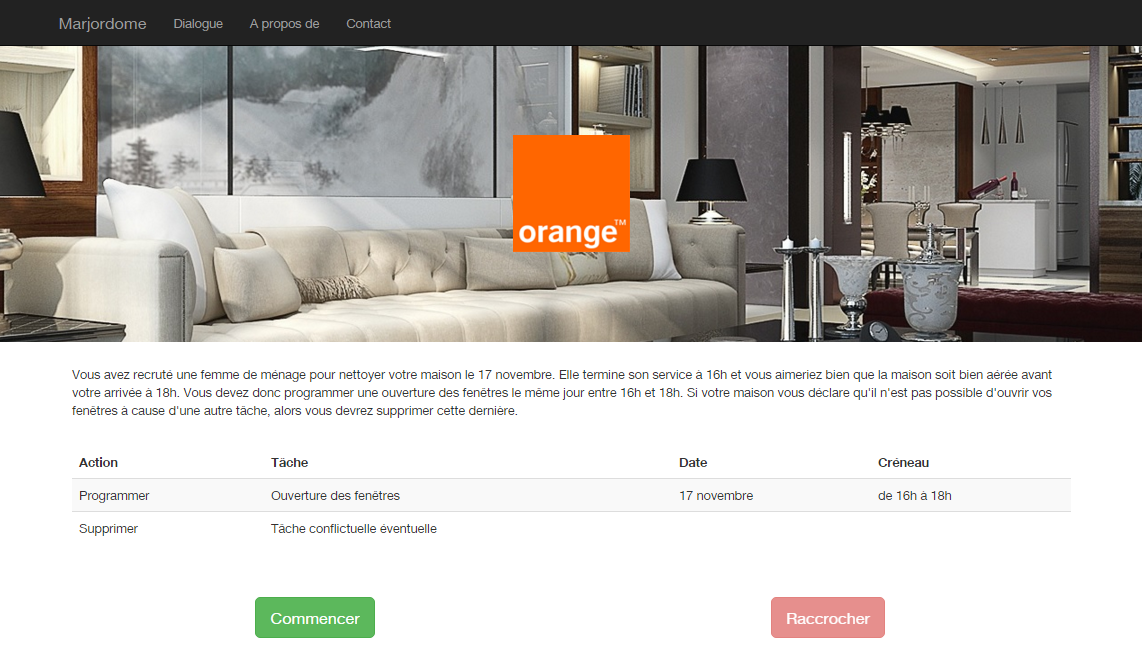
\includegraphics[scale=0.4]{figures/majordome.png}
		\caption{The Majordomo interface}
		\label{fig:majordomo}
	\end{figure*}
	
	\subsection{Key Performance Indicators}
	
		In order to evaluate the three turn-taking strategies, dialogue duration and task completion have been computed (the tasks scheduled by the Majordomo are logged at the end of the dialogue). In addition, the users filled a survey at the end of each dialogue where they provided the following subjective Key Performance Indicators (KPIs):
		
		\begin{itemize}
			\item \textbf{Reactivity:} The users are asked whether they find the system reactive or not. There are 6 possible answers going from 1 (not reactive at all, very slow) to 6 (very reactive).
			\item \textbf{Reactivity impact:} The system's reactivity does not necessarily improve the dialogue quality since it can be perceived as too intrusive. The objective of this metric is to assess the impact associated with the reactivity through 6 possible values going from 1 (very negative, hurts the dialogue quality) to 6 (very positive, significant improvement of the dialogue quality).
			\item \textbf{Realism:} The users are asked whether the system acts like a human operator. There are 6 possible answers going from 1 (no, not at all) to 6 (yes, clearly).
			\item \textbf{Efficiency:} The users are asked to assess the dialogue efficiency by selecting one of the 6 possible answers, going from 1 (very bad) to 6 (very good).
			\item \textbf{Global quality:} The users are asked how they globally appreciated the dialogue on a scale from 1 (Very unpleasant experience) to 6 (Very enjoyable experience).
			\item \textbf{Potential user:} Finally, the users are also asked whether they would use the Majordomo at home (if it was a real commercialised product) on a scale from 1 (clearly not) to 4 (absolutely).
		\end{itemize}


\section{Results and discussion}

	206 dialogues have been collected with the collaboration of 47 volunteer users. 65 dialogues were run using the non-incremental strategy (\textit{None}), 65 using the handcrafted strategy (\textit{Handcrafted}) and 76 using the reinforcement learning one (\textit{RL}). The experiment results are depicted in Table \ref{tab:globalmetrics}.

	\begin{table}[th]
	  \footnotesize
	  \vspace{2mm}
	  \centerline{
	  \begin{tabular}{|c|c|c|c|c|}
	      \hline
	      Category & KPI & \textit{None} & \textit{Handcrafted} & \textit{RL} \\
	      \hline
	      \multirow{2}{*}{Objective} & Duration (sec) & 94.7 & \textbf{89.6} & 90.6 \\
	      & Task completion & 0.60 & 0.63 & \textbf{0.75} \\
	      \hline
	      \multirow{6}{*}{Subjective} & Reactivity & 4.31 & 4.57 & \textbf{4.62} \\
	      & Reactivity quality & \textbf{4.38} & 4.25 & 4.36 \\
	      & Human-likeness & 3.63 & 3.66 & \textbf{3.74} \\
	      & Efficiency & 4.22 & 4.20 & \textbf{4.36} \\
	      & Global quality & 4.06 & 4.18 & \textbf{4.20} \\
	      & Potential use & 2.66 & 2.68 & \textbf{2.82} \\
	      \hline
	  \end{tabular}
	  }
	  \caption{Global dialogue evaluation metrics}
	  \label{tab:globalmetrics}
        \end{table}

        As far as the mean dialogue duration is concerned, the incremental strategies slightly improve the dialogue duration (even though this is not statistically significant). At a first glance, this improvement can be viewed as an obvious result since by construction, incremental strategies are more reactive. Nevertheless, the user can also be interrupted before she has provided all the information that she wanted which complicates the dialogue and makes it last longer like it is the case in the experiment led in \cite{Ghigi2014}. Therefore, this result shows that the Majordomo successfully interrupted the user on average. However, there is no visible change when comparing the \textit{Handcrafted} and the \textit{RL} strategy.

        The task completion ratio, on the other hand, has been significantly\footnote{All the p-values are computed according to the Welch t-test since the number of samples is important enough for the means to be considered as following a normal distribution (and since it is more powerful than non-parametric tests). A binomial proportions test has also been run for task completion, leading to very similar p-values.} improved by the \textit{RL} strategy compared to \textit{None} (by 15\% with $p = 0.030$). Moreover, an important difference has been reported between \textit{RL} and \textit{Handcrafted} (12\%) even though it is not statistically significant at a 0.05 threshold ($p = 0.065$). Finally, \textit{Handcrafted} shows a minor improvement over \textit{None} (3\%) with no statistical significance ($p = 0.36$). The Majordomo task requires a certain level of engagement and focus in order to keep track of all what has been accomplished so far, while keeping the final objective in mind. When interacting with a reactive system that takes the floor in an intelligent way (to correct errors hence fixing desynchronisations, to deliver a response when all the information has been provided...) without overwhelming the user, the latter feels more engaged in the conversation thus accomplishing the task more efficiently, even when a certain cognitive load is involved. Another impact of such strategy as reported in \cite{Ghigi2014} is that when the users realise that they can be interrupted in case of a problem, they tend to provide more concise and focused answers, which reduces the risk of a misunderstanding.

        The subjective metrics are the noisier ones. Therefore, except from the \textit{Reactivity} KPI where \textit{RL} significantly improves it in comparison with \textit{None} ($p = 0.048$), the other p-values are above 0.05. Nevertheless, generally speaking, the metrics are in favour of the \textit{RL} strategy.

	\begin{table}[th]
	  \footnotesize
	  \vspace{2mm}
	  \centerline{
	  \begin{tabular}{|c|c|c|c|}
	      \hline
	      KPI & \textit{None} & \textit{Handcrafted} & \textit{RL} \\
	      \hline
	      Latency (ms) & 1545 $\pm$ 61 & 1303 $\pm$ 78 & \textbf{588 $\pm$ 59} \\
	      FC ratio & No barge-in & 0.31 $\pm$ 0.091 & \textbf{0.068 $\pm$ 0.023} \\
	      \hline
	  \end{tabular}
	  }
	  \caption{Local dialogue evaluation metrics}
	  \label{tab:localmetrics}
	\end{table}

        To complete this study, more local metrics have been investigated: the latency and the false cut-in ratio. The latency is the mean delay involved in each human to machine floor transition\footnote{Estimated as the delay between the moment when the Scheduler delivers the last message and the moment when it received the last ASR output. Computing the real latency requires a Voice Activity Detection (VAD) module in the Client which could slow it down.} (549 transitions for \textit{None}, 542 for \textit{Handcrafted} and 727 for \textit{RL}) whereas the false cut-in ratio refers to the proportion over all the SPEAK decisions (\textit{Handcrafted} : 99, \textit{RL} : 456) of the ones where the system should have waited longer before taking the floor (manually annotated). The results are reported in Table \ref{tab:localmetrics} (all the differences are statistically significant with $p < 0.000001$). The \textit{Handcrafted} strategy reduces the latency by 200ms compared to \textit{None}, however, it interrupts the user too soon one third of the time thus being too aggressive. On the other hand, \textit{RL} reduces the latency by 1 second while maintaining a more reasonable false cut-in ratio. As a consequence, \textit{RL} takes more risk since it chooses to SPEAK more often and when it does, it is better managed.

\section{Discussion}

        In comparison with previous work (see Chapter \ref{ch:stateofart}), this is the first direct application of reinforcement learning to turn-taking management in an incremental dialogue system that is evaluated in real conditions. In many previous studies, an indirect way of testing dialogue strategies is used (controlled dialogue acts \cite{Aist2007}, a posteriori evaluation using recordings of interactions \cite{Meena2013}, a posteriori comparison with human decision corpus \cite{Jonsdottir2008,Dethlefs2012}...). As it is said in \cite{Aist2007}, the objective is \textit{to minimize variance due to extraneous factors such as interspeaker variability, acoustic noise, and so forth and concentrate specifically on the difference between incremental processing and its nonincremental counterpart}. However, the price to pay to reduce variance is a certain bias due to the fact that the experiment is not run in real conditions.

        Some papers use handcrafted strategies \cite{Raux2009,Ghigi2014}, some collect annotated corpora on which they run supervised learning algorithms \cite{Meena2013} and others propose autonomous reinforcement learning based strategies \cite{Selfridge2010,Jonsdottir2008,Dethlefs2012}. However, to our knowledge, live studies only fit in the first two categories and no purely autonomous system using reinforcement learning has been tested with real users and directly evaluated by them, in real dialogue conditions. More generally, previous work related to incremental dialogue processing and turn-taking optimisation can be split into two categories given the metrics that are involved:

        \begin{itemize}
          \item \textbf{Local metrics:} These studies are based on the principle introduced in \cite{Sacks1974} and saying that gaps and overlaps should be minimised in order to achieve smooth turn-taking. As a consequence, local metrics where only floor transitions are considered are used, mainly the latency and the false cut-in ratio \cite{Jonsdottir2008,Raux2012}.
          \item \textbf{Global metrics:} Considering the overall dialogue quality can also be a way of evaluating turn-taking strategies \cite{Selfridge2010,Ghigi2014}. Such an approach has the advantage of not having to make any assumption about what would make the dialogue more appealing for the user. However, the metrics involved are more difficult to measure since they are noisier.
        \end{itemize}

        In this thesis, global metrics were used for training then both global and local metrics were evaluated. Interestingly, it is shown that by optimising global KPIs, local ones turn out to be improved as well. Finally, even though it has been shown that interrupting the user can hurt its opinion on the system in some cases\cite{Hirasawa1999}, the results described above show that when it is done at the right moment, the system is stignificantly more efficient while being judged slightly better from a subjective point of view.


\chapter{A new reinforcement learning approach adapted to incremental dialogue}
\label{ch:theory}

\section{Problem}

\section{Proposed approach}

\section{Toy problem application}

\section{Simulation results}
\chapter*{Conclusion and future work}

	Viewed as a whole, the several contributions made in this thesis constitute a thorough methodology to enhance turn-taking capabilities of spoken dialogue systems. First, turn-taking mechanisms involved in human conversation are analysed which led to the establishment of a new turn-taking phenomena taxonomy. Compared to existing classifications in the literature, new analysis dimensions where the meaning behind the dialogue participants' behaviours, as well as the motivations behind them, are considered. This leads to a more fine-grained taxonomy which is also relevant from the human-machine dialogue point of view. In addition, this constitutes the starting point from which the turn-taking phenomena that are the more likely to improve the dialogue efficiency are chosen.

        An incremental dialogue system can be built from scratch using an incremental version of each component in the dialogue chain. In this thesis, an alternative approach is proposed: a dialogue system is split into a Client and a Service part, then a new module, called the Scheduler, is inserted between the two. This new interface plays the role of a turn-taking manager and makes the set \{Scheduler+Service\} behave as an incremental Service from the Client's point of view. Two advantages are associated with this new approach: first, it makes it possible to transform an existing traditional dialogue system into an incremental one at a low cost and second, the traditional dialogue management part is clearly separated from the turn-taking management one.

        Based on this new architecture, an incremental dialogue simulator has been implemented. It is able to generate dialogues in a personal agenda management domain. A User Simulator, coupled with an ASR Output Simulator that replicates ASR imprefections and instability, sends incremental requests to the Scheduler which decides when to take the floor to provide a response. A first simulation study where several slot-filling strategies along with two turn-taking strategies (incremental and handcrafted incremental) showed that the mixed-initiative one along with incremental processing achieves the best performance in terms of dialogue duration and task completion.

        Since hancrafting turn-taking strategies require the designers to empirically set all the parameters and doing so for each new task, this method is not guaranteed to be optimal while requiring important labour and time resources. On the other hand, data-driven techniques make it possible to build optimal strategies at lower costs. In the field of human-machine dialogue, reinforcement learning has been proven to be particularly useful since no annotation effort is required (unlike supervised techniques) and it is able to learn from delayed rewards (thus making it possible to take the whole dialogue quality as a reward function). In this thesis, a new reinforcement learning turn-taking strategy is proposed and trained using the previous dialogue simulator. In simulation, it has been shown to reduce dialogue duration while improving the task completion ratio when compared to the non-incremental and the handcrafted incremental baselines.

        Finally, the previous strategies have been transposed to a new domain, the Marjordomo, then they have been tested through real users interactions. The handcrafted and the reinforcement learning strategies slightly reduce the dialogue duration, but the latter significantly improves the task completion ratio (by 15\% compared to the non-incremental strategy). Also, compared with the handcrafted strategy, the data-driven one takes more risk by deciding to speak before a user silence (hence significantly reducing the response latency) while maintaining a low false cut-in rate of 6.8\% instead of 31\%.

        To conclude, from a general point of view, this thesis provides new evidence showing the potential of incremental dialogue processing. More particularly, it goes a step further by showing that optimal turn-taking can be learnt automatically during the interactions. Also, the proposed architecture and the generality of the feature used for learning makes it possible to easily transfer this work to any domain and to bootstrap from existing dialogue systems.
        
        During the course of this thesis, two questions were also tackled but due to time constraints, they are still under investigation and there is still work to be done in order to hopefully come up with interesting results. These questions are:

        \begin{itemize}
          \item How to adapt the exploration/exploitation mechanism in reinforcement learning to the case of incremental processing?
          \item How to learn both optimal dialogue management and optimal turn-taking decisions at the same time?
        \end{itemize}

        \paragraph{Exploration/exploitation:} The exploration/exploitation dilemma in reinforcement learning is a research problem in itself. Inspired by the multi-armed bandit literature, the most simple and naive approaches are $\epsilon$-greedy and Boltzmann exploration (Softmax) \cite{Sutton1998} (some other simple approaches also exist in the literature but they are less use and they are based on similar ideas). A new approach (initially proposed to solve the multi-armed bandit problem) called Upper Confidence Bound (UCB) \cite{Auer2002} is also frequently used since it improves the convergence rate. This algorithm has also inspired other algorithms which are more adapted to reinforcement learning like UCRL \cite{Auer2006}. Nevertheless, incremental processing raises a new challenge which is not tackled in existing approaches: in this case, the optimal policy is not balanced when it comes to the number of times each action has to be chosen. The action which consists on doing nothing (called WAIT in this thesis) and wait for further information coming from the ASR should be picked the majority of the time. Therefore, incremental processing involves long episodes where the system should perform one action most of the time and rarely pick an alternative action. As a consequence, during the exploration process using existing methods, the agent rarely performs the right decisions at the right time. Therefore, there is a need to come up with a more adapted and more efficient way to deal with the exploration/exploitation dilemma in this case. In Chapter \ref{ch:rl}, an $\epsilon$-greedy policy with a bias in favour of the WAIT action has been proven to be successful in this case, however, there is no guarantee that this is the optimal way to proceed and more importantly, it is likely that this method performs poorly if the micro-turn duration is increased (imagine a setup with a new micro-turn every millisecond). To investigate this problem, two ideas have been proposed during this thesis:

        \begin{itemize}
          \item \textbf{SMDP-based approach:} Semi-Markov Decision Processes (SMDPs) \cite{Bradtke1994} are different from conventional MDPs in the sense that time is continuous and the time interval between two decisions is not constant (the instants in which the agent is asked to make decisions is defined by a separate process). This is an interesting framework when it comes to incremental dialogue processing and the idea is to cast the Scheduler as an SMDP that is asked to make decisions at specific instants (the rest of the time, it is always picking the WAIT action). Most of the time, when the WAIT action is picked, the state associated with the next micro-turn is very similar to the state associated with the current state. Therefore, the agent will be asked to make decisions only when the state varies in a significant way or in other words, when the state variation given a specific metric reaches a certain threshold. The investigated method tries to learn an optimal value for this threshold in an online fashion.
          \item \textbf{DPS-based approach:} Direct Policy Search (DPS) consists in using classical optimisation methods directly over the policy space unlike conventional reinforcement learning algorithms where a Q-function is computed and then the policy is derived from it. The advantage of such methods is that they naturally embed the mechanism described in the previous point: when two states are similar, a policy is most likely to associate the same action to both of them.
        \end{itemize}

        \paragraph{DM-Scheduler co-learning:} The approach depicted in Chapter \ref{ch:rl} assumes that the dialogue manager (in the Service) has a constant behaviour. However, a very active research thread proposed many methods where this module is constantly improving its decisions mostly using reinforcement learning. Considering that, a natural and legitimate question comes into play: is it possible for both the turn-taking manager and the conventional dialogue manager to simultaneously learn optimal behaviours from interactions. Such a study can benefit from the large existing literature about multi-agent collaborative learning \cite{Claus1998,Panait2005,Vogel2013}.




% ********************************** Back Matter *******************************
% Backmatter should be commented out, if you are using appendices after References
%\backmatter

% ********************************** Bibliography ******************************
\begin{spacing}{0.9}

% To use the conventional natbib style referencing
% Bibliography style previews: http://nodonn.tipido.net/bibstyle.php
% Reference styles: http://sites.stat.psu.edu/~surajit/present/bib.htm

\bibliographystyle{apalike}
%\bibliographystyle{unsrt} % Use for unsorted references  
%\bibliographystyle{plainnat} % use this to have URLs listed in References
\cleardoublepage
\bibliography{biblio}


% If you would like to use BibLaTeX for your references, pass `custombib' as
% an option in the document class. The location of 'reference.bib' should be
% specified in the preamble.tex file in the custombib section.
% Comment out the lines related to natbib above and uncomment the following line.

%\printbibliography[heading=bibintoc, title={References}]


\end{spacing}

% ********************************** Appendices ********************************

\begin{appendices} % Using appendices environment for more functunality

% ******************************* Thesis Appendix A ****************************
\chapter{How to install \LaTeX} 

\section*{Windows OS}

\subsection*{TeXLive package - full version}
\begin{enumerate}
\item	Download the TeXLive ISO (2.2GB) from\\
\href{https://www.tug.org/texlive/}{https://www.tug.org/texlive/}
\item	Download WinCDEmu (if you don't have a virtual drive) from \\
\href{http://wincdemu.sysprogs.org/download/}
{http://wincdemu.sysprogs.org/download/}
\item	To install Windows CD Emulator follow the instructions at\\
\href{http://wincdemu.sysprogs.org/tutorials/install/}
{http://wincdemu.sysprogs.org/tutorials/install/}
\item	Right click the iso and mount it using the WinCDEmu as shown in \\
\href{http://wincdemu.sysprogs.org/tutorials/mount/}{
http://wincdemu.sysprogs.org/tutorials/mount/}
\item	Open your virtual drive and run setup.pl
\end{enumerate}

or

\subsection*{Basic MikTeX - \TeX~ distribution}
\begin{enumerate}
\item	Download Basic-MiK\TeX (32bit or 64bit) from\\
\href{http://miktex.org/download}{http://miktex.org/download}
\item	Run the installer 
\item	To add a new package go to Start >> All Programs >> MikTex >> Maintenance (Admin) and choose Package Manager
\item	Select or search for packages to install
\end{enumerate}

\subsection*{TexStudio - \TeX~ editor}
\begin{enumerate}
\item	Download TexStudio from\\
\href{http://texstudio.sourceforge.net/\#downloads}
{http://texstudio.sourceforge.net/\#downloads} 
\item	Run the installer
\end{enumerate}

\section*{Mac OS X}
\subsection*{MacTeX - \TeX~ distribution}
\begin{enumerate}
\item	Download the file from\\
\href{https://www.tug.org/mactex/}{https://www.tug.org/mactex/}
\item	Extract and double click to run the installer. It does the entire configuration, sit back and relax.
\end{enumerate}

\subsection*{TexStudio - \TeX~ editor}
\begin{enumerate}
\item	Download TexStudio from\\
\href{http://texstudio.sourceforge.net/\#downloads}
{http://texstudio.sourceforge.net/\#downloads} 
\item	Extract and Start
\end{enumerate}


\section*{Unix/Linux}
\subsection*{TeXLive - \TeX~ distribution}
\subsubsection*{Getting the distribution:}
\begin{enumerate}
\item	TexLive can be downloaded from\\
\href{http://www.tug.org/texlive/acquire-netinstall.html}
{http://www.tug.org/texlive/acquire-netinstall.html}.
\item	TexLive is provided by most operating system you can use (rpm,apt-get or yum) to get TexLive distributions
\end{enumerate}

\subsubsection*{Installation}
\begin{enumerate}
\item	Mount the ISO file in the mnt directory
\begin{verbatim}
mount -t iso9660 -o ro,loop,noauto /your/texlive####.iso /mnt
\end{verbatim}

\item	Install wget on your OS (use rpm, apt-get or yum install)
\item	Run the installer script install-tl.
\begin{verbatim}
	cd /your/download/directory
	./install-tl
\end{verbatim}
\item	Enter command `i' for installation

\item	Post-Installation configuration:\\
\href{http://www.tug.org/texlive/doc/texlive-en/texlive-en.html\#x1-320003.4.1}
{http://www.tug.org/texlive/doc/texlive-en/texlive-en.html\#x1-320003.4.1} 
\item	Set the path for the directory of TexLive binaries in your .bashrc file
\end{enumerate}

\subsubsection*{For 32bit OS}
For Bourne-compatible shells such as bash, and using Intel x86 GNU/Linux and a default directory setup as an example, the file to edit might be \begin{verbatim}
edit $~/.bashrc file and add following lines
PATH=/usr/local/texlive/2011/bin/i386-linux:$PATH; 
export PATH 
MANPATH=/usr/local/texlive/2011/texmf/doc/man:$MANPATH;
export MANPATH 
INFOPATH=/usr/local/texlive/2011/texmf/doc/info:$INFOPATH;
export INFOPATH
\end{verbatim}
\subsubsection*{For 64bit OS}
\begin{verbatim}
edit $~/.bashrc file and add following lines
PATH=/usr/local/texlive/2011/bin/x86_64-linux:$PATH;
export PATH 
MANPATH=/usr/local/texlive/2011/texmf/doc/man:$MANPATH;
export MANPATH 
INFOPATH=/usr/local/texlive/2011/texmf/doc/info:$INFOPATH;
export INFOPATH

\end{verbatim}



%\subsection{Installing directly using Linux packages} 
\subsubsection*{Fedora/RedHat/CentOS:}
\begin{verbatim} 
sudo yum install texlive 
sudo yum install psutils 
\end{verbatim}


\subsubsection*{SUSE:}
\begin{verbatim}
sudo zypper install texlive
\end{verbatim}


\subsubsection*{Debian/Ubuntu:}
\begin{verbatim} 
sudo apt-get install texlive texlive-latex-extra 
sudo apt-get install psutils
\end{verbatim}

% ******************************* Thesis Appendix B ********************************

\chapter{Installing the CUED class file}

\LaTeX.cls files can be accessed system-wide when they are placed in the
<texmf>/tex/latex directory, where <texmf> is the root directory of the user’s \TeX installation. On systems that have a local texmf tree (<texmflocal>), which
may be named ``texmf-local'' or ``localtexmf'', it may be advisable to install packages in <texmflocal>, rather than <texmf> as the contents of the former, unlike that of the latter, are preserved after the \LaTeX system is reinstalled and/or upgraded.

It is recommended that the user create a subdirectory <texmf>/tex/latex/CUED for all CUED related \LaTeX class and package files. On some \LaTeX systems, the directory look-up tables will need to be refreshed after making additions or deletions to the system files. For \TeX Live systems this is accomplished via executing ``texhash'' as root. MIK\TeX users can run ``initexmf -u'' to accomplish the same thing.

Users not willing or able to install the files system-wide can install them in their personal directories, but will then have to provide the path (full or relative) in addition to the filename when referring to them in \LaTeX.

\end{appendices}

% *************************************** Index ********************************
\printthesisindex % If index is present

\end{document}
